\documentclass[12pt,french,oneside]{report}
%%%%%%%%%%%%%%%%%%%%%%%%%%%%%%%%%%%%%%%%%%%%%%%%%%%%%%%%%%%%%%%%%%%%%%%%%%%%%%%
%___________________________
%===    Configurations 12.09.2013
%------------------------------------------------------
%packages permettant d'augmenter le nombre de registres de dimension et donc d'éviter les erreurs de compilation dûs aux packages tikz, pstricks and compagnie
\usepackage{etex}
%___________________________
%===    Pour le français
%------------------------------------------------------
\usepackage[utf8x]{inputenc}
\usepackage[T1]{fontenc}
\usepackage[english,french]{babel}
\FrenchFootnotes
\usepackage{tipa}%alphabet phonétique internationnal
%___________________________
%===    Polices d'écriture
%------------------------------------------------------
%\usepackage{mathpazo}
\usepackage{frcursive} % Pour l'écriture cursive
\usepackage[upright]{fourier}% l'option permet d'avoir les majuscules droites dans les formules mathématiques
\usepackage[scaled=0.875]{helvet}

%___________________________
%===    Les couleurs
%------------------------------------------------------
\usepackage[dvipsnames,table]{xcolor}
%
\newcommand{\rouge}[1]{{\color{red} #1}}
\definecolor{midblue}{rgb}{0.145,0.490,0.882}
\newcommand\MaCouleur{midblue}

%___________________________
%===   Entête, pied de page
%------------------------------------------------------

\usepackage{lscape} %permet le format paysage du document
\usepackage{xspace} % création automatique d'espaces dans les commandes
\setlength{\parindent}{0pt}

\usepackage{fancyhdr}
%
\renewcommand{\headrulewidth}{0pt}% pas de trait en entête
\newcommand\RegleEntete[1][0.4pt]{\renewcommand{\headrulewidth}{#1}}%commande pour ajouter un trait horizontal en entête

\newcommand{\entete}[3]{\lhead{#1} \chead{#2} \rhead{#3}}
\newcommand{\pieddepage}[3]{\lfoot{#1} \cfoot{#2} \rfoot{#3}}

\renewcommand{\chaptermark}[1]{\markboth{#1}{}} % enregistre le titre courant du chapitre 
%en-tete droite page [paire] et {impaire}
\rhead[]{\textbf{\leftmark.}}
%en-tete gauche page [paire] et {impaire}
\lhead[\textbf{\chaptername~\thechapter.}]{}


\usepackage{enumerate} %permet la modif de la numérotation et de poursuivre une numérotation en cours avec \begin{enumerate}[resume]
\usepackage{enumitem}
\frenchbsetup{StandardLists=true}%frenchb ne s'occupera pas des listes
\setenumerate[1]{font=\bfseries,label=\arabic*.} % numérotation 1. 2. ...
%\setenumerate[2]{font=\itshape,label=(\alph*)} % sous-numérotation (a) (b) ...
\setenumerate[2]{font=\bfseries,label=\alph*)} % sous-numérotation a) b) ...

\usepackage{lastpage} % permet d'afficher le nombre total de pages après DEUX compilations.

%___________________________
%===    Raccourcis classe
%------------------------------------------------------
\newcommand\seconde{2\up{nde}\xspace}
\newcommand\premiere{1\up{ère}\xspace}
\newcommand\terminale{T\up{le}\xspace}
\newcommand\stmg{\bsc{Stmg}}
\newcommand\sti{\bsc{Sti2d}}
\newcommand\bat{BAT 1\xspace}
\newcommand\BAT{BAT 2\xspace}
\newcommand\tesspe{TES Spécialité\xspace}


%___________________________
%===    Réglages et Commandes Maths
%------------------------------------------------------
%les commandes suivantes évitent le message "too many math alphabets"...
\newcommand\hmmax{0}
\newcommand\bmmax{0}

%redéfinition de fractions, limites, sommes, intégrales, coefficients binomiaux en displaystyle, limites de suites
\usepackage{amssymb,mathtools}
\let\binomOld\binom
\renewcommand{\binom}{\displaystyle\binomOld}
\let\limOld\lim
\renewcommand{\lim}{\displaystyle\limOld}
\newcommand{\limn}{\lim_{n\to +\infty}} %limite lorsque n tend vers + infini
\newcommand{\limm}{\lim_{x\to -\infty}} %limite lorsque x tend vers - infini
\newcommand{\limp}{\lim_{x\to +\infty}} %limite lorsque x tend vers + infini
\newcommand{\limz}{\lim_{x\to 0}} %limite lorsque x tend vers 0
\newcommand{\limzm}{\lim_{\substack{x \to 0\\ x < 0}}} %limite lorsque x tend vers 0-
\newcommand{\limzp}{\lim_{\substack{x \to 0\\ x > 0}}} %limite lorsque x tend vers 0+
\let\sumOld\sum
\renewcommand{\sum}{\displaystyle\sumOld}
\let\intOld\int
\renewcommand{\int}{\displaystyle\intOld}

%\usepackage{yhmath}%permet les arcs de cercles
%\usepackage[euler-digits]{eulervm} %-> police maths
%
\usepackage{stmaryrd}%\llbracket et \rrbracket % crochets doubles pour intervalles d'entier
%symbole parallèle avec \sslash

\newcommand{\crochets}[2]{\ensuremath{\llbracket #1 ; #2 \rrbracket}}

\newcommand{\intervalleff}[2]{\left[#1\,;#2\right]}
\newcommand{\intervallefo}[2]{\left[#1\,;#2\right[}
\newcommand{\intervalleof}[2]{\left]#1\,;#2\right]}
\newcommand{\intervalleoo}[2]{\left]#1\,;#2\right[}



\usepackage{bm} % pour l'écriture en gras des formules mathématiques avec \bm

\usepackage{cancel} % pour les simplifications de fractions
\renewcommand\CancelColor{\color{red}}
%\usepackage{siunitx} % écriture de nombres et d'unités
%\sisetup{output-decimal-marker={,},detect-all}
\usepackage[autolanguage,np]{numprint}
%permet les espacement pour les nombres décimaux avec \np{3,12456} en environnement maths ou pas
\DecimalMathComma %supprime l'espace après la virgule dans un nombre

%
\usepackage{dsfont} %écriture des ensemble N, R, C ...
\newcommand{\C}{\mathds C}
\newcommand{\R}{\mathds R}
\newcommand{\Q}{\mathds Q}
\newcommand{\D}{\mathds D}
\newcommand{\Z}{\mathds Z}
\newcommand{\N}{\mathds N}
\newcommand\Ind{\mathds 1} %= fonction indicatrice
\newcommand\p{\mathds P} %= probabilité
\newcommand\E{\mathds E} % Espérance
\newcommand\V{\mathds V} % Variance
\newcommand{\e}{\text{e}}
\newcommand{\dd}{\,\text{d}}

%Nombres complexes
\let\Reold\Re
\renewcommand{\Re}{~\text{Re}~}
\let\Imold\Im
\renewcommand{\Im}{~\text{Im}~}
\newcommand{\ii}{\,\text{i}}
% Exponentielle complexe
\newcommand{\ei}[2]{\,\e^{\dfrac{#1\ii\pi}{#2}}}


%
\usepackage{mathrsfs}   % Police de maths jolie caligraphie
\newcommand{\calig}[1]{\ensuremath{\mathscr{#1}}}
\newcommand\mtc[1]{\ensuremath{\mathcal{#1}}}


%Gestion des espaces
%
\newcommand{\pv}{\ensuremath{\: ; \,}}
\newlength{\EspacePV}
\setlength{\EspacePV}{1em plus 0.5em minus 0.5em}
\newcommand{\qq}{\hspace{\EspacePV} ; \hspace{\EspacePV}}
\newcommand{\qetq}{\hspace{\EspacePV} \text{et} \hspace{\EspacePV}}
\newcommand{\qouq}{\hspace{\EspacePV} \text{ou} \hspace{\EspacePV}}
\newcommand{\qLq}{\hspace{\EspacePV} \Leftarrow \hspace{\EspacePV}}
\newcommand{\qRq}{\hspace{\EspacePV} \Rightarrow \hspace{\EspacePV}}
\newcommand{\qLRq}{\hspace{\EspacePV} \Leftrightarrow \hspace{\EspacePV}}

%simplification notation norme \norme{}
\newcommand{\norme}[1]{\left\Vert #1\right\Vert}


%simplification de la notation de vecteur \vect{}
\newcommand{\vect}[1]{\mathchoice%
{\overrightarrow{\displaystyle\mathstrut#1\,\,}}%
{\overrightarrow{\textstyle\mathstrut#1\,\,}}%
{\overrightarrow{\scriptstyle\mathstrut#1\,\,}}%
{\overrightarrow{\scriptscriptstyle\mathstrut#1\,\,}}}



%Repères
\def\Oij{$\left(\text{O}\pv\vect{\imath},~\vect{\jmath}\right)$\xspace}
\def\Oijk{$\left(\text{O}\pv\vect{\imath},~ \vect{\jmath},~ \vect{k}\right)$\xspace}
\def\Ouv{$\left(\text{O}\pv\vect{u},~\vect{v}\right)$\xspace}
\def\OIJ{$\left(O\pv I\:,\,J\right)$\xspace}

\newcommand\abs[1]{\ensuremath{\left\vert #1 \right\vert}}%valeur absolue
\newcommand\Arc[1]{\ensuremath{\wideparen{#1}}}%arc de cercle


%symbole pour variable aléatoire qui suit une loi
\newcommand{\suit}{\hookrightarrow}

%___________________________
%===    Pour les tableaux
%------------------------------------------------------
\usepackage{array}
\usepackage{longtable}
\usepackage{tabularx,tabulary}
\usepackage{multirow}
\usepackage{multicol}
%exemple
%\begin{multicols}{3}[Titre sur une seule colonne.]
%   3~colonnes équilibrées, 3~colonnes équilibrées, 3~colonnes équilibrées, 3~colonnes équilibrées
%\end{multicols}
%\begin{multicols}{2}[\section{Titre numéroté.}]
%   blabla sur deux colonnes, c'est plus sérieux. C'est le style qui est généralement utilisé pour écrire des articles.
%saut de colonne forcé :
%\columnbreak
%djhskjdhjsq
%sdkksqjhd
%\end{multicols}
%Pour ajouter un titre numéroté qui apparaisse sur toute la largeur de la page, il faut utiliser l'option [\section{Titre.}] juste après \begin{multicols}{nb-col}.
%Remarques :
%Pour qu'une ligne de séparation apparaisse entre les colonnes, il faut utiliser : \setlength{\columnseprule}{1pt}.

%Pour redéfinir la largeur de l'espace inter-colonnes, il faut utiliser \setlength{\columnsep}{30pt}.

%Pour remonter le texte, dans chaque colonne vers le haut : \raggedcolumns qui se tape :\begin{multicols}{2}\raggedcolumns...\columnbreak...\columnbreak\end{multicols}

%Pour supprimer les traits verticaux : \setlength{\columnseprule}{0pt} avant \begin{multicols}{3}...\end{multicols}
\setlength\columnseprule{0.4pt}
\renewcommand{\arraystretch}{1.5}%augmente la hauteur des lignes des tableaux
%colonnes centrées verticalement et horizontalement permettant d'écrire des paragraphes de largeur fixée du type M{3cm}
\newcolumntype{M}[1]{>{\centering\arraybackslash}m{#1}}%cellule centrée horizontalement et verticalement
\newcolumntype{R}[1]{>{\raggedleft\arraybackslash}m{#1}}%cellule alignée à droite et centrée verticalement
%\arraybackslash permet de continuer à utiliser \\ pour le changement de ligne

\usepackage{arydshln}% permet des filets horizontaux ou verticaux en pointillés avec
%pour les filets horizontaux \hdashline ou \cdashline qui s'utilisent comme \hline ou \cline
% pour les filets verticaux les deux points :


%___________________________
%===    Divers packages
%------------------------------------------------------
\usepackage{bclogo}
\usepackage{textcomp}
\usepackage{eurosym}%avec \EUR{3,12}
\usepackage{soul} % Pour souligner : \ul
\usepackage{ulem} % Pour souligner double : \uuline
                      % Pour souligner ondulé : \uwave
                      % Pour barrer horizontal : \sout
                      % Pour barrer diagonal : \xout
\usepackage{tikz,tkz-base,tkz-fct,tkz-euclide,tkz-tab,tkz-graph,tikz-3dplot}
\usetkzobj{all}
\usetikzlibrary{calc,shapes,arrows,plotmarks,lindenmayersystems,decorations,decorations.markings,decorations.pathmorphing,
decorations.pathreplacing,patterns,positioning,decorations.text}
\usetikzlibrary{shadows,trees}
\usepackage{pstricks,pst-plot,pst-text,pstricks-add,pst-eucl,pst-all}

\usepackage{pgfplots}


%INTERLIGNES
\usepackage{setspace}
%s'utilise avec \begin{spacing}{''facteur''}
%   […]
%\end{spacing}

%Pointillés sur toute la ligne
\usepackage{multido}
\newcommand{\Pointilles}[1][1]{%
\multido{}{#1}{\makebox[\linewidth]{\dotfill}\\[1.5\parskip]
}}
%commandes : \Pointilles ou \Pointilles[4] pour 4 lignes


%textes à trous
\newlength\lgtrou
\newcommand*\trou[1]{%
\settowidth\lgtrou{#1}%
\makebox[2\lgtrou]{\dotfill}
\setlength\baselineskip{1.2\baselineskip}}
%Commande à utiliser : \trou{texte qui sera remplacé par des pointillés}

%divers cadres
\usepackage{fancybox} % par exemple \ovalbox{}

%caractères spéciaux avec la commande \ding{230} par exemple
\usepackage{pifont}

%___________________________
%===    Quelques raccourcis perso
%------------------------------------------------------
\newcommand\pfr[1]{\psframebox[linecolor=red]{#1}}
\newcommand\coef[1][]{c{\oe}fficient#1\xspace}

%checked box
\newcommand{\checkbox}{
\makebox[0pt][l]{$\square$}\raisebox{.15ex}{\hspace{0.1em}$\checkmark$}
}

%QRcode, codebarre
\usepackage{pst-barcode}
%\begin{pspicture}(2,2)
%	\psbarcode{http://www.latex-howto.be}{eclevel=M}{qrcode}
%\end{pspicture}


%Texte en filigrane
\usepackage{watermark}
%On utilise ensuite les commandes \watermark, \leftwatermark, \rightwatermark ou \thiswatermark qui permettent de définir un filigrane sur toutes les pages, les pages paires, les pages impaires ou juste une page
%Exemple : \thiswatermark {
%\begin{minipage}{0.95\linewidth}
%\vspace{25cm}
%\begin{center}
%\rotatebox{55}{\scalebox{8}{\color[gray]{0.7}\LaTeX}}
%\end{center}
%\end{minipage}
%}

%QCM
\usepackage{alterqcm}					%%Permet de créer des QCM
%\begin{alterqcm}
%\AQquestion{Question}{{Proposition 1},{Proposition 2},{Proposition 3}}
%\end{alterqcm}

%\dingsquare %carré avant V ou F
%\dingchecksquare %carré validé devant V ou F


%Rond entourant une lettre avec pour arguments la couleur de fond, puis la lettre
\newcommand\rond[2][red!20]{\tikz[baseline]{\node[fill=#1,anchor=base,circle]{\bf #2};}}


%Ecrire card en écriture normale :
\newcommand{\card}{\text{card}\xspace}


%___________________________
%===    ALGORITHMES
%------------------------------------------------------

%ALGORITHME avec Algobox
\usepackage{ucs}
\usepackage{framed}
\definecolor{fond}{gray}{0.95}
\newenvironment{cadrecode}{%
  \def\FrameCommand{{\color[HTML]{888888}\vrule width 3pt}\colorbox{fond}}%
  \MakeFramed {\advance\hsize-\width \FrameRestore}}%
{\endMakeFramed}
\usepackage{alltt}

% Mise en forme des algorithmes
\usepackage[french,boxed,titlenumbered,lined,longend]{algorithm2e}
  \SetKwIF {Si}{SinonSi}{Sinon}{si}{alors}{sinon\_si}{alors}{fin~si}
 \SetKwFor{Tq}{tant\_que~}{~faire~}{fin~tant\_que}
 \SetKwFor{PourCh}{pour\_chaque }{ faire }{fin pour\_chaque}
 \SetKwInput{Sortie}{Sortie}
  \SetKwInput{Entree}{Entrée}
\newcommand{\Algocmd}[1]{\textsf{\textsc{\textbf{#1}}}}\SetKwSty{Algocmd}
  \newcommand{\AlgCommentaire}[1]{\textsl{\small  #1}}
  
%Autres packages de Stéphane Pasquet
\usepackage{pas-algo}
\usepackage{tcolorbox}

%exemple :
%\begin{center}
%\textbf{À compiler en pdfLaTeX}
%\end{center}
%
%
%\begin{center}
%\begin{algo}[somsuitar]{Calcul d'une somme}
%\begin{algovar}
%r est un nombre réel \\
%u est un nombre réel \\
%n est un entier naturel \\
%i est un entier naturel \\
%S est un nombre réel
%\end{algovar}
%\begin{algoentries}
%r est un nombre réel \\
%u est un nombre réel \\
%n est un entier naturel \\
%i est un entier naturel \\
%S est un nombre réel
%\end{algoentries}
%\begin{algoinit}
%Affecter à S la valeur u\\
%Entrer la valeur de r ( raison de la suite arithmétique )\\
%Entrer la valeur de u ( premier terme de la somme )\\
%Entrer la valeur de n ( nombre de termes dans la somme )
%\end{algoinit}
%\begin{algobody}
%\begin{algofor}{i}{1}{n-1}
%Affecter à S la valeur S+(u+i*r)
%\end{algofor}
%\end{algobody}
%\begin{algoend}
%Afficher S
%\end{algoend}
%\end{algo}
%\end{center}
%
%
%
%L'algorithme \ref{algo:somsuitar} permet de calculer la somme 
%$u_p+u_{p +1}+ u_{p +2}+\cdots +u_{p+n -1}$ , où $(u)$ est une suite
%arithmétique de raison $r$. La valeur de $u$ saisie lors de l'initialisation est la valeur de $u_p$.




%___________________________
%===    MISE EN FORME EXERCICES
%------------------------------------------------------
%\usepackage{marvosym}
\usepackage{slashbox}

\newcounter{exo}
\newenvironment{exo}{%
  \refstepcounter{exo}\Writinghand\ \textbf{Exercice \theexo.}\par
  \medskip}%
{\[*\]}


%___________________________
%===    HYPERLIENS
%------------------------------------------------------
\usepackage[colorlinks=true,linkcolor=black,filecolor=blue,urlcolor=blue,bookmarksnumbered]{hyperref} 


%___________________________
%===    SOMMAIRE DANS LES CHAPITRES
%------------------------------------------------------

\usepackage{minitoc}

%___________________________
%===    TABLEUR
%------------------------------------------------------
\usepackage{pas-tableur}%package de Stéphane Pasquet
\usepackage{xstring}
\usepackage{xkeyval}


%___________________________
%===    touches calculatrices
%------------------------------------------------------

\newcommand{\touche}[1]{\begin{pspicture}(0,0)(0.9,0.4)\psframe[framearc=0.5,shadow=true,shadowcolor=gray!50](0,0)(0.8,0.45)\rput[cc](0.4,
0.225){#1}\end{pspicture}} %touche calculatrice
\newcommand{\gtouche}[1]{\begin{pspicture}(0,0)(1.8,0.4)\psframe[framearc=0.5,shadow=true,shadowcolor=gray!50](0,0)(1.6,0.45)\rput[cc](0.8,
0.225){#1}\end{pspicture}} %grande touche calculatrice
\newcommand{\ggtouche}[1]{\begin{pspicture}(0,0)(2.4,0.4)\psframe[framearc=0.5,shadow=true,shadowcolor=gray!50](0,0)(2.4,0.45)\rput[cc](1.2,
0.225){#1}\end{pspicture}} %grande touche calculatrice

\usepackage{tipfr}
%___________________________
%===   Redéfinition des marges par défaut
%------------------------------------------------------
%\usepackage[textwidth=18.6cm]{geometry}%à mettre dans le preambule perso
%\pagestyle{fancy}%à mettre dans le preambule perso


\setlength\paperheight{297mm}
\setlength\paperwidth{210mm}
\setlength{\evensidemargin}{0cm}% Marge gauche sur pages paires
\setlength{\oddsidemargin}%{0cm}%
{-0.5cm}% Marge gauche sur pages impaires
\setlength{\topmargin}{-2cm}% Marge en haut
\setlength{\headsep}{0.5cm}% Entre le haut de page et le texte
\setlength{\headheight}{0.7cm}% Haut de page
\setlength{\textheight}{25.2cm}% Hauteur de la zone de texte
\setlength{\textwidth}{17cm}% Largeur de la zone de texte


% Environnement enumerate
\renewcommand{\theenumi}{\bf\textsf{\arabic{enumi}}}
\renewcommand{\labelenumi}{\bf\textsf{\theenumi.}}
\renewcommand{\theenumii}{\bf\textsf{\alph{enumii}}}
\renewcommand{\labelenumii}{\bf\textsf{\theenumii.}}
\renewcommand{\theenumiii}{\bf\textsf{\roman{enumiii}}}
\renewcommand{\labelenumiii}{\bf\textsf{\theenumiii.}}


\usetikzlibrary{shadows,trees}


%definition des couleurs
\definecolor{fondpaille}{cmyk}{0,0,0.1,0}%\pagecolor{fondpaille}
\definecolor{gris}{rgb}{0.7,0.7,0.7}
\definecolor{rouge}{rgb}{1,0,0}
\definecolor{bleu}{rgb}{0,0,1}
\definecolor{vert}{rgb}{0,1,0}
\definecolor{deficolor}{HTML}{2D9AFF}
\definecolor{backdeficolor}{HTML}{EDEDED}%{036DD0}%dégradé bleu{666666}%dégradé gris
\definecolor{theocolor}{HTML}{C10CC7}%{HTML}{036DD0}%F4404D%rouge
\definecolor{backtheocolor}{HTML}{D3D3D3}
\definecolor{methcolor}{HTML}{008800}%12BB05}
\definecolor{backmethcolor}{HTML}{FFFACD}
\definecolor{backilluscolor}{HTML}{EDEDED}
\definecolor{sectioncolor}{HTML}{C10CC7}%{B2B2B2}%vert : {HTML}{008800}%{HTML}{2D9AFF}
\definecolor{subsectioncolor}{HTML}{C10CC7}%{B2B2B2}%vert : {HTML}{008800}%{rgb}{0.5,0,0}
\definecolor{subsubsectioncolor}{HTML}{C10CC7}
\definecolor{engcolor}{HTML}{D4D7FE}
\definecolor{exocolor}{rgb}{0,0.6,0}
\definecolor{exosoltitlecolor}{rgb}{0,0.6,0}
\definecolor{titlecolor}{rgb}{1,1,1}

%commande pour enlever les couleurs avant impression
\newcommand{\nocolor}
{\pagecolor{white}
\definecolor{gris}{rgb}{0.7,0.7,0.7}
\definecolor{rouge}{rgb}{0,0,0}
\definecolor{bleu}{rgb}{0,0,0}
\definecolor{vert}{rgb}{0,0,0}
\definecolor{deficolor}{HTML}{B2B2B2}
\definecolor{backdeficolor}{HTML}{EEEEEE}%{036DD0}%dégradé bleu{666666}%dégradé gris
\definecolor{theocolor}{HTML}{B2B2B2}
\definecolor{backtheocolor}{HTML}{EEEEEE}
\definecolor{methcolor}{HTML}{B2B2B2}
\definecolor{backmethcolor}{HTML}{EEEEEE}
\definecolor{backilluscolor}{HTML}{EEEEEE}
\definecolor{sectioncolor}{HTML}{B2B2B2}
\definecolor{subsectioncolor}{HTML}{B2B2B2}
\definecolor{subsubsectioncolor}{HTML}{B2B2B2}
\definecolor{engcolor}{HTML}{EEEEEE}
\definecolor{exocolor}{HTML}{3B3838}
\definecolor{exosoltitlecolor}{rgb}{0,0,0}
\definecolor{titlecolor}{rgb}{0,0,0}
}



%%%%%%%%%%%%%%%%%%%%%%%%%%%%%%%%%%%%%%%%%%%%%%%%%%%%%%%%%%%%%%%%%%%%%%%%%%%%%%%
%Encadrés pour Propriétés, Théorème, Définitions, exemples, exercices

\usepackage{environ}%pour pouvoir utiliser la commande \NewEnviron

%___________________________
%===    Cadre arrondi coloré
%------------------------------------------------------
%
\NewEnviron{CadreColor}{
\medskip
\begin{tikzpicture}[node distance=0 cm]
\node[draw,drop shadow,color=theocolor,very thick,fill=backtheocolor,rounded corners=5pt,anchor=north west] at(0,-0.02)
{\black\parbox{\linewidth-12pt}{\BODY}};
\end{tikzpicture}
%\medskip
}


%___________________________
%===    Cadre arrondi blanc
%------------------------------------------------------
%
\NewEnviron{Cadre}{
\medskip
\begin{tikzpicture}[node distance=0 cm]
\node[draw,very thick,rounded corners=5pt,anchor=north west] at(0,-0.02)
{\black\parbox{\linewidth-12pt}{\BODY}};
\end{tikzpicture}
%\medskip
}




%___________________________
%===    Redéfinition de la commande \chapter{•}
%------------------------------------------------------
%
\makeatletter

\renewcommand{\@makechapterhead}[1]{
{\color{blue}
        \begin{flushright}
            \fontfamily{pzc}
            \bfseries\fontsize{40}{20}\selectfont{
            #1}
            
        \end{flushright}
        \vspace{24pt}
            %\rule{\linewidth}{1pt}
            }
\setlength\parindent{0mm}
\renewcommand \footrulewidth{0.2pt}%
\renewcommand \headrulewidth{0pt}%
\pagestyle{fancy}
\fancyhf{}
\pieddepage{\leftmark}{}{\thepage / \pageref{LastPage}}
}

%Chapitre avec effet miroir en dessous
%{\begin{tikzpicture}[remember picture, overlay,shift={(current page.north east)}]
%        \node at (0.1,0.1) [below left,draw=\MaCouleur, very thick,rounded corners, inner sep=10pt, inner ysep=10pt,fill=gray!20,text width=3cm, align=center]%
%            {\small\color{\MaCouleur}
%            \bfseries \bsc{\chaptername \thechapter}};
%    \end{tikzpicture}\vspace*{-2cm}
%
%    \begin{center}
%        \begin{tikzpicture}[color={\MaCouleur}]
%            \draw (0,0) -- (0.8\linewidth,0)
%                node[midway,above] {\fontfamily{pzc}\selectfont\scalefont{3}#1}
%                node[midway,above,yscale=-1, opacity=0.5] {\fontfamily{pzc}\selectfont\scalefont{3}#1};
%        \end{tikzpicture}
%    \end{center}
%}

%Chapitre encadré en couleur
%{
%\begin{tikzpicture}
%\node[fill=theocolor,rectangle,rounded corners=5pt]{%
%\begin{minipage}{\linewidth}
%\begin{center}
%\vspace*{9pt}
%\textcolor{titlecolor}{\Large \textsc{\textbf{Chapitre \thechapter \ : \ #1}}}
%\vspace*{9pt}
%\end{center}
%\end{minipage}
%};\end{tikzpicture}
%}

\makeatother


%___________________________
%===    Commandes perso
%------------------------------------------------------
%
%\Leftrightarrow
\newcommand{\Lr}{\Leftrightarrow}

%Ancienne commande chapitre
\newcommand{\chapitre}[1]{
\begin{tikzpicture}
\node[fill=sectioncolor,rectangle,rounded corners=5pt]{%
\begin{minipage}{\linewidth}
\begin{center}
\vspace*{9pt}
\textcolor{titlecolor}{\Large \textsc{\textbf{#1}}}
\vspace*{9pt}
\end{center}
\end{minipage}
};
\end{tikzpicture}
\bigskip
}


\pagecolor{white}%couleur du fond de page

\renewcommand{\Pointilles}{%
\makebox[\linewidth]{\dotfill}
}


%QRcode généré par le package qrcode
\usepackage{qrcode}


%Pour pouvoir utiliser l'environnement verbatim
\usepackage{verbatim}

%Panneau danger (nécessite le package pstricks)
\def\danger{\begingroup
\psset{unit=1ex}%
\begin{pspicture}(0,0)(3,3)
 
\pspolygon[linearc=0.2,linewidth=0.12,linecolor=red](0,0)(1.5,2.6)(3,0)
 
\psellipse*(1.5,1.33)(0.14,0.75)\pscircle*(1.5,0.3){0.15}\end{pspicture}
%
\endgroup}%

\newcommand{\cad}{c'est-à-dire }



%%%%%%%%%%%%%%%%%%%%%%%%%%%%%%%%%%%%%%%%%%%%%%%%%%%%%%%%%%%%%%%%%%%%%%%%%%%%%%%
%--------------------- PRESENTATION SECTIONS
\usepackage{titlesec}
\setcounter{secnumdepth}{3}
\makeatletter

% couleurs section
\definecolor{section@title@color}{cmyk}{1,0.2,0.3,0.1}
\definecolor{subsection@title@color}{cmyk}{0,0.6,0.9,0}
\definecolor{subsubsection@title@color}{cmyk}{1,0.2,0.3,0.1}
\definecolor{shadow@color}{cmyk}{.07,0,0,0.49}

% fontes section
\def\sectiontitle@font{\fontfamily{ppl}\fontseries{bx}\selectfont}
%\def\subsectiontitle@font{\fontfamily{ppl}\fontseries{bx}\selectfont}
%\def\subsubsectiontitle@font{\fontfamily{ppl}\fontseries{bx}\selectfont}

% Décalages numéro de sections / titres des sections
\newlength\decalnumsec
\newlength\decalnumsubsec
\newlength\decalnumsubsubsec
\setlength{\decalnumsec}{-0.5em}
\setlength{\decalnumsubsec}{-0.5em}
\setlength{\decalnumsubsubsec}{-0.5em}
\newlength\decalxtitlesec
\newlength\decalxtitlesubsec
\newlength\decalxtitlesubsubsec
\setlength{\decalxtitlesec}{-2.45em}
\setlength{\decalxtitlesubsec}{-1em}
\setlength{\decalxtitlesubsubsec}{0.45em}

% Espace entre le numéro de section et le titre
\newlength\spacetitlesec
\newlength\spacetitlesubsec
\newlength\spacetitlesubsubsec
\setlength{\spacetitlesec}{0.2em}
\setlength{\spacetitlesubsec}{0.2em}
\setlength{\spacetitlesubsubsec}{0.2em}

%%%%%%%%%%%%% Titre de section

\renewcommand{\thesection}{\Roman{section}}
\titleformat{\section}[block]
{%
	\hspace*{\decalxtitlesec}
	\bfseries\large
	\color{section@title@color}
	\sectiontitle@font
}
{
\raisebox{\decalnumsec}
{%
\begin{tikzpicture}
\node (numsec) {\sectiontitle@font\thesection};
\fill[rounded corners=2pt,fill=shadow@color] ($(numsec.north west)+(2pt,-2pt)$) -- ($(numsec.north east)+(1mm,0mm)+(2pt,-2pt)$) -- ($(numsec.south east)+(2pt,-2pt)$) -- ($(numsec.south west)+(-1mm,0)+(2pt,-2pt)$) -- cycle;
\fill[rounded corners=2pt,fill=section@title@color] (numsec.north west) -- ($(numsec.north east)+(1mm,0mm)$) -- (numsec.south east) -- ($(numsec.south west)+(-1mm,0)$) -- cycle;
\node[white] at (numsec) {\sectiontitle@font\thesection};
\end{tikzpicture}
}
}
{\spacetitlesec}
{}

%%%%%%%%%%%%% Titre de subsection

\renewcommand{\thesubsection}{\Alph{subsection}}
\titleformat{\subsection}[block]
{%
	\hspace*{\decalxtitlesubsec}
	\bfseries
	\color{subsection@title@color}
	\sectiontitle@font
}
{
	\raisebox{\decalnumsubsec}
	{%
	\begin{tikzpicture}
	\node (numsubsec) {\sectiontitle@font\thesubsection};
	\fill[rounded corners=2pt,fill=shadow@color] ($(numsubsec.north west)+(2pt,-2pt)$) -- ($(numsubsec.north east)+(1mm,0mm)+(2pt,-2pt)$) -- ($(numsubsec.south east)+(2pt,-2pt)$) -- ($(numsubsec.south west)+(-1mm,0)+(2pt,-2pt)$) -- cycle;
	\fill[rounded corners=2pt,fill=subsection@title@color] (numsubsec.north west) -- ($(numsubsec.north east)+(1mm,0mm)$) -- (numsubsec.south east) -- ($(numsubsec.south west)+(-1mm,0)$) -- cycle;
	\node[white] at (numsubsec) {\sectiontitle@font\thesubsection};
	\end{tikzpicture}
	}
}
{%
	\spacetitlesubsec
}
{} 

%%%%%%%%%%%%% Titre de subsubsection

\renewcommand{\thesubsubsection}{\arabic{subsubsection}}
\titleformat{\subsubsection}[block]
{%
	\hspace*{\decalxtitlesubsubsec}
	\bfseries
	\color{section@title@color}
	\sectiontitle@font
}
{
	\raisebox{\decalnumsubsubsec}
	{%
	\begin{tikzpicture}
	\node (numsubsubsec) {\sectiontitle@font\thesubsubsection};
	\fill[rounded corners=2pt,fill=shadow@color] ($(numsubsubsec.north west)+(2pt,-2pt)$) -- ($(numsubsubsec.north east)+(1mm,0mm)+(2pt,-2pt)$) -- ($(numsubsubsec.south east)+(2pt,-2pt)$) -- ($(numsubsubsec.south west)+(-1mm,0)+(2pt,-2pt)$) -- cycle;
	\fill[rounded corners=2pt,fill=subsubsection@title@color] (numsubsubsec.north west) -- ($(numsubsubsec.north east)+(1mm,0mm)$) -- (numsubsubsec.south east) -- ($(numsubsubsec.south west)+(-1mm,0)$) -- cycle;
	\node[white] at (numsubsubsec) {\sectiontitle@font\thesubsubsection};
	\end{tikzpicture}
	}
}
{\spacetitlesubsubsec}
{} 

\makeatother

%%%%%%%%%%%%%%%%%%%%%%%%%%%%%%%%%%%%%%%%%%%%%%%%%%%%%%%%%%%%%%%%%%%%%%%%%%%%%%%
\usepackage{fancyvrb}
\usepackage{fvrb-ex}
\fvset{framerule=1pt,frame=lines,framesep=3mm,gobble=4,rulecolor=\color{blue},fontsize=\footnotesize,%
xrightmargin=0.5\linewidth,numbers=left,numbersep=7pt,showtabs=true,tabsize=4,obeytabs=true}
%frame=leftline
%permet avec la commande \begin{SideBySideExample} d'écrire le code source à côté

%\newcommand*{\jargon}[1]{\textit{#1}\index[jarg]{#1}\xspace}
\newcommand*{\jargon}[1]{\textit{#1}\index{#1}\xspace}
\newcommand*{\ordi}[1]{{\ttfamily #1}}

\NewEnviron{info}
{
%\fontsize{8pt}{10pt}\selectfont\sffamily
\noindent\begin{center}
\begin{tikzpicture}
\node[color=black,fill=blue!15,rounded corners=5pt,inner sep=5pt] at (0,0) {
\begin{tabular}{cm{0.7\linewidth}}%
\large\danger & \BODY
\end{tabular}};
\end{tikzpicture}
\end{center}
}
\usetikzlibrary[shadings]
\usepackage{wrapfig}
\usetikzlibrary{spy}% pour l'effet loupe
\newcommand{\quadrillageSeyes}[2]{\draw[line width=0.3mm, color=blue!10, ystep=0.2, xstep=0.8] #1 grid #2;
\draw[line width=0.3mm, color=blue!30, xstep=0.8, ystep=0.8] #1 grid #2; }
%%%%%%%%%%%%%%%%%%%%%%%%%%%%%%%%%%%%%%%%%%%%%%%%%%%%%%%%%%%%%%%%%%%%%%%%%%%%%%%
\usepackage{xlop}%pour écrire des opérations posées (LaTeX effectue les calculs lui-même)
%%%%%%%%%%%%%%%%%%%%%%%%%%%%%%%%%%%%%%%%%%%%%%%%%%%%%%%%%%%%%%%%%%%%%%%%%%%%%%%


%%%%%%%%%%%%%%%%%%%%%%%
%% DEBUT DU DOCUMENT %%
%%%%%%%%%%%%%%%%%%%%%%%
\begin{document}
%%%%%%%%%%%%%%%%%%%%%%%%%%%%%%%%%%%%%%%%%%%%%%%%%%%%%%%%%%%%
\selectlanguage{french}
\begin{spacing}{1.2}
%%%%%%%%%%%%%%%%%%%%%%%%%%%%%%%%%%%%%%%%%%%%%%%%%%%%%%%%%%%%
\thispagestyle{empty}

\thiswatermark {
\begin{minipage}{0.9\linewidth}
\vspace{25cm}

\pgfdeclarelindenmayersystem{Sierpinski triangle}{
  \rule{F -> G-F-G}
  \rule{G -> F+G+F}}

\vspace*{\stretch{1}}
\begin{center}
\begin{tikzpicture}[scale=1.5]
\shadedraw [top color=white, bottom color=blue!80, draw=blue!80!black]
[l-system={Sierpinski triangle, step=2pt, angle=60, axiom=F, order=8}]
lindenmayer system -- cycle;
\end{tikzpicture}
\end{center}
\vspace*{\stretch{1}}

\end{minipage}
}
\vspace*{\stretch{1}}
\Huge
\begin{center}
\scalebox{5}{Pour}

\vspace*{48pt}

\scalebox{5}{démarrer}

\vspace*{48pt}

\scalebox{5}{avec}

\vspace*{48pt}

\scalebox{5}{\LaTeX}
\end{center}

\normalsize
\vspace*{\stretch{1}}
\begin{center}
Version du \today
\end{center}
%%%%%%%%%%%%%%%%%%%%%%%%%%%%%%%%%%%%%%%%%%%%%%%%%%%%%%%%%%%%
\pagestyle{empty}
\renewcommand{\contentsname}{Sommaire}\tableofcontents 
%\thispagestyle{empty}
\newpage
%%%%%%%%%%%%%%%%%%%%%%%%%%%%%%%%%%%%%%%%%%%%%%%%%%%%%%%%%%%%
\setlength\parindent{0mm}
\renewcommand \footrulewidth{0.2pt}%
\renewcommand \headrulewidth{0pt}%
\pagestyle{fancy}
\fancyhf{}
\pieddepage{\leftmark}{}{\thepage / \pageref{LastPage}}
%%%%%%%%%%%%%%%%%%%%%%%%%%%%%%%%%%%%%%%%%%%%%%%%%%%%%%%%%%%%
\setcounter{page}{1}

\chapter{Installation et premiers conseils}

\section{Principes généraux}

Pour utiliser \LaTeX{}, il faut installer, dans l'ordre,

$\star$ une distribution

$\star$ un éditeur de textes

On tape un document appelé \jargon{code source} dans l'éditeur de textes et on l'enregistre au format \texttt{.tex}.

On \jargon{compile} ce document pour obtenir un document lisible, en général au format \texttt{.pdf}. La compilation utilise la distribution \LaTeX{} que vous avez installée.

Lors de l'installation d'une distribution, je vous conseille d'effectuer une installation complète de la distribution, c'est-à-dire avec tous les \jargon{packages}.

Mais si malgré cela, il vous manque des \jargon{packages}, vous les trouverez directement sur le site de l'auteur du \jargon{package} et sur la \og banque des \jargon{packages} \LaTeX{} \fg{} : \url{https://www.ctan.org/}.

En général, l'auteur du \jargon{package} fournit une notice de ce \jargon{package} et on retrouve cette notice sur le site \url{https://www.ctan.org/}.

Si vous souhaitez ajouter un \jargon{package} à votre distribution, reportez vous à la dernière section de ce chapitre.



\section{Les distributions}

Il existe des distributions \LaTeX{} pour \jargon{Linux}, \jargon{Windows} ou \jargon{Mac}.

La distribution \jargon{TeXLive} existe pour \jargon{Linux} et \jargon{Windows}.

La distribution \jargon{MiKTeX} est une distribution uniquement pour \jargon{Windows}.

La distribution \jargon{MacTeX} est une distribution uniquement pour \jargon{Mac}.

Personnellement, j'utilise la distribution \jargon{TeXLive} sur \jargon{Linux} et \jargon{Windows}.

L'installation de ces distributions est très bien détaillée sur le site 

\url{http://www.xm1math.net/doculatex/index.html}.

Pour ceux qui souhaitent installer \jargon{TeXLive} mais n'ont pas de DVD sous la main, comme indiqué sur le site précédent, il existe d'autres possibilités :

$\star$ installation à partir du site \url{http://tug.org/texlive/acquire-netinstall.html} (en Anglais)

$\star$ utilisation du logiciel \jargon{Daemon Tools} qui permet, sous \jargon{Windows}, à partir d'une image \texttt{.iso} de créer un DVD virtuel

$\star$ ou montage, sous \jargon{Linux} de l'image \texttt{.iso}

\section{\'Editeurs de textes}

On peut utiliser n'importe quel éditeur de textes pour utiliser \LaTeX{}. Il suffit d'enregistrer le \jargon{fichier source} avec comme extension \texttt{.tex}.

Mais, je vous conseille d'utiliser un éditeur de textes spécifique à \LaTeX{}.

Il en existe plusieurs, dont, par exemple \jargon{TeXmaker} ou \jargon{TeXStudio}.

Personnellement, j'utilise le premier des deux qui fonctionne sous toutes les plateformes (\jargon{Linux}, \jargon{Windows} ou \jargon{Mac}).

Un éditeur spécifique à \LaTeX{} vous permettra, entre autres\dots

$\star$ d'avoir le \jargon{code source} colorié automatiquement en fonction des commandes que vous utiliser,

$\star$ d'utiliser l'auto-complétion pour les commandes usuelles de \LaTeX{},

$\star$ d'ajouter d'autres commandes (y compris celles que vous avez créées) dans le \og vocabulaire \fg{} du logiciel et ainsi utiliser l'auto-complétion pour ces commandes,

$\star$ de créer des raccourcis clavier pour des bouts de code que vous utilisez souvent,

$\star$ de paramétrer de différentes façons la compilation de votre document.

L'installation de \jargon{TeXmaker} est détaillée sur le site précédent :

\url{http://www.xm1math.net/doculatex/index.html}

\medskip

\textbf{Remarque :}

Il existe également des éditeurs en ligne (dans un navigateur) qui ont l'avantage de pouvoir compiler le document au fur et à mesure qu'on le tape.

On peut utiliser par exemple \url{https://www.overleaf.com/} qui est un très bon éditeur en ligne.

Il suffira alors de créer un compte gratuitement pour pouvoir créer des documents avec un espace de 100 Mb au départ.

\section{Afficher le fichier .pdf obtenu après compilation dans TexMaker}

On suit les étapes suivantes :

$\star$ Dans le menu \og Options \fg{}, on clique sur \og Configurer Texmaker \fg{} :
\begin{center}
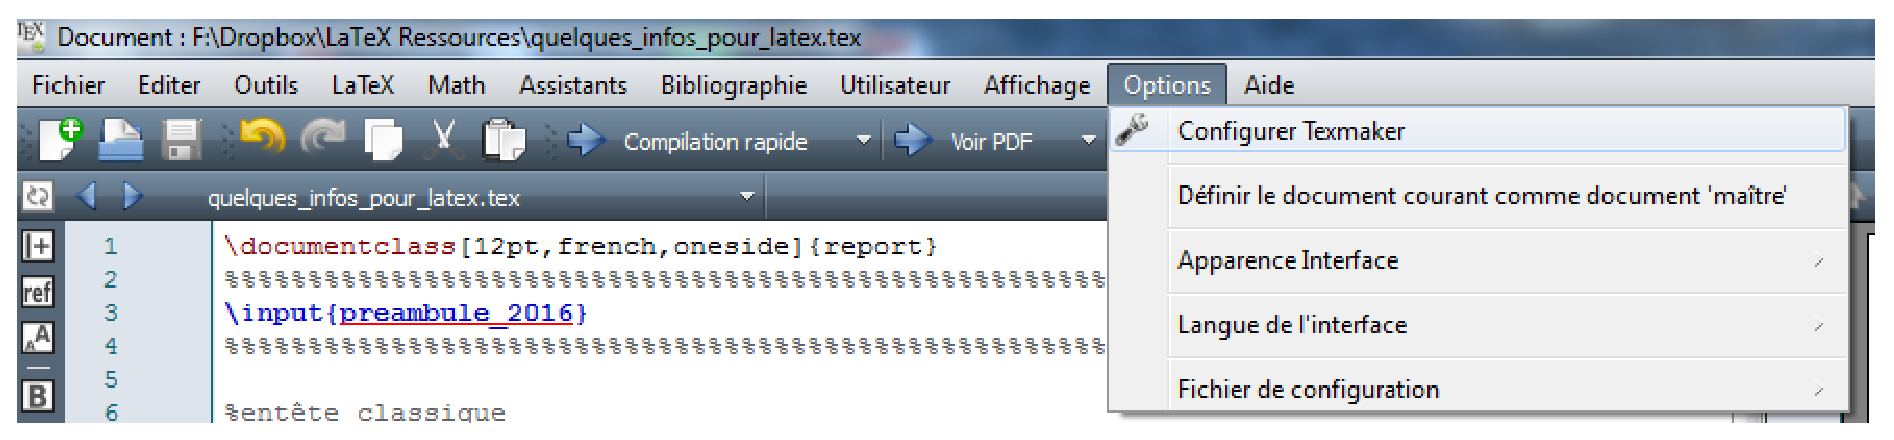
\includegraphics[width=0.8\textwidth]{installation/Capture1}
\end{center}

$\star$ On affiche l'écran suivant en choisissant \og Commandes \fg{} dans la barre gauche de la fenêtre qui vient de s'ouvrir.

On clique ensuite sur \og Afficher Pdf interne \fg{} et on coche \og Intégré à la fenêtre \fg{} :

\begin{center}
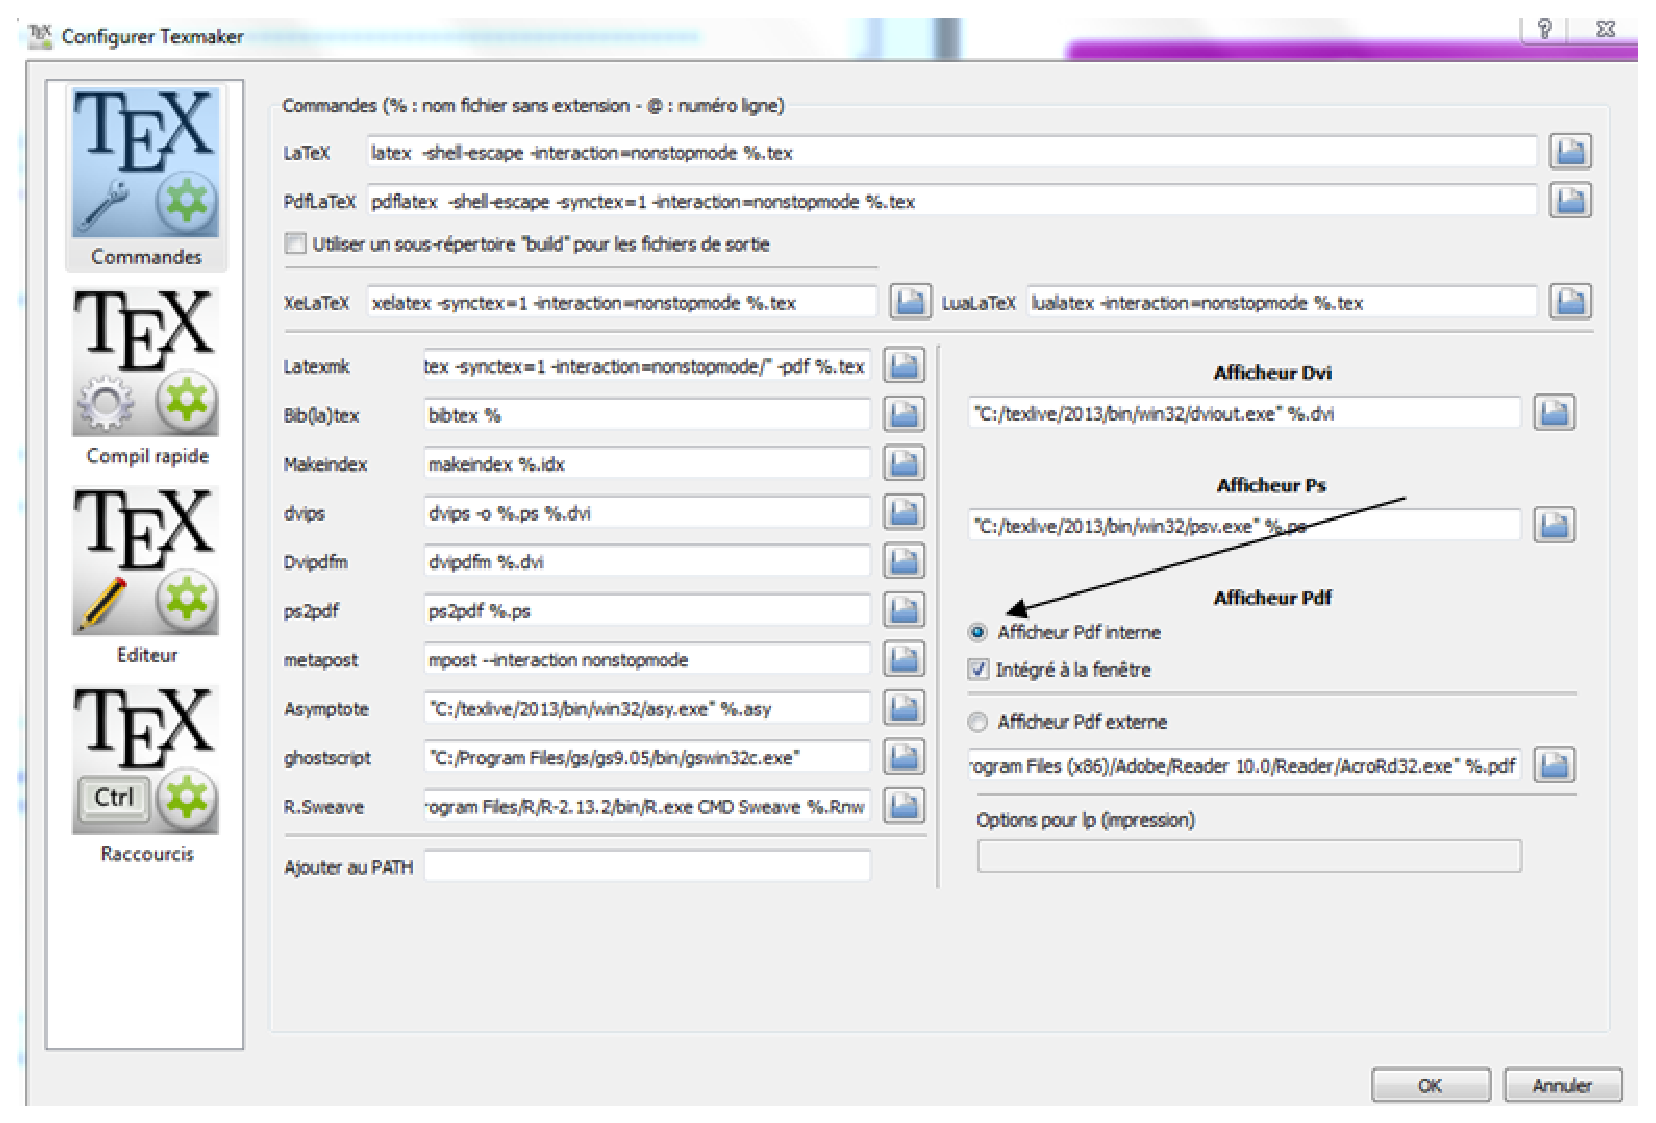
\includegraphics[width=0.8\textwidth]{installation/Capture2}
\end{center}

On valide en cliquant sur OK.

$\star$ Il suffit, pour terminer, de cocher sur \og Pdf Viewer\fg{} en bas à gauche :

\begin{center}
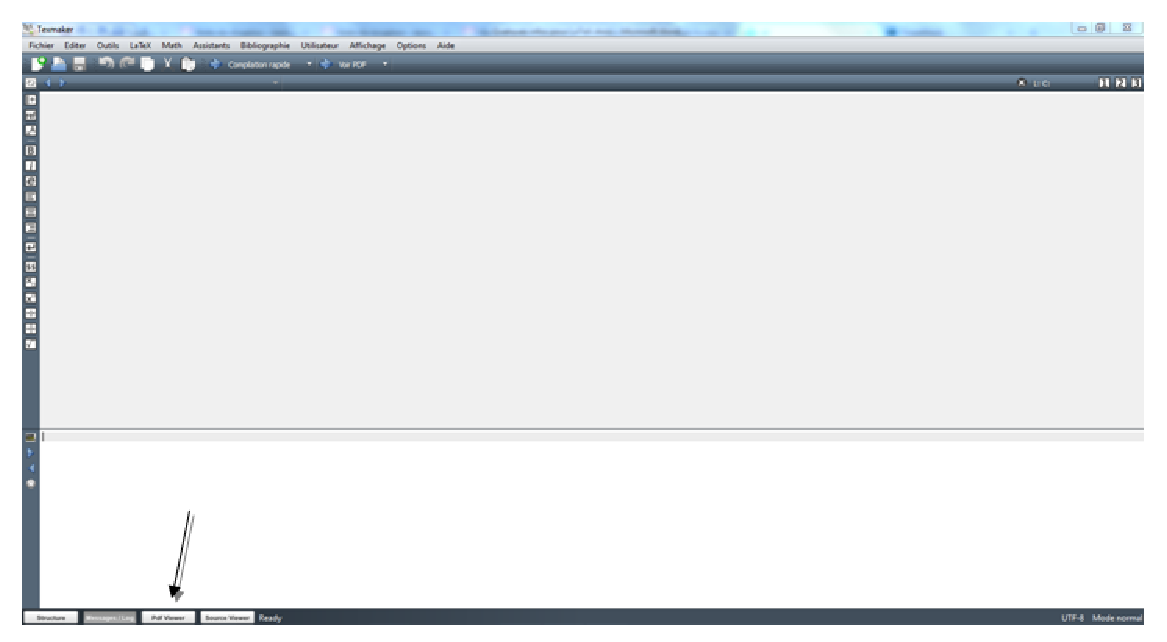
\includegraphics[width=0.8\textwidth]{installation/Capture}
\end{center}

\section{Personnalisation de TexMaker}

$\star$ Dans le menu \og Utilisateur\fg{},

\begin{itemize}

\item on peut créer des balises,

\item ajouter des commandes,

\item ajouter des termes au \og dictionnaire\fg{} initial reconnu par le logiciel qu'il utilise pour effectuer de l'auto-complétion.

\end{itemize}

$\star$ Dans le menu \og Options \fg{}, en cliquant sur\og Configurer Texmaker \fg{}, 

\begin{itemize}
\item on peut choisir le système d'encodage de l'éditeur

\begin{center}
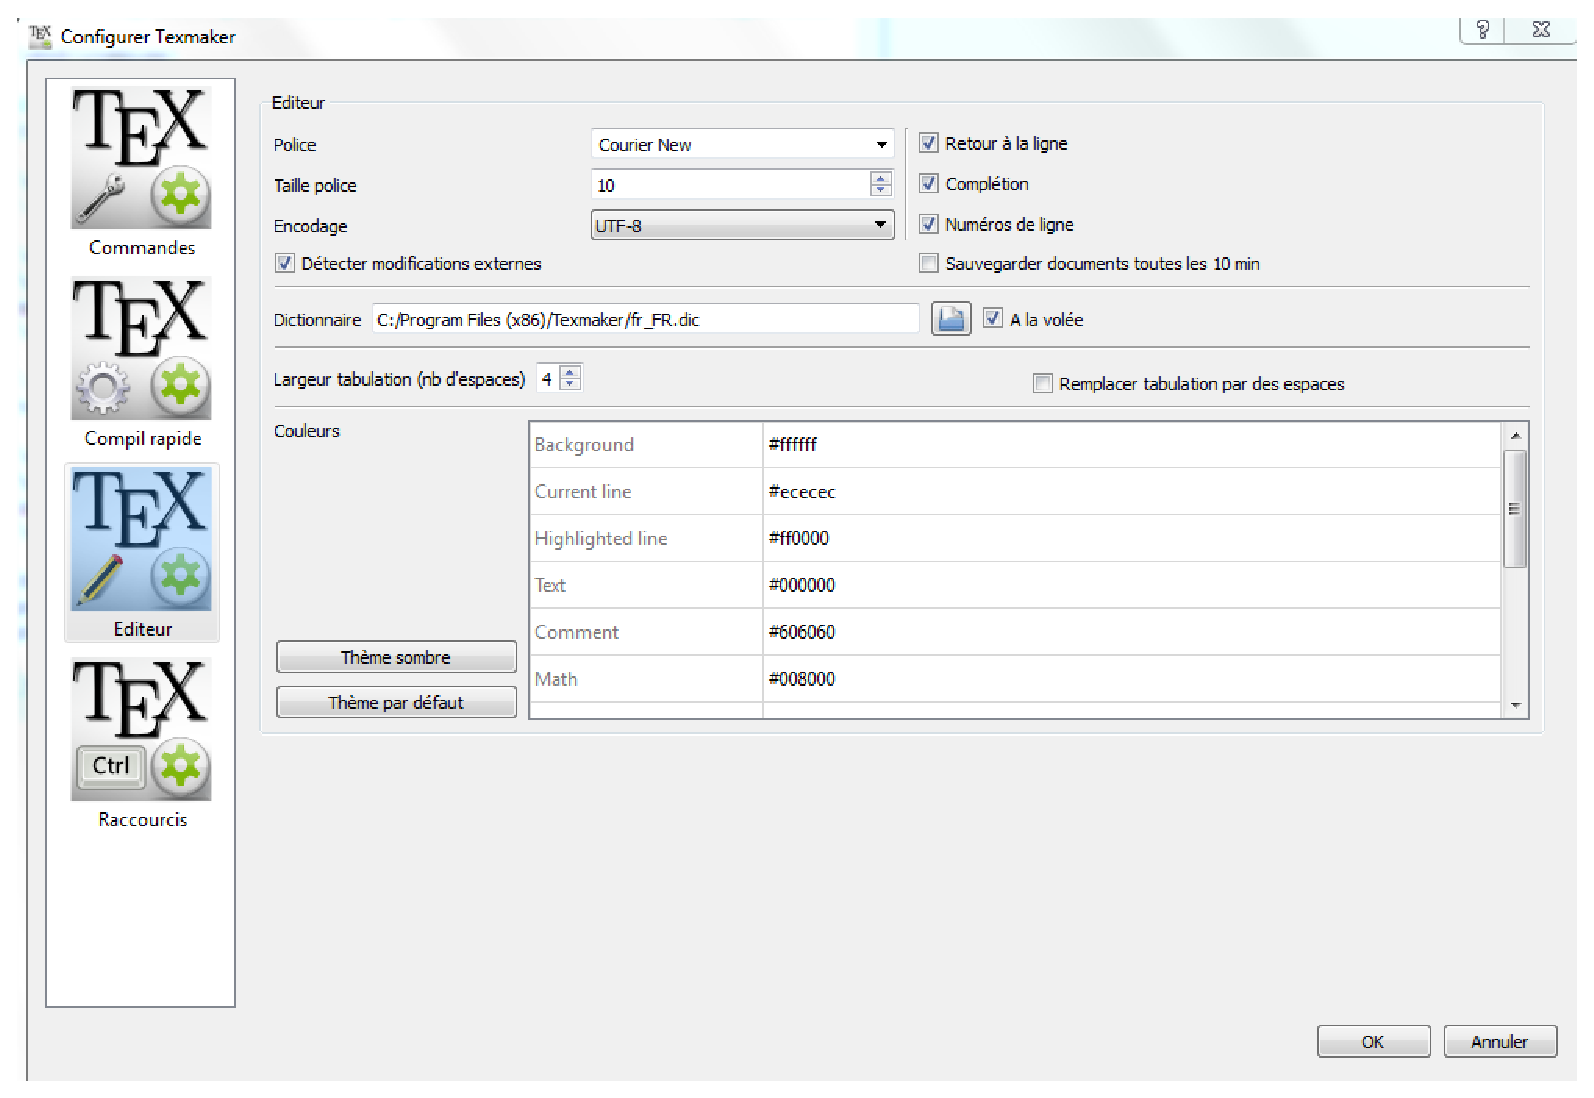
\includegraphics[width=0.5\linewidth]{installation/editeur_texmaker}
\end{center}

\item ainsi que la méthode de compilation (accessible par la touche \touche{F1})

\begin{center}
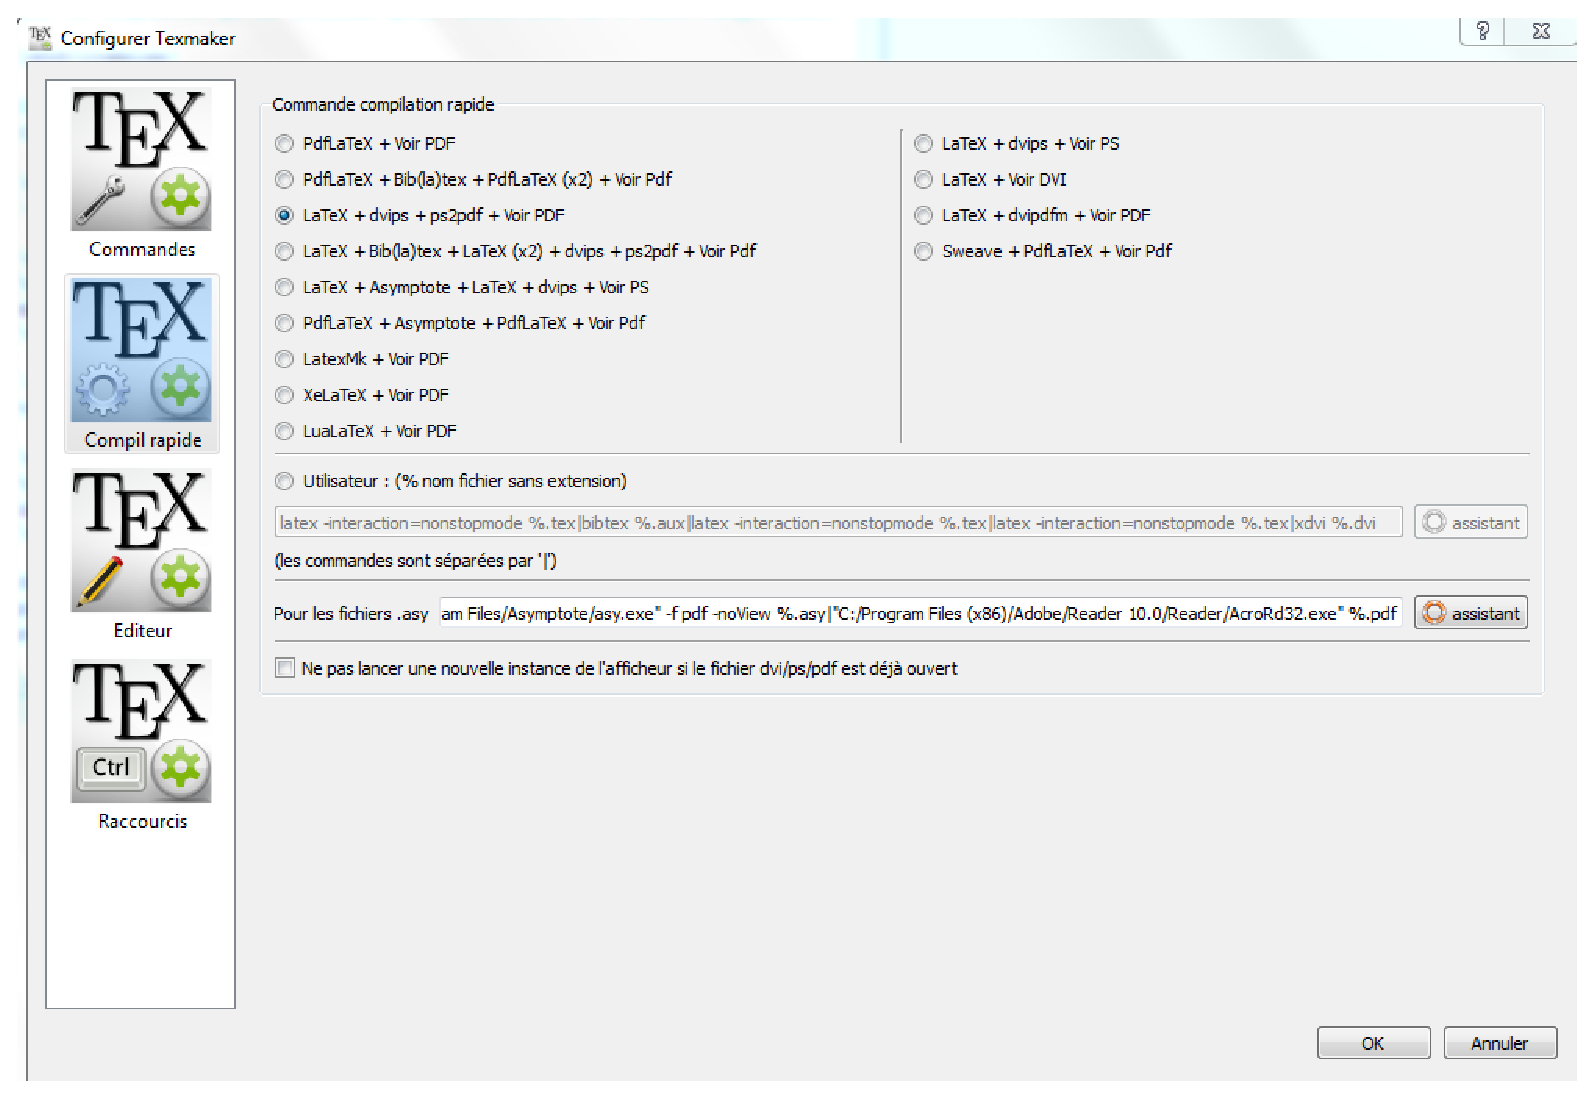
\includegraphics[width=0.5\linewidth]{installation/compil_texmaker}
\end{center}

Si le document final doit contenir des figures PSTricks et TikZ, préférez la méthode de compilation de la capture d'écran précédente.

\end{itemize}

\section{Installer un nouveau package non présent dans la distribution}

\subsection{\og À la main \fg{} }

Il existe plusieurs méthodes d'installation d'un  package avec LaTeX. J'ai sélectionné pour vous les deux plus faciles à mon sens. Elles devraient vous permettre d'utiliser la quasi-totalité des packages.

Les deux méthodes développées ici diffèrent légèrement, suivant que votre package est un fichier .ins ou .sty.

Dans de rares cas, les packages sont fournis sous d'autres extensions, mais ils sont alors accompagnés d'un fichier README vous guidant lors de leur installation.

\subsubsection{Les packages en .sty, méthode simple}

Si votre \jargon{package} est de la forme \verb~nom_de_package.sty~, rien de plus simple pour l'utiliser : il suffit de le copier dans le dossier contenant votre source .tex. Lorsque votre distribution compilera le fichier .tex, elle recherchera dans ce dossier les fichiers .sty des packages manquants, et le tour sera joué.

Résumons, la commande \verb~\usepackage{nom_de_package}~ demande à LaTeX d'utiliser un \jargon{package} installé ou, s'il ne l'est pas, d'aller chercher le fichier \verb~nom_de_package.sty~ dans le dossier de travail.

Simple, n'est-ce pas ?

Mais si l'on veut pouvoir réutiliser ce même \jargon{package} pour d'autres documents sans avoir à la copier dans le dossier de travail, on le copiera dans le dossier du PC contenant tous les \jargon{packages} :

\begin{enumerate}
\item Sur mon installation, il s'agit du répertoire :

\begin{enumerate}
\item \verb~C:\texlive\2013\texmf-dist\tex\latex~ pour mon pc sous Windows 7

\item \verb~/usr/local/texlive/2013/texmf-dist/tex/latex~ pour mon netbook sous Linux

\end{enumerate}

\item Il faut ensuite demander à la distribution installée de prendre en compte cet ajout :

\begin{enumerate}
\item Sous Windows

Lancer \og Tex Live Manager\fg{}, puis dans le menu \og Actions\fg{}, cliquer sur \og Update filename database\fg{}

OU

Lancer l'invite de commandes et taper \og texhash\fg{} (sans les guillemets\dots), puis valider.

\item Sous Linux

Lancer un terminal en administrateur et taper \og texhash\fg{} (sans les guillemets), puis valider.

\end{enumerate}

\end{enumerate}

\subsubsection{Les packages en .ins, méthode en deux temps}

Les \jargon{packages} contenus dans un fichier .ins doivent être traités en deux étapes. 

Premièrement, mettez votre fichier \verb~nom_de_package.ins~ dans un répertoire et compilez-le (c'est-à-dire, lancer la commande \verb~latex nom_de_package.ins~ en ligne de commandes) : il génèrera un fichier \verb~nom_de_package.sty~.

Ce fichier \verb~nom_de_package.sty~ doit être traité selon le processus développé dans le paragraphe \og Les packages en .sty, méthode simple \fg{}.



\subsection{Vérifier si un package est présent dans la distribution avec TeX Live Manager}

On lance Tex Live Manager et on voit alors apparaître la liste de tous les \jargon{packages} présents dans la distribution.

\begin{center}
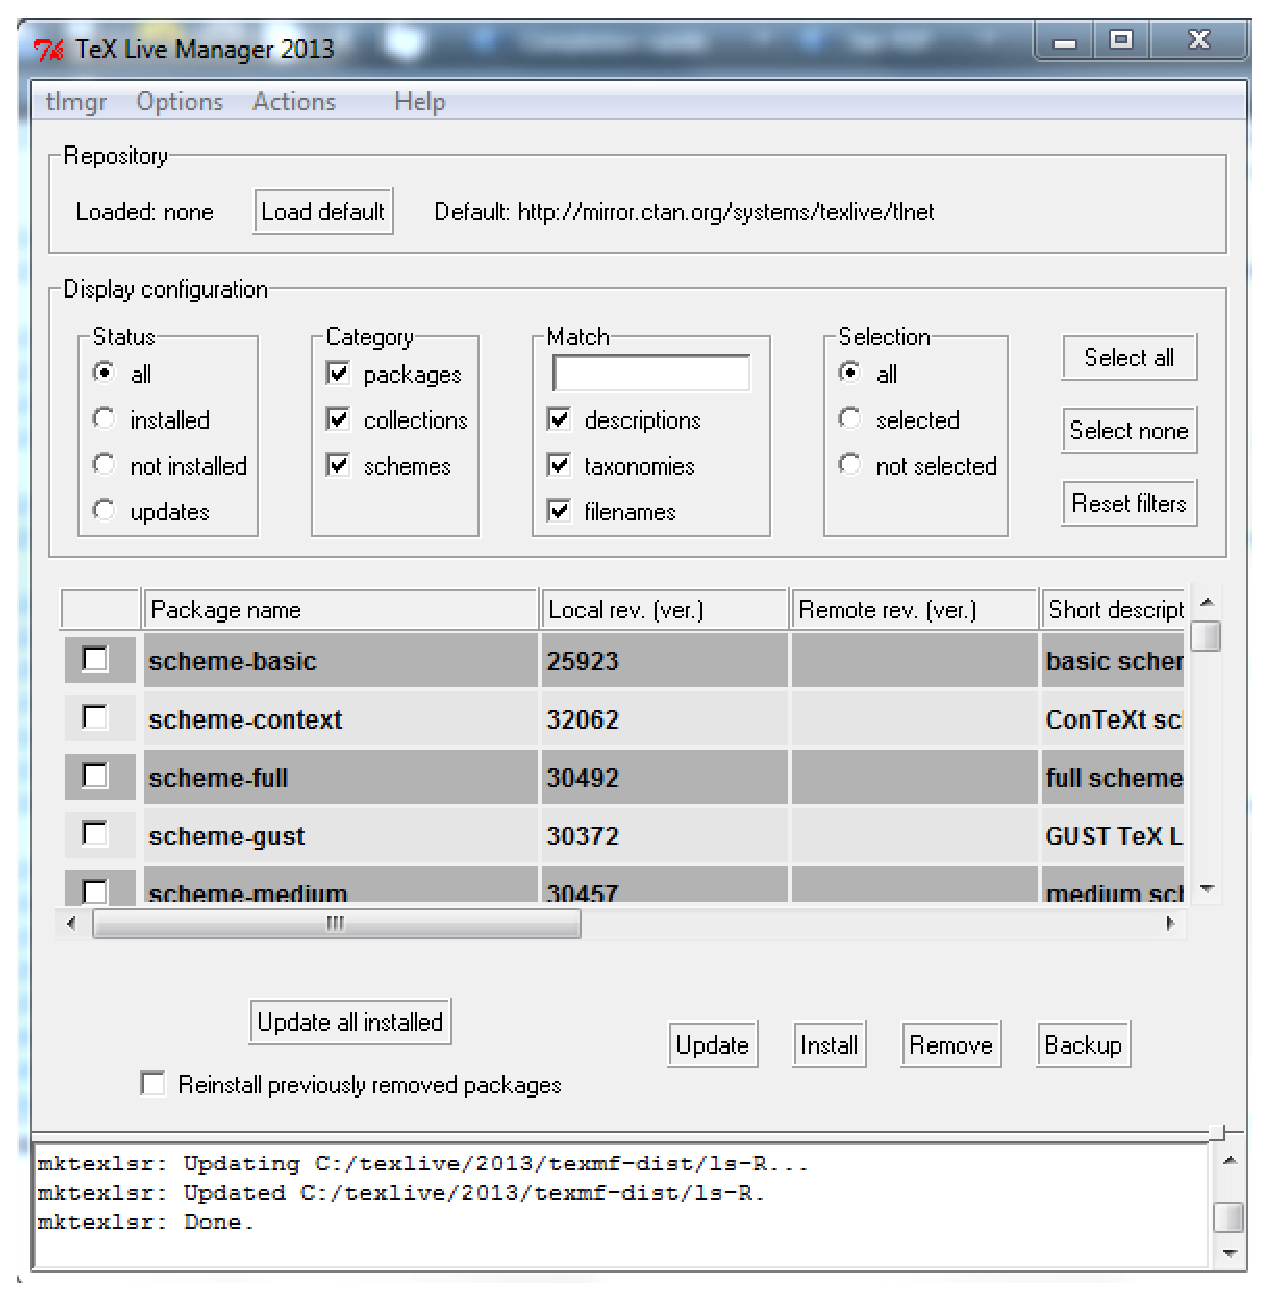
\includegraphics[width=0.6\textwidth]{installation/Capture3}
\end{center}


On peut également utiliser la ligne \og Match \fg{} en tapant les premières lettres du nom de \jargon{package} cherché pour accélérer la recherche.

\section{Sites sur lesquels on trouve des documents écrits avec \LaTeX}

$\star$ Parmi les sites sur lesquels on trouve des exercices de Mathématiques écrits avec \LaTeX, on peut citer \href{http://www.sesamath.net/}{Sesamath} dont les manuels pour le lycée utilisent \LaTeX, ou l'incontournable site de l'\href{http://www.apmep.fr/}{APMEP} avec sa section de sujets d'annales pour le brevet, le bac, le bts etc.

$\star$ Et parmi les très nombreux sites sur lesquels on trouve de la documentation sur l'utilisation de \LaTeX{} orientée \og Mathématiques \fg{}, on peut citer :

\begin{itemize}
\item la \href{http://math.univ-lyon1.fr/irem/spip.php?article340}{section dédiée} sur le site de l'Irem de l'académie de Lyon qui contient une brochure intitulée \og 	
LaTeX\dots pour le prof de maths ! \fg{} ,

\item le site \href{http://www.xm1math.net/}{xm1math} de Pascal Brachet (déjà cité plus tôt),

\item le site \href{http://math.et.info.free.fr/}{math.et.info} avec sa rubrique sur TikZ (très utile pour les figures et graphiques (voir le chapitre \ref{graph})),

\item le site \href{http://altermundus.fr/}{altermundus} qui contient de l'aide pour l'utilisation de TikZ et TkZ pour les graphiques et figures (voir le chapitre \ref{graph}),

\item et le site \href{http://www.texample.net/tikz/examples/}{texample.net} sur lequel on retrouve énormément de figures créées avec TikZ.

\end{itemize}


\section{Logiciels ou sites permettant d'extraire du code \LaTeX}

$\star$ Certains logiciels permettent d'exporter dans un format utilisable par \LaTeX{} les graphiques créés.

C'est le cas d'\textbf{Algobox}, de \textbf{Geogebra}, de \textbf{PdfAdd}, qui permet de créer les graphiques ci-dessous, en générant du code Asymptote (ou \LaTeX{} pour les tableaux de variations/signes) qu'il suffit de copier/coller dans son document \LaTeX{} :

\begin{center}
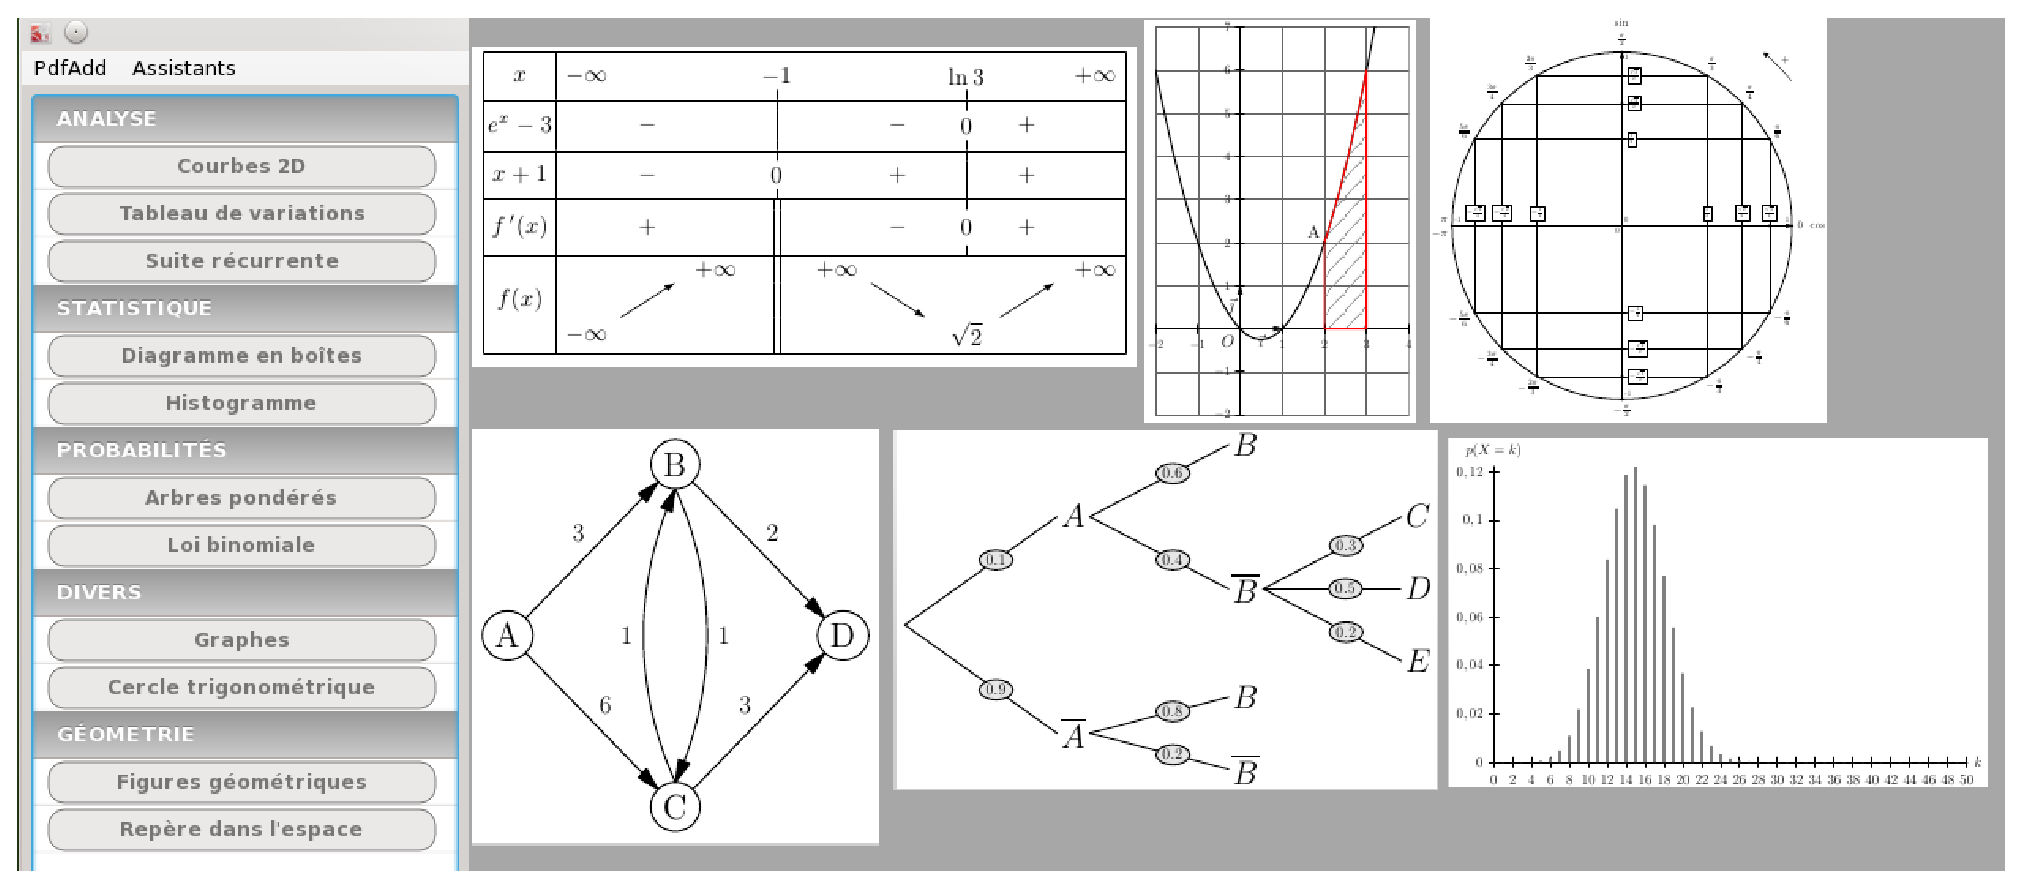
\includegraphics[width=0.7\textwidth]{installation/pdfadd}
\end{center}

C'est également le cas de \textbf{Pst+}, qui permet de créer les graphiques ci-dessous, en générant du code \LaTeX/PSTricks qu'il suffit de copier/coller dans son document \LaTeX{} :

\begin{center}
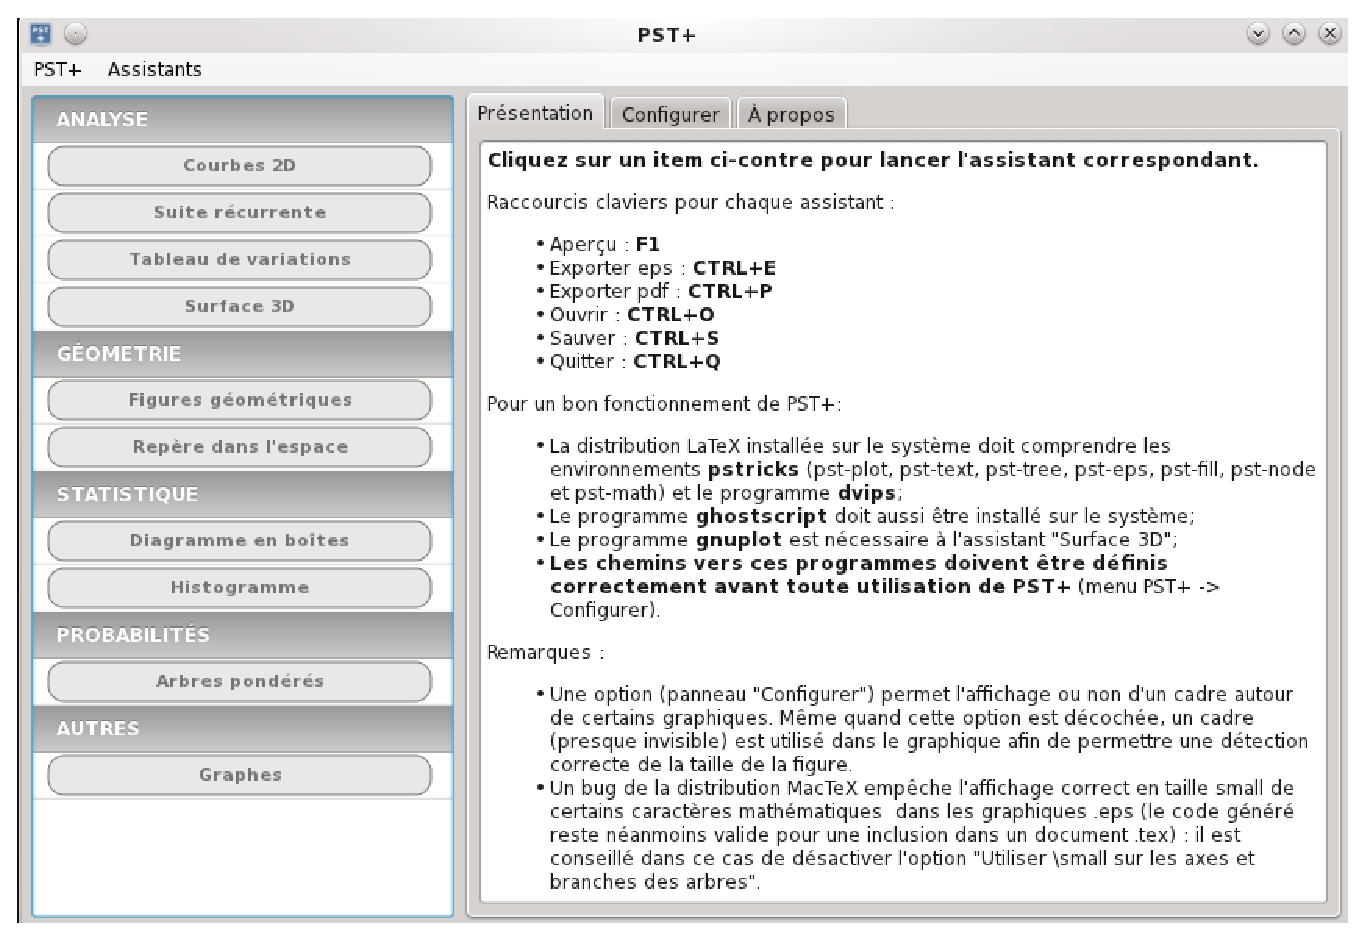
\includegraphics[width=0.7\textwidth]{installation/pstplus}
\end{center}

$\star$ On peut également intégrer du code \LaTeX{} dans la plupart des blogs, ou directement dans une zone graphique du logiciel \textbf{Geogebra}.

$\star$ Sur le site \href{http://math.et.info.free.fr/}{math.et.info}, on peut créer des tableaux de variations et des arbres pondérés, puis récupérer le code TikZ à copier/coller dans le document \LaTeX{}.

\chapter{Premier document}

\section{Mon premier document \LaTeX{}}
\subsection{\'Ecrire un fichier source}

Dans la pratique, ce que l'on écrit avec \jargon{Texmaker} se nomme le \jargon{fichier source} (ou encore le \jargon{code source}). Ce fichier est compilé par \LaTeX{} (plusieurs fois si nécessaire) et les différentes lignes de code sont interprétées pour obtenir en bout de chaîne le document final, celui qui sera imprimé.\medskip

Voici un premier document que vous pouvez taper dans votre éditeur, enregistrer, puis compiler (touche \touche{F1} sur \jargon{TeXmaker}).

\VerbatimInput[label={[Premier document]},gobble=0]{exemples/PremierDoc.tex}

\begin{info}
En règle générale, dans les noms des documents, on évitera d'utiliser des espaces et des lettres accentuées.
\end{info}


\subsection{Premières remarques}

\begin{enumerate}
    \item Le symbole \ordi{\$} sert à ouvrir et fermer le mode mathématiques (qui permet d'écrire des formules mathématiques).
    \item Le symbole \ordi{\%} permet d'écrire des commentaires qui n'apparaîtront pas dans le document compilé.
    \item La commande \verb!\par! de la ligne 10 sert à effectuer un saut de ligne dans le document compilé.
    
    Une ligne vide a le même effet.
    
    Personnellement, je préfère la deuxième solution qui me permet d'aérer mon \jargon{code source}.
    
    \item Un simple changement de ligne dans le \jargon{code source} ne sert qu'à aérer le \jargon{code source} et n'a aucun effet sur le document final.
    \item Dans le \jargon{code source}, lorsque plusieurs espaces séparent deux mots, \LaTeX{} n'en prend qu'un seul en compte.
\end{enumerate}

\section{Explication rapide du code source}
\subsection{Structure du code source}

Le code source est divisé en plusieurs parties :
\begin{description}
    \item[La définition du document :] la première ligne permet de déterminer quel type de document est réalisé : on parle de la \jargon{classe} du document (d'où le nom \verb!documentclass!). 
    
    Ici, il s'agit d'un document de type \verb!article!. Les \jargon{options globales} sont également déterminées à ce moment : elles sont valables pour tout le document sauf indication contraire.
    \item[Le préambule :] il s'agit des lignes entre \textbackslash\verb!documentclass! et \verb!\begin{document}! (lignes 2 à 8). 
    
    Le préambule contient tous les package(s) utilisés ainsi que différentes \jargon{commandes} définies par l'utilisateur ou spécifiquement utilisées dans le préambule.
    \item[Le corps du document :] situé entre \verb!\begin{document}! et \verb!\end{document}!,
        il s'agit du contenu même du document qui sera alors formaté en fonction du contenu du préambule et des commandes utilisées dans le texte.
    \item[Après :] les lignes après \verb!\end{document}!
        ne sont pas interprétées par \LaTeX{} et peuvent donc contenir ce que l'on veut : des commentaires, des notes, des parties mises de côté\dots
\end{description}

\subsection{Explication du préambule}

\begin{description}
    \item[] \verb!\documentclass[12pt,french]{article}! : cette commande indique que le document est de classe \verb!article! et sera donc assez court. Il existe, en comparaison, la classe \verb!book! pour écrire des documents plus longs. Bien d'autres classes existent (\verb!letter!, \verb!beamer!,\dots).\par
        Ce document respectera la typographie française et la taille des fontes sera de \verb!12pt! (\verb!10pt! étant la taille par défaut).
    \item[] \verb!\usepackage[utf8x]{inputenc}! : cette commande permet de charger le package \verb!inputenc! avec l'option \verb!utf8x!. Nous n'expliquerons rien en détails ici mais cela gère le \jargon{codage} d'entrée des caractères du \jargon{code source} (d'où l'intérêt d'avoir configuré \jargon{Texmaker} en \ordi{utf8}).
    \item[] \verb!\usepackage[T1]{fontenc}! : cette commande permet de charger le package \verb!fontenc! avec l'option \verb!T1! permettant de gérer, entre autre, les caractères accentués et notamment les \og copiés-collés \fg{} à partir de fichiers \bsc{pdf}.
    \item[] \verb!\usepackage[upright]{fourier}! : charge le package \verb!fourier! avec son option \verb!upright! qui permet d'avoir d'avoir les majuscules droites dans les formules mathématiques.
   % \item[] \verb!\usepackage{kpfonts}! : charge un ensemble de fontes de la police \jargon{Kp-Fonts}. D'autres sont disponibles comme par exemple \verb!mathpazo! pour la police \jargon{Palatino} ou bien \verb!mathptmx! pour la police \jargon{Times}.
    \item[] \verb!\usepackage[a4paper,margin=2cm]{geometry}! : charge le package \verb!geometry! avec différentes options de mise en page.
    \item[] \verb!\usepackage{mathtools,amssymb}! : charge le package \verb!mathtools! qui est essentiel dans un document destiné à composer des textes scientifiques, avec un formalisme et donc une mise en page particulière. Le package \verb!amssymb! regroupe quant à lui quantité de symboles utilisés notamment en mathématiques et en physiques.
    \item[] \verb!\usepackage{babel}! : obligatoirement le dernier de la liste. Le package \verb!babel! permet d'assurer au rédacteur que le texte sera composé en respectant les usages propres à la langue de composition du document (ici en français). La langue peut être spécifiée en option de ce package en écrivant \verb!\usepackage[french]{babel}! mais il est préférable d'indiquer l'option de langue avec la \jargon{classe} du document (comme nous l'avons fait). Ainsi, cette langue sera utilisée de façon globale par tous les package(s) en ayant besoin.
\end{description}

\section{Commandes}
\subsection{Arguments d'une commande}
Les \jargon{commandes} permettent de structurer et de mettre en forme le document. Elles sont reconnaissables car elles commencent par le caractère \textbackslash{} suivi du nom de la commande (plus ou moins explicite). La commande se termine par tout caractère autre qu'une lettre (accolade, crochet, chiffre, espace, ponctuation\dots).\par

Différents types de commandes existent :
\begin{description}
    \item[Sans \jargon{paramètres} :] elles exécutent simplement une action : \verb!\neq!, \verb!\par!, \verb!\Leftrightarrow!
    \item[Avec \jargon{paramètres} :] il existe alors deux types de \jargon{paramètres}. Ils peuvent être :
        \begin{description}
            \item[Obligatoires :] ceux-là sont notés entre accolades et il peut y avoir plusieurs paramètres par commande (une paire d'accolades pour chacun d'entre eux). Par exemple, la commande \verb!\textbf! ne possède qu'un paramètre alors que la commande \verb!\frac! en possède deux. Il a été dit que la commande s'arrêtait par tout caractère autre qu'une lettre. 
            
Dans ce cas, il n'est pas toujours nécessaire d'utiliser les accolades. 

Ainsi, \verb!\frac{2}{3}! $\qLRq$ \verb!\frac23! $\qLRq$ \verb!\frac 2 3 ! : cela donne la fraction $\textstyle \frac23$. 

En revanche, écrire \verb!\fracab! ne donnera pas $\textstyle \frac a b$, car \LaTeX{} ne saura pas interpréter la commande \verb!\fracab! (à moins que vous ayez créé une commande portant ce nom).

            \item[Facultatifs :] ceux-là sont notés entre crochets avant le premier argument obligatoire (qui n'existe pas toujours d'ailleurs). Les \jargon{arguments} facultatifs ou \jargon{optionnels} permettent de modifier localement l'action d'une commande. Par exemple \verb!\sqrt[3]{x}!.
        \end{description}
\end{description}

En résumé, une commande peut avoir une des trois formes suivantes :

	\verb!\commande! \par
	\verb!\commande!\{<\verb!argument 1!>\}\{<\verb!argument 2!>\}\dots\par
	\verb!\commande![<\verb!argument optionnel!>]\{<\verb!argument 1!>\}\{<\verb!argument 2!>\}\dots


\begin{info}
    Les majuscules dans les noms de commandes sont importantes : ainsi \ordi{\textbackslash frac} n'est pas identique à \ordi{\textbackslash Frac}.
\end{info}

\subsection{Commandes semi-globales}

Les \jargon{commandes locales} permettent de modifier l'aspect du texte de façon locale.\par
Les \jargon{commandes semi-globales} n'ont pas d'argument et modifient tout le texte qui suit jusqu'à ce qu'une autre commande semi-globale ou qu'une commande locale ne modifie encore la mise en forme. On peut limiter l'action des commandes semi-globales à l'aide d'une paire d'accolades englobant le texte mais également la commande. Autrement dit :
\begin{description}
    \item[Commande locale :] \verb!\commande!\{<du texte>\}
    \item[Commande semi-globale :] \verb!{!\verb!\commande! <du texte>\verb!}!
\end{description}

La plupart du temps, on utilise les commandes locales sur des textes courts sans changement de paragraphes alors que les commandes semi-globales sont appliquées à des textes plus longs et acceptent les changements de paragraphes. Voici un exemple :\bigskip

\begin{SideBySideExample}
    Voici un \textbf{exemple :}
    tout va bien mais on peut vouloir
    continuer avec un texte
    \tiny plus petit jusqu'au bout.\par
    {\bfseries
        Cela est important !\par
        Comprenez-vous ?
    }
    C'est bien !
\end{SideBySideExample}


\subsection{Les packages}

Les package(s) sont chargés à l'aide de la commande \verb!\usepackage!. Chaque package est une \jargon{extension} de \LaTeX{} et c'est la création de ces milliers de package(s) qui fait que \LaTeX{} évolue de jours en jours. Le nom du package est l'argument obligatoire et les options sont spécifiées entre crochets si nécessaire :
\begin{center}
    \verb!\usepackage![<\verb!options!>]\{<\verb!nom du package!>\}
\end{center}
Si plusieurs package(s) doivent être appelés sans option particulière (ou avec la même option), alors on peut les lister au sein de la même commande \verb!\usepackage!. C'est le cas par exemple de la ligne 4 : \verb!\usepackage{mathtools,amssymb}! fait appel à deux package(s) liés aux mathématiques.

\begin{info}
    \textbf{Rappel :} Le package \verb!babel! est le package qui permet la gestion de la langue dans laquelle est écrite le document. C'est d'ailleurs la fonctionnalité de \verb!french! signalée dans la \jargon{commande} \textbackslash\verb!documentclass!.\par
    Le package \verb!babel! doit être, en général, le dernier de la liste des package(s) utilisés.
\end{info}

\section{Les caractères spéciaux}

On a vu que certains caractères avaient une utilisation spécifique dans le code source : c'est le cas par exemple des caractères \ordi{\%} et \ordi{\$} qui permettent respectivement d'entrer un commentaire et une formule mathématique. Comment faire cependant pour écrire -20\% sur une veste à 50\$ ou bien $S = \{ 1 ; 3 \}$ ?\par
Le \og texte\fg{} ci-dessous donne les caractères spéciaux réservés par \LaTeX{} et la syntaxe nécessaire pour les utiliser dans un texte classique :

Voici quelques exemples de caractères spéciaux, réservés par \LaTeX{} :

\verb!\{! et \verb!\}!, utiles pour les ensembles, donnent les accolades ouvrante et fermante,

\verb!%! qui sert à écrire des commentaires dans le code source

\verb!$! qui sert à ouvrir ou fermer le mode \og mathématiques\fg{}

\verb!^! qui sert pour les exposants

\verb!_! qui sert pour les indices

\verb!&! qui sert pour les tableaux (séparateur de colonnes)

\verb!#! qui sert lorsque l'on définit des commandes personnelles

\verb!~! qui produit un espace insécable


\begin{info}
	Le caractère \verb!@! n'est pas un caractère spécial et permet d'obtenir simplement @.\par
	Cependant, dans certains cas, il est utilisé de façon particulière : pour les tableaux, les commandes personnelles...
\end{info}



\chapter{Mise en forme}

\section{Mise en forme de base}

\subsection{Un premier exemple}

Recopier et compiler le \jargon{code source} suivant :

%\VerbatimInput[label={[Quelques mises en forme]\NumCode},gobble=0]{exemples/mise_en_forme.tex}
\VerbatimInput[label={[Quelques mises en forme]},gobble=0]{exemples/mise_en_forme.tex}

\begin{enumerate}
    \item Nommer cinq différentes mises en forme utilisées dans ce document.
    \item Quelle(s) commandes permettent d'obtenir ces mises en forme ?
    \item Quelle(s) différence(s) y a-t-il entre les deux commandes qui permettent de mettre du texte en gras ?
\end{enumerate}


\subsection{Police et fontes}

Une \jargon{police} se déclinent en trois caractéristiques : famille, formes et graisses qui constituent alors un ensemble de \jargon{fontes} de cette police. Le tableau ci-dessous résume les commandes permettant d'utiliser une de ces fontes.

\begin{info}
	Le caractère $\sqcup$ indique qu'il faut laisser un espace dans le \jargon{code source}.
\end{info}

\begin{center}
    \begin{tabular}{|>\bfseries cl|c|c|l|}
    \cline{3-5}
        \multicolumn{2}{c|}{} & \multicolumn{2}{c|}{Portée} & \multicolumn{1}{c|}{Signification} \\
        \multicolumn{2}{c|}{} & locale & semi-globale & \multicolumn{1}{c|}{des radicaux} \\
    \hline
        \multirow{3}*{Familles} & romain (par défaut) & \verb!\textrm!\{<texte>\} & \verb*!\rmfamily !<texte> & \verb!rm! = roman\\
    \cline{2-5}
        & {\sffamily sans empattement} & \verb!\textsf!\{<texte>\} & \verb*!\sffamily !<texte> & \verb!sf! = sans serif \\
    \cline{2-5}
        & {\ttfamily à chasse fixe} & \verb!\texttt!\{<texte>\} & \verb*!\ttfamily !<texte> & \verb!tt! = teletype \\
    \hline\hline
        \multirow{4}*{Formes} & droit (par défaut) & \verb!\textup!\{<texte>\} & \verb*!\upshape !<texte> & \verb!up! = upright (droit)\\
      \cline{2-5}
        & \textsl{incliné} & \verb!\textsl!\{<texte>\} & \verb*!\slshape !<texte> & \verb!sl! = slanted (penché) \\
      \cline{2-5}
        & \textit{italique} & \verb!\textit!\{<texte>\} & \verb*!\itshape !<texte> & \verb!it! = italique \\
      \cline{2-5}
        & \textsc{petites capitales} & \verb!\textsc!\{<texte>\} & \verb*!\scshape !<texte> & \verb!sc! = small caps \\
    \hline\hline
        \multirow{2}*{Graisses} & médium (par défaut) & \verb!\textmd!\{<texte>\} & \verb*!\mdseries !<texte> & \verb!ms! = medium\\
      \cline{2-5}
        & \textbf{gras} & \verb!\textbf!\{<texte>\} & \verb*!\bfseries !<texte> & \verb!bf! = bold face (gras) \\
    \hline
    \end{tabular}
\end{center}

\begin{info}
    Plusieurs commandes peuvent être utilisées conjointement. 
    
    Par exemple pour obtenir du texte en \textit{\textbf{gras, italique et sans empattement}}, on écrira :\par

    \texttt{\textbackslash textsf
    \hspace*{-6pt}\{\hspace*{-6pt}
    \textbackslash textbf
    \hspace*{-6pt}\{\hspace*{-6pt}
    \textbackslash textit
    \hspace*{-6pt}\{\hspace*{-6pt}
    <texte>
    \hspace*{-6pt}\}\}\}
    }

    L'ordre des commandes n'a pas d'importance mais il faut faire attention à avoir le bon nombre de paires d'accolades.
\end{info}

\subsection{Changement de la taille des fontes}

La taille des fontes peut être fixée de manière absolue dans le préambule, en option à \textbackslash\verb!documentclass!. Les options disponibles sont \verb!10pt! (valeur par défaut si rien n'est indiqué), \verb!11pt! et \verb!12pt!.\par
Une fois définie cette taille absolue, on peut agrandir et réduire la taille d'une partie du document en utilisant des \jargon{commandes semi-globales} qui modifient alors le texte de façon relative. Le changement dépendra en effet de la taille absolue. Ces commandes sont les suivantes :
\begin{center}
	\begin{tabular}{ll}
		\hline
		Commande & Signification et test \\
		\hline
			\verb*!\tiny <texte>! & {\tiny minuscule}\\
			\verb*!\scriptsize <texte>! & {\scriptsize taille des indices et exposants}\\
			\verb*!\footnotesize <texte>! & {\footnotesize Taille des notes de bas de pages}\\
			\verb*!\small <texte>! & {\small petit}\\
			\verb*!\normalsize <texte>! & taille définie par l'option absolue\\
			\verb*!\large <texte>! & {\large grand}\\
			\verb*!\Large <texte>! & {\Large plus grand}\\
			\verb*!\LARGE <texte>! & {\LARGE encore plus grand}\\
			\verb*!\huge <texte>! & {\huge énorme}\\
			\verb*!\Huge <texte>! & {\Huge encore plus énorme}\\
		\hline
	\end{tabular}
\end{center}

\begin{info}
	Les majuscules dans le nom des commandes sont importantes.\par
	De plus, il s'agit de commandes \jargon{semi-globales} donc il faut penser à mettre des accolades englobantes si on veut modifier la taille d'une partie du texte seulement.
\end{info}


\subsection{Alignement}

Par défaut, le texte est \jargon{justifié}. Cela signifie que \LaTeX{} gère les espaces entre les mots pour que le texte soit aligné à gauche \textbf{et} à droite.\par
Cependant, on peut parfois avoir besoin de centrer le texte, ou bien de demander uniquement un alignement à gauche ou uniquement un alignement à droite. Pour cela, on utilise respectivement les \jargon{environnements} \ordi{center}, \ordi{flushleft}, \ordi{flushright}.\bigskip

{
\begin{SideBySideExample}
    \begin{center}
    Du texte au centre.
    \end{center}
    \begin{flushleft}
    Alignement sur la gauche.
    \end{flushleft}
    \begin{flushright}
    Alignement sur la droite.
    \end{flushright}
\end{SideBySideExample}
}

\begin{info}
    \textbackslash \verb!centering! est la commande semi-globale associé à l'environnement \ordi{center}. \textbackslash \verb!raggedleft! est associé à \ordi{flushright} et \textbackslash \verb!raggedright! est associée à \ordi{flushleft}.
\end{info}

\subsection{Espaces}

\begin{info}
    Les espaces écrits dans le \jargon{code source} ne sont pas identiquement restitués dans le document final après compilation.\par
    Pour cela, on parlera d'\textbf{un} espace dans le \jargon{fichier source} et d'\textbf{une} espace dans le document final.
\end{info}

\subsubsection{Espaces horizontales}

Nous l'avons vu précédemment, pour obtenir une espace entre deux mots, il suffit de saisir un espace dans le \jargon{code source} à l'aide de la barre d'espace du clavier. Cependant, saisir plusieurs espaces ne changera rien et lors de la compilation, ils seront interprétés comme un seul et même espace. De même pour un changement de ligne (sans ligne vide !) :\medskip

{
\begin{SideBySideExample}[showspaces=true]
    Du texte
        sur une
    seule          ligne.
\end{SideBySideExample}
}

\begin{info}
    Le symbole \ordi{\~{}} permet d'obtenir une \jargon{espace insécable}. En fin de ligne notamment, il faudra donc écrire \ordi{Louis\~{}XIV} si on veut éviter que \ordi{Louis} soit inscrit en bout de ligne et \ordi{XIV} au début de la ligne suivante.
\end{info}

Parfois, on peut avoir besoin d'une espace horizontale ayant une longueur bien précise. Cela est possible à l'aide de la commande \verb!\hspace!\{<longueur>\}. L'argument <longueur> est spécifié à l'aide d'un nombre suivi de son unité (sans espace entre les deux). L'unité peut être \ordi{cm}, \ordi{mm} ou bien encore \ordi{pt} mais bien d'autres aussi.\par
De plus, la commande \verb!\hfill! est un espace élastique. Voilà une façon de se servir de ces deux commandes :\bigskip

{
\begin{SideBySideExample}
    Les consignes sont vraiment importantes.\par
    Les consignes sont \hspace{1.4cm} vitales !\par
    Inutile \hspace{-1.3cm} xxxxxxx\par
    \textbf{Exercice 1} \hfill \textit{(2 points)}
\end{SideBySideExample}
\bigskip
}

\subsubsection{Espaces verticales}

Nous l'avons vu précédemment, pour changer de paragraphe, il suffit de saisir laisser une ligne vide dans le \jargon{code source}. La commande \verb!\par! assure la même fonction. Cependant, plusieurs lignes vides seront toujours interprétées comme un seul changement de paragraphe, de même que la succession de plusieurs commandes \verb!\par!.\par
Comment faire alors apparaître dans le document final des espaces entre deux paragraphes ?\par
La commande \verb!\vspace!\{<longueur>\} est une solution et cela fonctionne comme pour les espaces horizontales. Cependant, les commandes \verb!\smallskip!, \verb!\medskip! et \verb!\bigskip! sont simples et rapides à utiliser.\bigskip

{
\begin{SideBySideExample}
    Consigne importante.

    Espace standard.\smallskip



    Petite espace.\medskip

    Espace moyenne.\bigskip

    Grande espace.\par\vspace{2em}
    Espace personnelle.
\end{SideBySideExample}
\bigskip
}

Pour la commande \verb!\hspace{<longueur>}!, la longueur est un nombre avec une unité accolée, parmi :

$\star$ mm (millimètre) ;

$\star$ cm (centimètre) ;

$\star$ pt (point anglo-saxon) ;

$\star$ dd (point Didot) ;

$\star$ ex (hauteur d'x) ;

$\star$ em (cadratin).

Les unités ex et em sont proportionnelles au corps de la police :

$\star$ la hauteur d'x, parfois appelée à tort « hauteur d'œil », est la hauteur d'un bas de casse (lettre minuscule) sans hampe ni jambage, comme le x ;

$\star$ le cadratin est égal au corps de la police.

Par exemple :

$\star$ \verb!\hspace{1cm}! pour une espace de un centimètre ;

$\star$ \verb!\hspace{0.5em}! pour une espace d'un demi cadratin. 


\begin{info}
La commande \textbackslash \verb!vfill! permet de créer une espace verticale élastique. Essayer de compiler l'exemple ci-dessous.
\end{info}

\begin{Verbatim}
    Le devoir est sur 20 points.\par\vfill
    Tourner la page.
\end{Verbatim}

\section{Couleur}

\begin{info}
    Difficile de parler de couleurs sur des photocopies noir et blanc donc pensez à taper et compiler les exemples proposés.
\end{info}



Afin de colorer un document, on utilise le \jargon{package} \verb!xcolor!, chargé dans le préambule à l'aide de la commande \verb!\usepackage{xcolor}!. \verb!xcolor! permet d'accéder aux couleurs suivantes :
\begin{center}
    \ttfamily
    \begin{tabular}{*{7}{l}}
        red & magenta & gray & white & violet & olive & \\
        blue & cyan  & lightgray & black & purple & teal & brown \\
        green & yellow & darkgray & orange & pink & lime &
    \end{tabular}
\end{center}

Là encore, il existe une commande locale et une commande semi-globale dont voilà un exemple :\medskip

{
\begin{SideBySideExample}
    \color{blue}
    Les consignes suivantes sont
    \textcolor{red}{importantes.}\par
    Lisez-les avec \textit{attention}.\par
    Sinon, gare
    \textcolor{purple}{\textbf{\textsc{\`a vous}}} !
\end{SideBySideExample}
}

\begin{info}
    Le \jargon{package} \verb!xcolor! possède différentes options qui permettent d'accéder à bien d'autres couleurs. C'est le cas de l'option \verb!dvipsnames! qui donne accès à 68 couleurs en plus de celles de base. On écrira alors : \textbackslash\verb!usepackage!\texttt{[dvipsnames]\{xcolor\}} dans le préambule.\par
    La documentation du \jargon{package} permet d'en savoir davantage. Il suffit de taper sur un moteur de recherche \texttt{LaTeX xcolor doc} pour obtenir ce que l'on cherche.
\end{info}

Voilà un autre exemple qui montre comment faire des encadrements colorés.\bigskip

{
\begin{SideBySideExample}
    \begin{center}
        \colorbox{yellow}{\textbf{Chapitre 1 :}}\par
        \textit{L'art de faire des encadrements}
    \end{center}
    \fcolorbox{red}{lightgray}{\textbf{I. Partie 1}}
\end{SideBySideExample}
\bigskip}

Pour finir sur ce thème, voici la commande \textbackslash \verb!pagecolor{<couleur>}! qui permet de colorer le fond d'une page. Très utile pour créer un document destiné à être vidéoprojeté. En effet, le fond blanc d'un document projeté peut être fatigant pour les yeux des lecteurs. Allez-y : essayez !

\section{Mise en page}

\subsection{Dimensions de la page}

Par défaut, les dimensions de la page sont réglées en fonction de la \jargon{classe} du document.\par
Le \jargon{package} \verb!geometry! est utilisé pour régler la géométrie de la page indépendamment du choix de la \jargon{classe} : dimensions du papier, orientation (portrait, paysage), dimensions des marges, particularités d'un document recto-verso, dimensions des en-têtes et pieds-de-pages...

Pour cela, on peut charger le \jargon{package} avec toute une liste d'options séparées par une virgule :\par\medskip
\textbackslash\verb!usepackage[a4paper,margin=2cm]{geometry}!.\medskip

Il est également possible de charger le \jargon{package} tout seul puis d'utiliser la commande \verb!\geometry! qui prend en argument la même liste d'options. Ainsi, on peut également écrire :\par\medskip
\textbackslash\verb!usepackage{a4paper,geometry}!\par
\textbackslash\verb!geometry{margin=2cm}!\medskip

La documentation du \jargon{package} \verb!geometry! liste l'ensemble des options disponibles dont voici les plus courantes (<dim> est un nombre avec une unité de longueur) :
\begin{itemize}
    \item \verb!landscape! : orientation paysage ;
    \item \verb!twoside! : document recto-verso ;
    \item \verb!width=!<dim> et \verb!height=!<dim> : largeur et hauteur de la page. On peut aussi utiliser \verb!a4paper! ou \verb!a5paper! (formats disponibles de A0 jusqu'à A6) ;
    \item \verb!textwidth=!<dim> et \verb!textheight=!<dim> : largeur et hauteur attribuée au texte ;
    \item \verb!lmargin=!<dim> et \verb!rmargin=!<dim> : respectivement marges intérieures (ou gauche) et extérieures (ou droite) ;
    \item \verb!tmargin=!<dim> et \verb!bmargin=!<dim> : respectivement marges de tête (t comme top) et de pied (b comme bottom) ;
    \item \verb!margin=!<dim> : fixe les quatre marges précédentes avec la même longueur.
\end{itemize}

\subsection{Multicolonnes}

Pour écrire une partie d'un document sur deux ou plusieurs colonnes, on a recourt au \jargon{package} \verb!multicol! qui nous permet alors d'accéder à l'\jargon{environnement} \ordi{multicols}.

\begin{info}
    Attention, le nom du \jargon{package} ne prend pas de S final alors que le nom de l'environnement en prend un.
\end{info}

Voilà deux exemples d'utilisation :\bigskip

\begin{minipage}{0.4\linewidth}
\VerbatimInput[label={[Multicolonnes]},gobble=0]{exemples/mise_en_forme1.tex}
\end{minipage}
\hfill
\begin{minipage}{0.5\linewidth}
donne :


    \setlength{\columnseprule}{0.4pt}
    \begin{multicols}{2}\raggedcolumns
        Les policiers semblent avoir mis la main
        sur les suspects qui ne courraient
        visiblement pas assez vite.
    \end{multicols}

\end{minipage}

\bigskip

\begin{minipage}{0.45\linewidth}
\VerbatimInput[label={[Multicolonnes]},gobble=0]{exemples/mise_en_forme2.tex}
\end{minipage}
\hfill
\begin{minipage}{0.45\linewidth}
donne :

    \setlength{\columnseprule}{0.4pt}
    \begin{multicols}{3}[\textbf{Formation}]\raggedcolumns
        Ce stage \LaTeX{} est incroyable.
        Le prochain a lieu quel jour ? Ce
        document est super !
    \end{multicols}
\end{minipage}

\medskip

\begin{info}
    Pour changer de colonne à un point précis, on peut utiliser la commande \textbackslash\verb!columnbreak!.
\end{info}

\medskip

\textbf{Remarque :}

Pour supprimer la barre verticale de séparation, il suffit de régler sa largeur à 0 mm.

\VerbatimInput[label={[Multicolonnes]},gobble=0]{exemples/mise_en_forme3.tex}

donne :

\setlength{\columnseprule}{0mm}
\begin{multicols}{3}\raggedcolumns
Ce stage \LaTeX{} est incroyable.

\columnbreak

Le prochain a lieu quel jour ?

\columnbreak

Ce document est super !
\end{multicols}


\begin{info}
La commande \textbackslash\verb!raggedcolumns! sert à avoir un texte aligné en haut de colonne dans chaque colonne.
\end{info}

\section{Structurer un document}
\subsection{Listes structurées}

\LaTeX{} gère par défaut trois types de listes :
\begin{itemize}[label=$-$]
    \item les listes d'énumération avec une liste d'\jargon{item} comme celle que vous être en train de lire ;
    \item les listes numérotées dont chaque élément est numéroté ;
    \item les listes de description dont chaque élément est introduit par l'objet que l'on souhaite décrire.
\end{itemize}

Voilà ce que donne la liste précédente avec les deux autres types de listes :

\begin{enumerate}[font=\mdseries,label=\arabic*.]
    \item les listes d'énumération avec une liste d'\jargon{item} ;
    \item les listes numérotées dont chaque élément est numéroté comme celle que vous être en train de lire ;
    \item les listes de description dont chaque élément est introduit par l'objet que l'on souhaite décrire.
\end{enumerate}

\begin{description}
    \item[les listes d'énumération] avec une liste d'\jargon{item} ;
    \item[les listes numérotées] dont chaque élément est numéroté ;
    \item[les listes de description] dont chaque élément est introduit par l'objet que l'on souhaite décrire comme celle que vous être en train de lire.
\end{description}

Toutes ces listes peuvent s'imbriquer les unes dans les autres en mélangeant ou non les différents types. On utilisera avantageusement les tabulations pour une présentation claire du \jargon{code source}.\bigskip

{
\begin{SideBySideExample}
    \begin{itemize}
        \item du pain ;
        \item du beurre ;
        \item de la confiture.
    \end{itemize}
\end{SideBySideExample}
\bigskip}

{
\begin{SideBySideExample}
    \begin{enumerate}
        \item Qu'est ce qu'un polygone ?
        \item Qu'est ce qu'un parall\'elogramme ?
            \begin{enumerate}
                \item Qu'est ce qu'un rectangle ?
                \item Qu'est ce qu'un losange ?
            \end{enumerate}
    \end{enumerate}
\end{SideBySideExample}
\bigskip}

{
\begin{SideBySideExample}
    \begin{description}
        \item[Rectangle :] voici un long texte dans
            lequel on parle du rectangle.
        \item[Losange :] voici un long texte dans lequel
            on parle du losange.
    \end{description}
    On remarque la mise en page automatique
    de ce type de liste au niveau des espaces.
\end{SideBySideExample}
\bigskip}

\begin{info}
    Le \jargon{package} \verb!enumitem! permet de personnaliser la présentation des ces différents types de listes mais également de créer de nouvelles listes.\par
    De plus, il permet de reprendre la numérotation d'une liste \ordi{enumerate} qui a été interrompue. La lecture de la documentation de ce \jargon{package} est vivement conseillée.
\end{info}

\subsection{Sectionnement}

Les commandes de \jargon{sectionnement} permettent d'établir le plan du document. Les commandes les plus fréquemment utilisées sont :\medskip

\begin{obeylines}
    \texttt{\textbackslash part}[<titre court>]\{<Titre>\}
    \texttt{\textbackslash chapter}[<titre court>]\{<Titre>\}
    \texttt{\textbackslash section}[<titre court>]\{<Titre>\}
    \texttt{\textbackslash subsection}[<titre court>]\{<Titre>\}
    \texttt{\textbackslash subsubsection}[<titre court>]\{<Titre>\}
\end{obeylines}

\begin{info}
    La commande \texttt{\textbackslash chapter} n'existe pas dans la classe \texttt{article}.\par
    Le <titre court> est optionnel et permet d'afficher un titre différent dans la table des matières ou dans les en-têtes.
\end{info}

Recopier le code suivant et observer le résultat de la compilation :

\VerbatimInput[label={[Commandes de sectionnement]},gobble=0]{exemples/sectionnement.tex}

\begin{info}
    Si on ne souhaite pas de numérotation à un endroit, on peut ajouter \verb!*!. On écrira par exemple :
    \texttt{\textbackslash section*\{Introduction\}} à la place de \texttt{\textbackslash section\{Introduction\}}.
\end{info}

On peut modifier la mise en forme de la numérotation des commandes \verb!\section! et \texttt{\textbackslash subsection} de la façon suivante :
\begin{Verbatim}
    \renewcommand{\thesection}{\Roman{section}.}
    \renewcommand{\thesubsection}{\Alph{subsection}.}
\end{Verbatim}

Il suffit de taper les deux lignes précédentes dans le préambule et de recompiler. Faites un essai et essayer de comprendre le fonctionnement des commandes utilisées.

\begin{info}
    Pour modifier avec plus de précision les différents types de sectionnement, on pourra lire attentivement les documentations des \jargon{packages} \texttt{sectsty} et \texttt{titlesec}.
\end{info}

\subsection{Références croisées}

Les \jargon{renvois} sont gérés automatiquement par \LaTeX. L'intérêt de cela est évidemment de pouvoir modifier à loisir son document sans être obligé de se demander si telle ou telle référence a été changée de place ou de numérotation. Cela est très utile pour se reporter à une section ou bien encore à une liste.

Voilà un exemple :\bigskip

{
\begin{SideBySideExample}
    \section{Renvois}\label{sec}
        \begin{enumerate}
            \item Qui suis-je ?\label{qu:je}
            \item Qui est-il ?\label{qu:il}
        \end{enumerate}
    Nous voyons que la question \ref{qu:il}
    n'est pas si simple
    (section \ref{sec} page \pageref{sec})
\end{SideBySideExample}
\bigskip}

La commande \texttt{\textbackslash label}\{<étiquette>\} permet d'apposer une étiquette à l'élément que l'on souhaite référencer (ou qui est susceptible de l'être). Dans l'idéal, il faut essayer de choisir des étiquettes avec un nom suffisamment évocateur (ce qui n'est pas le cas de l'exemple précédent).\par
La commande\texttt{\textbackslash ref}\{<étiquette>\} se place à l'endroit même où l'on souhaite faire notre référence à l'élément précédemment étiqueté. Le numéro alors affiché correspond au numéro de l'élément.\par
Enfin, \texttt{\textbackslash pageref}\{<étiquette>\} indique le numéro de la page à laquelle se trouve l'élément à référencer.

\begin{info}
    Pour utiliser les références croisées, une seule compilation ne suffit pas. En effet, la première compilation permet simplement d'enregistrer les différentes étiquettes dans un fichier auxiliaire. Afin de pouvoir ensuite référencer ces étiquettes dans le texte, il faut procéder à une deuxième compilation. Sinon, on verra apparaître le symbole {\rmfamily\textbf{??}}.
\end{info}


\chapter{Mathématiques}

\begin{info}
    Pour écrire des mathématiques avec \LaTeX, il faut accéder au mode \og mathématiques\fg{} à l'aide du caractère \ordi{\$}. Ce même caractère est utilisé pour sortir du mode \og mathématiques\fg{}.
\end{info}

\section{Un premier exemple}

Voilà le préambule que nous utiliserons dans cette section :

\VerbatimInput[firstline=1,lastline=14,label={[Préambule]},gobble=0]{exemples/maths.tex}

Nous avons déjà signalé que les \jargon{package} \texttt{amssymb} et \texttt{amstools} servaient de \og \textit{boîte à outils} \fg{} pour les mathématiques. Parmi des nombreuses commandes, ces \jargon{packages} permettent notamment d'écrire les opérations arithmétiques basiques.\bigskip

{
\begin{SideBySideExample}
    $1 + 2 = 3$ et $3 \neq 4$\par
    $(-5) - (-8) = 3$ \par
    $9 \times 7 = 63$\par
    $25 \div 6 \approx 4,17$
\end{SideBySideExample}
}\bigskip

\begin{info}
    Dans le préambule, la commande \texttt{\textbackslash DecimalMathComma} permet de définir la virgule comme séparateur entre la partie entière et la partie décimale d'un nombre. Cela permet d'éviter la création d'espaces non souhaitée dans l'écriture des nombres en français.
\end{info}

D'autre part, certains \jargon{packages} viennent compléter les possibilités déjà nombreuses.

\begin{info}
    Les \jargon{codes sources} suivants peuvent s'écrire à la suite du préambule présenté ci-dessus mais il ne faut alors pas oublier de les encadrer avec \texttt{\textbackslash begin\{document\}} et \texttt{\textbackslash end\{document\}}.
\end{info}

\subsection{Utilisation de \texttt{\textbackslash usepackage}\ordi{[autolanguage,np]\{numprint\}}}

En français, les grands nombres doivent être écrits en séparant les chiffres par tranche de $3$ en utilisant des espaces fines. Le \jargon{package} \texttt{numprint} rend cela possible à l'aide de la commande \texttt{\textbackslash np}. Celle-ci est un raccourci créé grâce à l'option \texttt{np} du \jargon{package}. La vraie commande se nomme \texttt{\textbackslash numprint}. De plus, cette commande peut prendre en option une unité de mesure, gérant ainsi automatiquement les espaces.\bigskip

{
\begin{SideBySideExample}
    $\np[m]{10} = \np[mm]{10000} = \np[km]{0,01}$
    
    $\np[km/h]{10} = \np[km.h^{-1}]{10}
    \approx \np[m/s]{2,78}$
\end{SideBySideExample}
}\bigskip

\begin{info}
    L'option \texttt{autolanguage} permet simplement à \texttt{numprint} de s'accorder avec les règles de la langue en cours (notamment pour le séparateur de milliers : espace, point ou virgule).
\end{info}

Ce \jargon{package} permet aussi d'écrire \verb!$\np{1,54e-3}$! qui donne alors $\np{1,54e-3}$. La documentation du \jargon{package} renseigne sur les différentes options possibles et les modifications envisagées.

\subsection{Utilisation de \texttt{\textbackslash usepackage}\{\ordi{xlop}\}}

Le \jargon{package} \texttt{xlop} permet d'écrire les commandes du code ci-dessous et dispose de nombreuses options. Il ne faut pas hésiter à consulter sa documentation.

%\VerbatimInput[firstline=18,lastline=30,label={[Les opérations posées]},gobble=0]{exemples/maths.tex}
\VerbatimInput[label={[Les opérations posées]},gobble=0]{exemples/mathsxlop.tex}

Voici le résultat de ce code :

\opset{decimalsepsymbol={,},voperator=bottom,voperation=top}

\opadd{45,05}{78,4}\quad ou encore \opadd[style=text]{45.05}{78.4}\medskip

\opsub[carrysub,lastcarry,columnwidth=2.5ex,offsetcarry=-0.4,decimalsepoffset=-3pt,deletezero=false]
{12.34}{5.67} \quad ou encore \opsub[style=text]{12.34}{5.67}\medskip

\opmul[lineheight=20pt]{35684}{7.9}
\quad
ou encore \opmul[style=text]{35684}{7.9}\medskip

\opidiv{25}{7} \quad ou encore \opidiv[style=text]{25}{7} \medskip

\opdiv[maxdivstep=3]{25}{7} \quad ou encore \opdiv[style=text,maxdivstep=3]{25}{7}

\subsection{Utilisation de \texttt{\textbackslash usepackage}\{\ordi{cancel}\}}

L'exemple suivant montre comment utiliser simplement le \jargon{package} \texttt{cancel} qui définit la commande \texttt{\textbackslash cancel}. Dans le préambule, la ligne \verb!\renewcommand\CancelColor{\color{red}}! permet de définir la couleur du trait utilisé par \texttt{\textbackslash cancel} :\bigskip

{\everymath{\textstyle}
\begin{SideBySideExample}
    $\dfrac{a \times \cancel{c}}{\cancel{c}\times b}
    = \dfrac a b$\par\medskip
    $\cancel{2x^2}-2x+4-\cancel{2x^2}+3x=x+4$
\end{SideBySideExample}
}

\subsection{Utilisation \texttt{\textbackslash usepackage}\{\ordi{dsfont}\}}

Le dernier \jargon{package} utilisé dans notre préambule est \texttt{dsfont} et permet simplement d'écrire les ensembles mathématiques à l'aide de la commande \texttt{\textbackslash mathds}. Profitons en pour donner quelques symboles liés aux ensembles (inclusion, appartenance\dots). 

Voici un exemple :

\VerbatimInput[label={[Les ensembles de nombres]},gobble=0]{exemples/mathsdsfont.tex}

On obtient le résultat suivant :

$\varnothing = \emptyset \subset \mathds N \subset \mathds Z \subset
\mathds D \subset \mathds Q\subset \mathds R \subset \mathds C$ \medskip

$\mathds R^*=]-\infty ; 0[ \cup ]0 ; +\infty[ = \mathds R \setminus \{0\}$.

\subsection{Fontes mathématiques}

Le \jargon{package} \texttt{amstools} propose la commandes \texttt{\textbackslash mathbb} pour noter les ensembles à l'aide de caractères ajourés et la commande \texttt{\textbackslash mathbf} pour écrire des caractères gras en mode mathématiques (la commande \texttt{\textbackslash textbf} ne fonctionne pas dans ce mode). Certains préféreront l'une ou l'autre méthode pour écrire des ensembles à la place du \jargon{package} \texttt{dsfont}.\bigskip

{
\begin{SideBySideExample}
    $\mathbb N \subset \mathbb Z \subset \mathbb D
    \subset \mathbb Q\subset \mathbb R \subset \mathbb C$

    $\mathbf N \subset \mathbf Z \subset \mathbf D
    \subset \mathbf Q\subset \mathbf R \subset \mathbf C$

    $\mathds N \subset \mathds Z \subset \mathds D
    \subset \mathds Q\subset \mathds R \subset \mathds C$
\end{SideBySideExample}
}
\bigskip

De plus, la commande \texttt{\textbackslash mathcal} permet d'obtenir des lettres caligraphiées : la courbe $\mtc C$.

Le package \texttt{mathrsfs} fournit la commande \texttt{\textbackslash mathscr} : la courbe $\calig C$.

\section{Les modes mathématiques}
\subsection{En ligne ou hors du texte ?}

En réalité, \LaTeX{} possède deux modes mathématiques : le mode \jargon{en ligne} est délimité par le caractère \ordi{\$} et est utilisé lorsque des mathématiques sont écrites au sein même d'un texte.\bigskip

{
\begin{SideBySideExample}
    Soit $f$ la fonction d\'efinie pour tout nombre
    $x \in \mathds R$ par $f(x) = \frac 12 x + 2$.
    Cette fonction est une fonction affine croissante.
\end{SideBySideExample}
}\bigskip

On constate que dans ce mode là, les mathématiques sont composées de telles sortes que les espaces interlignes restent inchangées, ce qui est typographiquement meilleur.\medskip

S'il existe un mode \jargon{en ligne} pour écrire à l'intérieur des lignes d'un texte, alors il existe un mode \jargon{hors texte}. Celui-ci est délimité par les commandes \verb!\[! et \verb!\]!.\bigskip

{
\begin{SideBySideExample}
    Soit $f$ la fonction d\'efinie pour tout nombre
    $x \in \mathds R$ par \[f(x) = \frac 12 x + 2.\]
    Cette fonction est une fonction affine croissante.
\end{SideBySideExample}
}\bigskip

Dans ce cas, les mathématiques sont composées dans une nouvelle ligne centrée et la taille des symboles mathématiques est adaptée.

Cependant, il se peut que l'on ait besoin d'écrire des mathématiques dans le texte mais avec des symboles ayant leur taille hors-texte. Pour cela, on pourra utiliser la commande \texttt{\textbackslash displaystyle}. L'effet inverse est obtenu avec la commande \texttt{\textbackslash textstyle}.\bigskip

{
\begin{SideBySideExample}
    Soit $f$ la fonction d\'efinie pour tout nombre
    $x \in \mathds R$ par
    $\displaystyle{f(x) = \frac 12 x + 2}$.
    Cela est typographiquement incorrect. On peut noter :
    \[\textstyle{f(x) = \frac 12 x + 2}\]
    mais cela est bizarre.
\end{SideBySideExample}
}\bigskip

\begin{info}
    Les changements de paragraphe (à l'aide d'une ligne vide ou de la commande \texttt{\textbackslash par} ou toute autre méthode) sont rigoureusement interdits à l'intérieur des modes mathématiques.
\end{info}

\subsection{Du texte dans des formules}

Il est courant de devoir écrire des morceaux de phrases à l'intérieur d'une ligne mathématique. Le problème est que dans n'importe quel mode mathématique, les lettres sont considérées comme des variables et sont donc formatées selon les règles typographiques en mathématique, c'est-à-dire en italique. Pour bien comprendre cela, comparer les deux lignes suivantes :
\[\begin{array}{c}
  	f(x) = \frac 12 x + 2 donc f(2) = 3 \\[10pt]
  	f(x) = \frac 12 x + 2 \text{ donc } f(2) = 3
  \end{array}\]

La commande \texttt{\textbackslash text} est celle qui nous sauve ! \'Evidemment, cette commande n'a pas spécialement d'utilité en mode \jargon{en ligne} comme nous le pouvons le constater dans l'exemple ci-dessous :\bigskip

{
\begin{SideBySideExample}
    $f(x) = \frac 12 x + 2$ donc $f(2) = 3$.
    \[f(x) = \frac 12 x + 2 \text{ donc } f(2) = 3\]
\end{SideBySideExample}
}\bigskip

\begin{info}
    Les espaces étant gérées de façon particulière dans les modes mathématiques, on constate que \texttt{\textbackslash text}\ordi{\{donc\}} ne donne pas de résultat satisfaisant. Il faut donc ajouter les espaces autour du mot pour obtenir ce que l'on souhaite : \texttt{\textbackslash text}\ordi{\{ donc \}}.
\end{info}

\subsection{Les espaces}
Dans les modes mathématiques, les espaces saisis au clavier sont tout simplement ignorés et \LaTeX{} gère tout seul les calculs pour espacer les symboles mathématiques. En général, ces espaces conviennent parfaitement mais il peut s'avérer nécessaire de gérer soit même les espaces en utilisant des commandes particulières.

\begin{center}
\verb*! ! = barre d'espace simple\par\medskip

\rowcolors{2}{}{gray!20}
	\begin{tabular}{lll}

		\rowcolor{gray!50} Commande & Nom & Résultat  \\
        \verb+\!+ & Espace fine négative & $\square \! \square$\\
        \verb*! ! & Espace par défaut & $\square \square$\\
        \verb+\,+ & Espace fine & $\square \, \square$\\
        \verb+\:+ & Espace moyenne & $\square \: \square$\\
        \verb+\;+ & Espace épaisse & $\square \; \square$\\
        \verb*+\ + & Espace inter-mot & $\square \ \square$\\
        \verb+\quad+ & 1 cadratin & $\square \quad \square$\\
        \verb+\qquad+ & 2 cadratins & $\square \qquad \square$\\
	\end{tabular}
\end{center}

\begin{info}
    Un cadratin est égal à \ordi{1em} donc la commande \texttt{\textbackslash quad} est en fait un raccourci de \texttt{\textbackslash hspace\{1em\}}.
\end{info}

Reprenons des exemples d'intervalles.\bigskip

{
\begin{SideBySideExample}
    $\mathds R^*=]-\infty ; 0[ \cup ]0 ; +\infty[ =
    \mathds R \setminus \{0\}$.\par\medskip
    $]-\infty ; 4] \cap ]-2 ; +\infty[ = ]-2 ; 4]$.
\end{SideBySideExample}
}\bigskip

Les espaces ne sont ici guère satisfaisantes autour des crochets et autour des points-virgules. Nous pouvons alors proposer la solution suivante :\bigskip

{
\begin{SideBySideExample}
    $\mathds R^*=\; ]-\infty\, ; 0[\, \cup\,
                    ]0\, ;\, +\infty[\;
    =\mathds R \setminus \{0\}$.\par\medskip
    $]-\infty\, ; 4]\, \cap\, ]-2\, ; +\infty[ \;
    =\; ]-2\, ; 4]$.
\end{SideBySideExample}
}\bigskip

\begin{info}
    Cela peut paraître bien lourd à gérer mais on régler cela à l'aide des \jargon{commandes personnelles}.
\end{info}

Voici, par exemple, mes commandes personnelles pour définir les différents intervalles :

\VerbatimInput[label={[Commandes personnelles - Intervalles]},gobble=0]{exemples/mathsintervalles.tex}

\section{\'Ecrire des mathématiques de la sixième à la terminale}
\subsection{Au collège}

\subsubsection{En Sixième}

En \textbf{sixième}, les élèves apprennent à maîtriser les notations géométriques. Les crochets et les parenthèses s'obtiennent classiquement en appuyant sur la touche correspondante. Cependant, les symboles de droites parallèles et droites perpendiculaires s'obtiennent à l'aide d'une commande spéciale.

\VerbatimInput[label={[Géométrie en sixième]},gobble=0]{exemples/maths6eme.tex}

ce qui donne :

Les segments $[AB]$ et $[CD]$ ont la même longueur.
De plus, les droites $(AB)$ et $(CD)$ sont parallèles, on note $(AB) \sslash (CD)$.\par
Et on notera $(d) \perp (d')$ si les droites $(d)$ et $(d')$ sont perpendiculaires.\medskip

$C \in (AB)$ mais $C \notin [AB)$.

\subsubsection{En Cinquième}

En \textbf{cinquième}, on travaille notamment sur les fractions. L'exemple ci-dessous nous permet de montrer que la commande \verb!\dfrac{}{}! est un raccourci de \verb!\displaystyle{\frac{}{}}!.

\VerbatimInput[label={[Les fractions]},gobble=0]{exemples/mathsfractions.tex}

ce qui donne :

Si $c \neq 0$, $\frac{a}{c} + \frac{b}{c} = \frac{a+b}{c}$ et, si de plus
$b \neq 0$, $\dfrac{a}{c} \times \dfrac{c}{b} = \dfrac{a \times c}{c \times b}
=\dfrac{a \times \cancel{c}}{\cancel{c}\times b} = \dfrac a b.$\medskip

On peut alors calculer : $3 \times \left(\dfrac 3 2 + 2\right) - 1$.

Dans l'exemple suivant, on vois bien la différence obtenue sur les parenthèses en ajoutant les commandes \verb!\left! et \verb!\right! ? \bigskip

{
\begin{SideBySideExample}
    $3 \times (\dfrac 3 2 + 2) - 1$ \par\medskip
    $3 \times \left(\dfrac 3 2 + 2\right) - 1$
\end{SideBySideExample}
}
\bigskip

\begin{info}
    Une commande \texttt{\textbackslash left}\textbackslash\{ se termine nécessairement par son homologue \texttt{\textbackslash right}\textbackslash\}. Essayez alors les combinaisons \texttt{\textbackslash left}\{ et \texttt{\textbackslash right}\}, \texttt{\textbackslash left[} et \texttt{\textbackslash right]} puis \texttt{\textbackslash left|} et \texttt{\textbackslash right|}.
\end{info}

Les angles sont également bien présents dans le programme de géométrie et les commandes \texttt{\textbackslash widehat} et \texttt{\textbackslash degres} sont alors très utiles.

\VerbatimInput[label={[Notations des angles]},gobble=0]{exemples/mathsangles.tex}

Le \jargon{code source} précédent donne :

Dans un triangle, la somme des angles est égale à $180\degres$ :
$\widehat{ABC} + \widehat{BAC} + \widehat{ACB}= 180\degres$.\par
Ou encore : $\widehat A + \widehat B + \widehat C = 180\degres$.

\begin{info}
    La commande \texttt{\textbackslash widehat} permet d'obtenir un des nombreux symboles étirables horizontalement. Nous en croiserons d'autres dans les exemples à venir.
\end{info}


\subsubsection{En Quatrième}

En classe de \textbf{quatrième}, les divisions de fractions sont apprises mais également les puissances. La mise en puissance en mode mathématique est réalisée à l'aide de la syntaxe <maths>\verb+^+<exposant>. Par exemple \verb!$3^2$! donne $3^2$. Et que donne \verb!$3^21$! ?

\begin{info}
    On pourra écrire des puissances de puissances en faisant bien attention aux groupes entre accolades.
\end{info}

Voici un exemple

\VerbatimInput[label={[Fractions et puissances]},gobble=0]{exemples/maths4eme.tex}

qui donne 

$\left(\dfrac a b\right)^n = \dfrac{a^n}{b^n}$ \quad et \quad
$\dfrac{\dfrac a b}{\dfrac c d} = \dfrac a b \times \dfrac d c$
\quad et \quad $\left(a^m\right)^n = a^{mn}$.\medskip

$\dfrac{\frac 32 + 1}{\frac 5 2} = \left(\dfrac 32 + 1\right) \times \dfrac 25$.

Profitons de parler des exposants pour indiquer la syntaxe et un exemple pour les indices :\linebreak <maths>\verb!_!<indice>.

L'exemple suivant donne une autre utilisation des exposants et des indices ainsi qu'un nouveau symbole étirable horizontalement : l'accolade. On notera également l'utilisation des commandes \texttt{\textbackslash np} et \texttt{\textbackslash text}.

\VerbatimInput[label={[Accolades horizontales]},gobble=0]{exemples/mathsaccolades.tex}

Ce \jargon{code source} donne :

$10^n = \overbrace{10 \times 10 \times \dots \times 10}^{n\ \text{fois}}
    = 1\underbrace{00\dots0}_{n \text{ zéros}}.$\par\medskip
Exemple : $10^{12} = \np{1000000000000}$.\medskip

\begin{info}
    Notons que la commande \texttt{\textbackslash dots} permet d'obtenir trois points de suspension mais que ceux-là sont alignés verticalement automatiquement selon le contexte dans lequel la commande est utilisée.
\end{info}

La résolution des équations est également un moment important dans la vie d'un collégien et bien que le symbole d'équivalence ($\Leftrightarrow$) ne soit pas exigible, profitons tout de même de l'occasion pour en parler tout en mettant en avant une utilisation de l'espace cadratin.

\VerbatimInput[label={[\'Equivalences]},gobble=0]{exemples/mathsequiv.tex}

$3x + 2 = 5x - 1 \quad \Leftrightarrow \quad 3x - 5x = -1 -2
\quad \Leftrightarrow \quad -2x = -3
\quad \Leftrightarrow \quad  x = \dfrac 32$

L'ensemble des solutions de l'équation est :
$\calig{S} = \left\{\dfrac 32\right\}.$


\subsubsection{En Troisième}

Les élèves de \textbf{troisième} découvrent la joie de la trigonométrie. La commande \texttt{\textbackslash cos} permet simplement d'obtenir $\cos$ 

{
\begin{SideBySideExample}
    $\cos\left(\widehat{ABC}\right) = \dfrac{AB}{BC}$
\end{SideBySideExample}
}\bigskip

et ses acolytes  \texttt{\textbackslash sin} et \texttt{\textbackslash tan} permettent d'obtenir $\sin$ et $\tan$ (caractères droits et non en italique).

Pour finir, voilà un exemple à compiler pour voir différentes notations vues en classe de \textbf{troisième}. 

\VerbatimInput[label={[En troisième]},gobble=0]{exemples/maths3eme.tex}

ce qui donne 

\medskip

$\sqrt{\dfrac a b} = \dfrac{\sqrt a}{\sqrt b}$\medskip

Si $f(x) = 3x -2$ alors $f(-4) = 3 \times (-4) - 2 = -14$.\medskip

$3x + 2 \leq 5x - 1 \quad \Leftrightarrow \quad 3x - 5x \leq -1 -2
\quad \Leftrightarrow \quad -2x \leq -3
\quad \Leftrightarrow \quad  x \geq \dfrac 32$\medskip

$\calig{V} = \dfrac4 3 \pi R^3$.\medskip

Si l'angle au centre $\widehat{BOA}$ intercepte le même arc $\wideparen{AB}$
que l'angle inscrit $\widehat{BCA}$ alors $\widehat{BOA} = 2\widehat{BCA}$.

\subsection{Au lycée}

\subsubsection{En 2nde}

Nous avons déjà vu comment noter les ensembles de nombres. Cependant en classe de \textbf{seconde}, une grande importance est accordée aux fonctions. L'exemple suivant montre que l'utilisation de la commande \texttt{\textbackslash colon} est largement préférée aux deux-points classiques \verb!:! pour une gestion correcte des espaces par \LaTeX. La commande \texttt{\textbackslash mapsto} est également à retenir.\bigskip

{
\begin{SideBySideExample}
    $f\colon x \mapsto f(x)$ est d\'efinie sur
                                $\calig D_f$.

    On note $\calig C$ sa courbe repr\'esentative.
\end{SideBySideExample}
}\bigskip

Les vecteurs font leur apparition au début du lycée. Cela nous permet alors de découvrir un nouveau symbole étirable horizontalement --- la flèche --- ainsi qu'un symbole étirable verticalement --- la norme d'un vecteur.

\VerbatimInput[label={[Les vecteurs]},gobble=0]{exemples/mathsvecteurs.tex}

Ce \jargon{code source} donne :

$\overrightarrow{AB} + \overrightarrow{BC} = \overrightarrow{AC}$\medskip

$\overrightarrow{AB}\binom{x_B - x_A}{y_B - y_A}$ \quad donc \quad
$\overrightarrow{AB}\dbinom{x_B - x_A}{y_B - y_A}$\par\medskip
$\left\lVert \overrightarrow{AB} \right\rVert = AB = \sqrt{(x_B - x_A)^2 + (y_B - y_A)^2}$

\medskip

$\left\lVert \lambda \overrightarrow{AB}\right\rVert =
\left\lvert \lambda \right\rvert \times \left\lVert \overrightarrow{AB}\right\rVert$\par\medskip
Cela est évidemment valable dans un repère orthonormé
$\left(O ; \overrightarrow\imath, \overrightarrow\jmath\right)$.

On notera l'utilisation un peu faussée de la commande \texttt{\textbackslash binom} qui sert en réalité pour l'écriture des c{\oe}fficients binomiaux. Cela dit, elle est très pratique pour écrire les coordonnées d'un vecteur. Tout comme \texttt{\textbackslash dfrac}, la commande \verb!\dbinom{}{}! est un raccourci pour \verb!\displaystyle{\binom{}{}}!.

\begin{info}
    Les commandes \texttt{\textbackslash imath} et \texttt{\textbackslash jmath} sont bien pratiques pour obtenir un $i$ et un $j$ sans point : les lettres $\imath$ et $\jmath$ peuvent donc recevoir une flèche.
\end{info}

En transition avec la classe de \textbf{seconde} et celle de \textbf{première}, parlons un peu de statistiques \bigskip

{
\begin{SideBySideExample}
    Moyenne : $\overline{x}$\par
    \'Ecart-type : $\sigma$
\end{SideBySideExample}
}\bigskip

\subsubsection{En première}

Pour la classe de \textbf{première}, on rencontre notamment les symboles et notations suivants :

\begin{itemize}
    \item \verb!$\Delta$! permet d'obtenir $\Delta$ ;
    \item \verb!$\pm$! permet d'obtenir $\pm$ ;
    \item \verb!$\cdot$! permet d'obtenir le point du produit scalaire ;
    \item \verb!$\hookrightarrow$! permet d'obtenir $\hookrightarrow$.
\end{itemize}

\VerbatimInput[label={[Les vecteurs]},gobble=0]{exemples/maths1ere.tex}

Le \jargon{code source} précédent donne :

\'Equation de la tangente en $x_0$ :
$y = f'(x_0) \left(x - x_0\right) + f(x_0)$ avec
$f' = \left(\dfrac u v\right)' = \dfrac{u'v - uv'}{v^2}$.\medskip

$\Delta = b^2 - 4ac$. Si $\Delta > 0$ alors
$x = \dfrac{-b \pm \sqrt \Delta}{2a}$.\medskip

$\overrightarrow{AB} \cdot \overrightarrow{CD} = xx' + yy'$.\medskip

$u_{n + 1} = q\times u_n = u_0 \times q^{n+1}$.\medskip

$1 + q + q^2 + \dots + q^n = \sum_{i = 0}^n q^i$\medskip

$\mathds P(X = k) = \binom n k \times p^k \times (1-p)^{n-k}$.\medskip

$X$ suit la loi binomiale de paramètres $n=10$ et $p=0,2$ :
$X \hookrightarrow \mathcal B(10 ; 0,2)$.


L'exemple suivant montre en quoi le mode \og mathématiques\fg{} \jargon{en ligne} peut encore être différent du mode \jargon{hors texte} toujours dans un souci de respect des espaces inter-lignes.

\VerbatimInput[label={[Somme de termes consécutifs]},gobble=0]{exemples/mathssomme.tex}

Formule :
$1 + q + q^2 + \dots + q^n = \sumOld_{i = 0}^n q^i$

\medskip

Formule :
\[1 + q + q^2 + \dots + q^n=\sum_{i = 0}^n q^i\]

\subsubsection{En Terminale}

Finissons avec la classe de \textbf{terminale}.

Quelques nouvelles notations apparaissent\dots et du coup de nouvelles commandes \LaTeX{} :

La commande \texttt{\textbackslash mathrm} (il s'agit d'une autre fonte mathématique pas encore rencontrée) permet d'obtenir un $d$ droit en mode \og mathématiques \fg{}.

Les commandes \textbackslash\verb!int_{}^{}! et \textbackslash\verb!lim_{}! permettent d'écrire des intégrales et des limites.

La commande \verb!\substack! permet d'écrire les arguments des limites sur plusieurs lignes.

\begin{info}
Les commandes $\mathrm{\textbackslash int\_\{\}\wedge\{\}}$ et $\mathrm{\textbackslash lim\_\{\}}$ ne donnent pas le même résultat \jargon{en ligne} ou \jargon{hors texte}.
\end{info}

{
\begin{SideBySideExample}
    $\int_0^1 x^2 \mathrm{d}x =
        \left[\frac{x^3}{3}\right]_0^1 =
        \frac 13$.\medskip

    $\lim_{x \to +\infty} e^x= +\infty$.\par
    On parle de la fonction $x \mapsto \exp(x)$.\medskip

    $\lim_{x \to 0^+}\ln(x) = -\infty$ ou encore\par
    $\lim_{\substack{x \to 0 \\ x > 0}}
            \ln(x) = -\infty$.\medskip

    $a \equiv b\; [n] \quad\Leftrightarrow\quad
        \exists\, k \in \mathds Z,\; a - b = kn$.\medskip
        
    $\left\lvert e^{i\theta}\right\rvert = 1$.
    
    ou
    
    $\left| e^{i\theta}\right| = 1$.
\end{SideBySideExample}
}\bigskip

\subsection{En licence}

Finissons par une dernière définition.

\VerbatimInput[label={[Fonction continue]},gobble=0]{exemples/mathslicence.tex}

Ce \jargon{code source} donne :

\textbf{Définition.} Soient $f$ une fonction définie sur une partie $A$ de $\mathds{R}$
et un élément $a$ de $A$.\par
On dit que $f$ est \textbf{continue} au point $a$ lorsque :
\[\forall \varepsilon > 0,\quad
\exists \eta > 0,\quad
\forall x \in A,\qquad
\left\vert x- a \right\vert < \eta \quad \Rightarrow \quad
\left\vert f(x) - f(a) \right\vert < \varepsilon\]


\section{Aligner des égalités}

Lorsque l'on veut écrire les étapes d'un long calcul, la plupart du temps, les différentes étapes sont écrites en colonne et alignées. L'environnement \ordi{align} permet de faire cela.

\danger L'environnement \ordi{align} contient déjà le mode \og mathématiques\fg{}.

Il est donc inutile d'ajouter les symboles \$, \verb!\[! ou \verb!\]!.
\bigskip

{
\begin{SideBySideExample}
    \begin{align}
        (2x+4)^2&=(2x)^2+2\times 2x\times 4+4^2 \\
                &=4x^2+16x+16
    \end{align}
\end{SideBySideExample}
}\bigskip

On note ici l'utilisation de deux caractères spéciaux : \verb!&! et \verb!\\!. Le premier permet d'identifier l'endroit où se fera l'alignement. Le deuxième permet d'indiquer un changement de ligne. On retrouvera ces deux caractères dans la composition de tableau.

On peut être gêné par l'utilisation automatique de la numérotation de toutes les lignes. La commande \texttt{\textbackslash nonumber} règle le problème. La commande \texttt{\textbackslash tag}<texte> permet quand à elle de passer outre la numérotation automatique.\bigskip

{
\begin{SideBySideExample}
    \begin{align}
        (2x+4)^2&=(2x)^2+2\times 2x\times 4
                           + 4^2\nonumber\\
        \shortintertext{\textit{(id. remarquable)}}
                &=4x^2+16x+16 \tag{A} \\
                &=4x^2+16x+16 \tag{354}
    \end{align}
\end{SideBySideExample}
}\bigskip

\begin{info}
    La commande \texttt{\textbackslash shortintertext}<texte> est ici très pratique pour insérer du texte au milieu d'une suite de calcul.
\end{info}

Finalement, si on ne souhaite numéroter aucune ligne, on écrira \verb!\begin{align*}! et \verb!\end{align*}!.\bigskip

{
\begin{SideBySideExample}
    \begin{align*}
        (2x+4)^2&=(2x)^2+2\times 2x\times 4+4^2 \\
                &=4x^2+16x+16
    \end{align*}
\end{SideBySideExample}
}

\medskip

\textbf{Remarque :}

On peut également utiliser l'environnement \ordi{aligned}.

Celui permet également d'aligner des équations, sans les numéroter, et nécessite les balises \verb!$...$! ou \verb!\[...\]! lorsqu'on l'utilise avec des formules mathématiques.

\section{Écrire un système}

Pour écrire un système, il y a plusieurs possibilités que l'on retrouver dans la section \ref{tabmath}\ref{syst} du chapitre \ref{tableaux}.

\chapter{Tableaux}\label{tableaux}

\section{Composer un tableau}
\subsection{Créer des lignes et des colonnes}

Pour créer un tableau, aucun \jargon{package} supplémentaire n'est chargé.
L'environnement \texttt{tabular} sera utilisé en spécifiant un argument obligatoire composé d'une des trois lettres suivantes : \ordi l, \ordi c ou \ordi r. On peut inscrire plusieurs de ces lettres et une même lettre peut apparaître plusieurs fois.

Le nombre de lettres inscrites correspond simplement au nombre de colonne que contiendra le tableau. Dans chacune des colonnes, le texte pourra alors être aligné à gauche (\ordi l), centré (\ordi c) ou aligné à droite (\ordi r). Les lettres sont des \jargon{spécificateurs de colonnes}.

Ainsi, l'instruction \texttt{\textbackslash begin\{tabular\}\{rcl\}} permettra la création d'un tableau contenant trois colonnes, dont le texte sera aligné à droite dans la première colonne, centré dans la deuxième et enfin aligné à gauche dans la troisième. Il est inutile de spécifier le nombre de lignes.\bigskip


\begin{SideBySideExample}
    \begin{tabular}{rcl}
        Article & Couleur & Prix en euros \\[0.5cm]
        Pantalon & bleu & 25 \\
        Gants & blanc & 15 \\
            & Total & 40
    \end{tabular}
\end{SideBySideExample}
\bigskip

Comme pour l'environnement \texttt{align}, \verb!&! spécifie l'emplacement de l'alignement : autrement dit ce symbole sépare chaque colonne, y compris les colonnes vides.

La commande de changement de ligne \verb!\\! admet un argument optionnel qui sert à indiquer l'espace verticale que l'on veut insérer après cette ligne.

Afin de mieux visualiser les différentes lignes et colonnes, on peut ajouter des \jargon{filets} : la commande \verb!\hline! trace un \jargon{filet horizontal}.
Pour insérer un \jargon{filet vertical}, on peut inscrire une barre verticale \verb!|! entre les deux spécificateurs de colonnes concernés.\bigskip


\begin{SideBySideExample}
    \begin{tabular}{r||c|l}
        Article & Couleur & Prix en euros \\ \hline\hline
        Pantalon & bleu & 25 \\
        Gants & blanc & 15 \\ \hline
          & Total & 40
    \end{tabular}
\end{SideBySideExample}


\subsection{Fusionner des colonnes}

\LaTeX{} offre la commande \texttt{\textbackslash multicolumn}\texttt{<nombre-colonnes>}\texttt{<specificateur>}\texttt{<texte>} qui permet de fusionner horizontalement des colonnes.\bigskip

%{\NewFont
\begin{SideBySideExample}
    \begin{tabular}{r|c|l}
        \multicolumn{1}{c|}{Article} &
        Couleur & Prix en euros \\ \hline
        Pantalon & bleu & 25 \\
        Gants & blanc & 15 \\ \hline
        \multicolumn{2}{r}{Total :} & 40
    \end{tabular}
\end{SideBySideExample}
%}
\bigskip

\begin{info}
    On constate dans l'exemple précédent que la commande \texttt{\textbackslash multicolumn} permet non seulement de fusionner plusieurs colonnes mais aussi de modifier ponctuellement le spécificateur de colonne sur une cellule en particulier.
\end{info}

\subsection{Spécificateurs de colonne supplémentaires}

Les trois spécificateurs de base ne permettent pas de changement de ligne au sein d'une même cellule. De plus, on ne peut pas spécifier la largeur de la cellule. Le spécificateur \ordi{p}\{\texttt{<dim>}\} permet de composer une colonne en imposant une largeur : le texte est alors composé comme un paragraphe normal. \bigskip

%{\NewFont
\begin{SideBySideExample}
    \begin{tabular}{r|p{4.5cm}}
        Rectangle & Quadrilat\`ere dont les diagonales
        sont de m\^eme longueur et
        se coupent en leur milieu.\par
        Le rectangle est un parall\'elogramme.
    \end{tabular}
\end{SideBySideExample}
%}
\bigskip

Dans l'exemple précédent, on constate que les deux paragraphes sont alignés sur le haut de la cellule. On pourrait avoir envie de centrer verticalement ces paragraphes. On utilisera simplement \ordi{m}\{\texttt{<dim>}\} :\bigskip


\begin{SideBySideExample}
    \begin{tabular}{r|m{4.5cm}}
        Rectangle & Quadrilat\`ere dont les diagonales
        sont de m\^eme longueur et
        se coupent en leur milieu.\par
        Le rectangle est un parall\'elogramme.
    \end{tabular}
\end{SideBySideExample}

\bigskip

\begin{info}
    Dans l'exemple précédent, si l'on remplace \ordi{m\{4.5cm\}} par \ordi{b\{4.5cm\}}
    le texte sera aligné en bas verticalement.
\end{info}


\section{Les tableaux en mathématiques}\label{tabmath}
\subsection{L'environnement \texttt{array}}

Comme nous allons rapidement le voir, il peut être utile de composer des tableaux en mode mathématique (notamment en mode \jargon{hors texte}). Dans ce cas, on utilise dans le mode l'environnement \texttt{array} qui fonctionne comme \texttt{tabular} pour les commandes expliquées dans la section précédente.\bigskip

%{\NewFont
\begin{SideBySideExample}
    \[\begin{array}{rcl}
        f \colon \R & \rightarrow & \R_+ \\
                    x & \mapsto & x^2
    \end{array}\]
\end{SideBySideExample}
%}
\bigskip

\subsection{Les systèmes}\label{syst}

On avait constaté l'utilité des symboles étirables horizontalement. Servons-nous de \verb!\left\{! pour créer une grande accolade pour les systèmes :\bigskip

%{\NewFont
\begin{SideBySideExample}
    \[\left\{
    	\begin{array}{ccccccl}
    		2x & - & y & - & 3z & = & 1 \\
    		3x & + & 2y &  &  & = & -4 \\
    		-x &  &  & + & 6z & = & 22
    	\end{array}
    \right.\]
\end{SideBySideExample}
%}
\bigskip

\begin{info}
    \texttt{\textbackslash left} et \texttt{\textbackslash right} fonctionne toujours ensemble. Ici, on ne veut qu'une accolade à gauche. On utilise donc \texttt{\textbackslash left\textbackslash\{} mais la commande \texttt{\textbackslash right.} est nécessaire pour que la compilation ait lieu sans erreur.
\end{info}

%{\NewFont
\begin{SideBySideExample}
    \[\lvert x \rvert =
    \left\{
    	\begin{array}{cl}
    		-x & \text{si } x < 0 \\
    		x & \text{sinon}
    	\end{array}
    \right.\]
\end{SideBySideExample}
%}
\bigskip

Il existe un environnement permettant d'écrire des systèmes de façon rapide. Il s'agit de l'environnement \jargon{cases}. Il nécessite le \jargon{package} \texttt{amsmath} et aligne les équations à gauche.

\medskip

\begin{SideBySideExample}
    \[\begin{cases}
    2x+4y-5z+1=0\\
    x-y-5=0
    \end{cases}\]
\end{SideBySideExample}


\subsection{Les matrices}

Cette fois-ci, on peut penser à utiliser \verb!\left(! et \verb!\right)!\dots\bigskip

%{\NewFont
\begin{SideBySideExample}
    \[M = \left(
    	\begin{array}{ccc}
    		2 & -1 & 0 \\
            3 & 4 & 1 \\
            0 & 2 & 3
    	\end{array}
    \right)\]
\end{SideBySideExample}
%}
\bigskip

\dots mais en réalité des environnements spécifiques existent pour l'écriture des matrices. Entre autre, on retiendra les environnements \texttt{pmatrix} et \texttt{vmatrix} ainsi que la commande \texttt{\textbackslash bordermatrix}.\bigskip

%{\NewFont
\begin{SideBySideExample}
    \[M =
    	\begin{pmatrix}
    		2 & -1 & 0 \\
            3 & 4 & 1 \\
            0 & 2 & 3
    	\end{pmatrix}
    \]\medskip
    \[\det(M) =
    	\begin{vmatrix}
    		2 & -1 & 0 \\
            3 & 4 & 1 \\
            0 & 2 & 3
    	\end{vmatrix} = 29
    \]\medskip
    \[
        \bordermatrix{
            & f(e_1) & f(e_2) \cr
        e_1 & 1 & 2 \cr
        e_2 & 0 & 3 \cr}
    \]
\end{SideBySideExample}
%}
\bigskip

\section{Tableaux de signes et tableaux de variations}

Ici du allons utiliser l'environnement \texttt{tikzpicture} du \jargon{package} \texttt{TikZ}. Nous ne dirons rien sur ce \jargon{package} pour le moment mais nous reviendrons dessus lorsque nous traiterons les graphiques. Cependant, pour créer des tableaux de signes et des tableaux de valeurs, Alain \textsc{Matthes} a créé le \jargon{package} \texttt{tkz-tab} qui répond parfaitement bien à notre problème. Il faut donc penser dès à présent à ajouter \verb!\usepackage{tkz-tab}! au préambule.

\begin{info}
    Selon l'installation effectuée, il est possible que \texttt{tkz-tab} ne soit pas présent dans votre distribution. Vous vous en rendrez rapidement compte en compilant le premier exemple. La documentation de ce \jargon{package} est également une source à consulter absolument.
\end{info}

\subsection{Tableaux de signes}

%{\NewFont
\begin{CenterExample}
    \textbf{Tableau de signes :}\par
    \begin{tikzpicture}
        \tkzTabInit[nocadre,espcl=1.5,lgt=2.5]%
            {$x$/0.75,Signe de \\ $x+2$/1.5,Signe de \\ $x^2-1$/1.5,%
            signe du \\ produit/1.5,signe du \\ quotient/1.5}%
            {$-\infty$,$-2$,$-1$,$1$,$+\infty$}
        \tkzTabLine{,-,z,+,t,+,t,+}
        \tkzTabLine{,+,t,+,z,-,z,+}
        \tkzTabLine{,-,z,+,z,-,z,+}
        \tkzTabLine{,-,z,+,d,-,d,+}
    \end{tikzpicture}
\end{CenterExample}
%}
\bigskip

Un tableau de signes ou de variations commencera toujours par \texttt{\textbackslash tkzTabInit} dont voilà la syntaxe :
\begin{center}
    \texttt{\textbackslash tkzTabInit}[\texttt{<options>}]\{\texttt{<première colonne>}\}\{\texttt{<première ligne>}\}
\end{center}

 En option est spécifié que le cadre autour du tableau ne doit pas être dessiné, que l'espace entre les valeurs de la première ligne est réglée par le paramètre \verb!espcl! et que la largeur de la première colonne est réglée par le paramètre \verb!lgt!.
 
 Par défaut les valeurs de \verb!espcl! et \verb!lgt! sont réglées à \np[cm]{2}.
 
 Il existe également d'autres options :
 
$\star$ \verb!deltacl! : marge avant le premier antécédent et après le dernier, réglée à \np[cm]{0,5} par défaut,

$\star$ \verb!lw! : épaisseur des lignes du tableau, réglée à \np[pt]{0,4} par défaut,

$\star$ \verb!nocadre! : pour enlever le cadre entourant le tableau ; par défaut, on encadre le tableau

$\star$ \verb!color! : booléen qui autorise la couleur

$\star$ \verb!colorC! : couleur de la première colonne, réglée à \texttt{white} par défaut

$\star$ \verb!colorL! : couleur de la première ligne, réglée à \texttt{white} par défaut

$\star$ \verb!colorT! : couleur de la partie centrale, réglée à \texttt{white} par défaut

$\star$ \verb!colorV! : couleur de la case de la variable, réglée à \texttt{white} par défaut

 Ensuite, on énumère les différentes lignes de la première colonne : \texttt{nom de la ligne}\verb!/!\texttt{hauteur de la ligne}. Le \texttt{nom de la ligne} accepte des changements de lignes à l'aide de \verb!\\! et on passe d'une ligne à l'autre en utilisant la virgule.

 Enfin, dans le dernier argument, on écrit les valeurs de la première ligne en les séparant par une virgule.\medskip

 Pour finir, pour chaque ligne, on écrit les signes par la commande \texttt{\textbackslash tkzTabLine}. La lettre \verb!t! crée un filet vertical en pointillés et la lettre \verb!z! fait la même chose en ajoutant un zéro. La lettre \verb!d! insère une double-barre pour les valeurs interdites.

 \begin{info}
    Si on a besoin d'écrire des nombres décimaux, on prendra soin de les écrire entre accolades pour que la virgule ne crée pas de conflit : \ordi{\$\{1,5\}\$}.
 \end{info}

 \subsection{Tableaux de variations}

 %{\NewFont
\begin{CenterExample}
    \textbf{Tableau de variations :}\par
     \begin{tikzpicture}
        \tkzTabInit[nocadre,espcl=2,lgt=2.5]
        {$x$/0.75,Variations \\ de $f$/1.75}
        {$-3$,$-1$,$1$,$4$}
        \tkzTabVar{+/$6$,-D+/$-\infty$/$+\infty$,-/,+/$-5$}
    \end{tikzpicture}
\end{CenterExample}
%}
\bigskip

Il nous suffit ici de commenter la commande \texttt{\textbackslash tkzTabVar} : pour chaque valeurs de $x$ indiquée sur la première ligne, on peut préciser une valeur précédée du signe \verb!+/! pour dire que la valeur sera écrite \og en haut\fg{} ou bien \verb!-/! pour dire que la valeur sera écrite \og en bas \fg{}. Des flèches relieront alors automatiquement les différentes valeurs :
\begin{center}
    \texttt{\textbackslash tkzTabVar}{\tt\{}\texttt{<+ ou ->}{\tt/}\texttt{<valeur>} , \texttt{<+ ou ->}{\tt/}\texttt{<valeur>} , ...{\tt\}}
\end{center}

\begin{info}
    Pour la double-barre avec des valeurs indiquées avant et après celle-ci, on notera {\tt -D+/\texttt{<valeur>}/\texttt{<valeur>}} ou bien {\tt +D-/\texttt{<valeur>}/\texttt{<valeur>}}.
\end{info}

\subsection{Un mélange}
Et voilà maintenant ce que l'on peut obtenir :

\vspace*{-12pt}
% {\NewFont
\begin{CenterExample}
    \begin{tikzpicture}
        \tkzTabInit[nocadre,espcl=2,lgt=2.5]%
            {$x$/0.75,signe de \\ $f'(x)$/1.5,Variations \\ de $f$/1.75}%
            {$-3$,$-1$,$1$,$4$}
        \tkzTabLine{,+,z,-,z,+}
        \tkzTabVar{-/$-\infty$,+/,-/,+/$+\infty$}
    \end{tikzpicture}
\end{CenterExample}
%}

\subsection{Un dernier exemple}

Avec l'instruction \verb!\tkzTabIma! qui permet des images intermédiaires.

\color{blue}\rule{9cm}{1pt}\color{black}
\vspace*{-12pt}

\begin{small}
\begin{verbatim}
1. \begin{tikzpicture}
2. \tkzTabInit[color,lgt=2.5,espcl=3,colorC=blue!20,colorV=blue!20]%
3. {$t$/1,Variations\\ de $f$/2,Variations\\ de $g$/2}%
4. {$-1$,$0$,$1$,$2$}
5. \tkzTabVar{-/$-5$,+/$0$,-/$-1$,+/$4$}
6. \tkzTabVar{-/$-5$,R/,R/,+/$4$}
7. \tkzTabIma[draw]{1}{4}{2}{$0$}
8. \tkzTabIma[draw]{1}{4}{3}{$3$}
9. \end{tikzpicture}
\end{verbatim}
\end{small}
\vspace*{-12pt}

\color{blue}\rule{9cm}{1pt}\color{black}

\begin{center}
\begin{tikzpicture}
\tkzTabInit[color,lgt=2.5,espcl=3,colorC=blue!20,colorV=blue!20]%
{$t$/1,Variations\\ de $f$/2,Variations\\ de $g$/2}%
{$-1$,$0$,$1$,$2$}
\tkzTabVar{-/$-5$,+/$0$,-/$-1$,+/$4$}
\tkzTabVar{-/$-5$,R/,R/,+/$4$}
\tkzTabIma[draw]{1}{4}{2}{$0$}
\tkzTabIma[draw]{1}{4}{3}{$3$}
\end{tikzpicture}
\end{center}

\danger Pour placer une image entre deux autres, il faut que les deux images extrêmes existent\dots

Il ne faut donc pas utiliser une image qui a été remplacée par R\dots


\section{Complément : le tableur}

Le \jargon{package} \texttt{pas-tableur} de Stéphane \bsc{Pasquet} permet d'imiter l'apparence d'un tableur. Cependant, il n'effectue pas de calcul automatique comme dans un tableur (pour cela, on pourra jeter un {\oe}il sur le \jargon{package} \texttt{spreadtab}). Une fois encore, ce \jargon{package} utilise \texttt{TikZ} et son environnement \texttt{tikzpicture}.

La première commande à retenir est la suivante :
\begin{center}
    \texttt{\textbackslash tableur}[\texttt{<nombres-lignes>}]\{\texttt{<colonnes>}\}
\end{center}

L'argument \texttt{<colonnes>} permet de spécifier les lettres des colonnes utilisées soit une par une, soit en utilisant un \og intervalle \fg{}.

Ensuite, 
\begin{center}\texttt{\textbackslash celtxt}[\texttt{<options>}]\{\texttt{<colonne>}\}\{\texttt{<ligne>}\}\{\texttt{<texte>}\}\end{center} 
permet d'écrire un texte dans la cellule définie par \texttt{<colonne>} et \texttt{<ligne>}. Parmi les options, \verb!l!, \verb!c! et \verb!r! sont utilisées pour l'alignement du texte. Des formules commençant par le signe \verb!=! peuvent être écrites et le texte peut être mis en forme en utilisant les commandes correspondantes.

Et enfin, les commandes \texttt{\textbackslash selecCell} et \texttt{\textbackslash multiSelec} permettent de mettre en couleur des cellules sélectionnées. Les exemples suivants vous montrent comment :\bigskip

%{\NewFont
\begin{SideBySideExample}
    \begin{tikzpicture}
        \tabcolwidth{1cm}
        \tableur{A,D,T}
    \end{tikzpicture}\bigskip

    \begin{tikzpicture}
        \tabcolwidth{2cm}
        \tableur[3]{A,B,C}
        \multiSelec{A-2}{B-3}
    \end{tikzpicture}\bigskip

    \begin{tikzpicture}
        \tabcolwidth{1.5cm}
        \tableur[3]{A-D}
        \celtxt[c]{A}{1}{\itshape x}
        \celtxt[r]{A}{2}{0}
        \celtxt[r]{A}{3}{1}
        \celtxt[c]{B}{1}{\itshape f(x)}
        \celtxt{B}{2}{=A2*A2}
        \selecCell{B}{2}
    \end{tikzpicture}
\end{SideBySideExample}

\chapter{Images}

\section{Insérer une image}

Pour insérer une image, un package intéressant est le package \jargon{graphicx} (Ajouter la commande \verb!\usepackage{graphicx}! dans le préambule).

Il fournit la commande \verb!\includegraphics! qui possède des options facultatives.

\bigskip

\begin{minipage}{0.6\linewidth}
\color{blue}\rule{9cm}{1pt}\color{black}
\vspace*{-12pt}

\begin{small}
\begin{verbatim}

\includegraphics{exemples/image}
\end{verbatim}
\end{small}

\vspace*{-12pt}
\color{blue}\rule{9cm}{1pt}\color{black}
\end{minipage}
\hfill
\begin{minipage}{0.35\linewidth}

\includegraphics{exemples/image}
\end{minipage}

\medskip

Les formats des images acceptés par compilation \texttt{PDF}\LaTeX{} sont \jargon{.jpg}, \jargon{.png} et \jargon{.pdf}.

Le format accepté par compilation \LaTeX est \jargon{.eps}.

Il est inutile de préciser l'extension du fichier utilisé. Il faut juste utiliser un fichier dont le format est le bon, suivant la compilation choisie.

\begin{info}
Si l'on veut centrer une image, il suffit d'utiliser l'environnement \jargon{center} comme pour le texte.
\end{info}

\section{Modifier une image}

La commande plusieurs \verb!\includegraphics! admet plusieurs options que l'on peut spécifier entre crochets. Ces options permettent de transformer l'aspect de l'image.

Parmi les options possibles, on trouve :

$\star$ \verb!width! : par exemple \verb!width=1cm! fixe la largeur de l'image

On peut également utiliser \verb!width=\linewidth! ou \verb!width=\textwidth!, \verb!width=0.5\linewidth!

$\star$ \verb!height! : par exemple \verb!height=2cm! fixe la hauteur de l'image

$\star$ \verb!scale! : par exemple \verb!scale=0.5! met l'image à l'échelle 0.5

$\star$ \verb!angle! : par exemple \verb!angle=45! effectue une rotation de l'image de 45\degres{} dans le sens positif, autour du centre de l'image.

\bigskip

\begin{minipage}{0.8\linewidth}
\color{blue}\rule{9cm}{1pt}\color{black}
\vspace*{-12pt}

\begin{small}
\begin{verbatim}

\includegraphics[angle=45,width=0.6\linewidth]{exemples/image}
\end{verbatim}
\end{small}

\vspace*{-12pt}
\color{blue}\rule{9cm}{1pt}\color{black}
\end{minipage}
\hfill
\begin{minipage}{0.2\linewidth}

\includegraphics[angle=45,width=0.6\linewidth]{exemples/image}
\end{minipage}

\section{Les environnements \jargon{wrapfigure} et \jargon{minipage}}

Pour utiliser l'environnement \jargon{wrapfigure}, il faut charger, dans le préambule, le package \jargon{wrapfigure}.

\VerbatimInput[label={[Environnement wrapfigure]},gobble=0]{exemples/wrapfigure.tex}

Ce \jargon{code source} donne :

\begin{wrapfigure}{r}{5cm}

\includegraphics[width=4.5cm]{exemples/image}
\end{wrapfigure}
\LaTeX{}, c'est génial ! \LaTeX{}, c'est génial ! \LaTeX{}, c'est génial ! 
\LaTeX{}, c'est génial ! \LaTeX{}, c'est génial ! \LaTeX{}, c'est génial ! 
\LaTeX{}, c'est génial ! \LaTeX{}, c'est génial ! \LaTeX{}, c'est génial ! 
\LaTeX{}, c'est génial ! \LaTeX{}, c'est génial ! \LaTeX{}, c'est génial ! 
\LaTeX{}, c'est génial ! \LaTeX{}, c'est génial ! \LaTeX{}, c'est génial ! 
\LaTeX{}, c'est génial ! \LaTeX{}, c'est génial ! \LaTeX{}, c'est génial ! 
\LaTeX{}, c'est génial ! \LaTeX{}, c'est génial ! \LaTeX{}, c'est génial ! 
\LaTeX{}, c'est génial ! \LaTeX{}, c'est génial ! \LaTeX{}, c'est génial ! 
\LaTeX{}, c'est génial ! \LaTeX{}, c'est génial ! \LaTeX{}, c'est génial ! 
\LaTeX{}, c'est génial ! \LaTeX{}, c'est génial ! \LaTeX{}, c'est génial !
\LaTeX{}, c'est génial ! \LaTeX{}, c'est génial ! \LaTeX{}, c'est génial ! 
\LaTeX{}, c'est génial ! \LaTeX{}, c'est génial ! \LaTeX{}, c'est génial !
\LaTeX{}, c'est génial ! \LaTeX{}, c'est génial ! \LaTeX{}, c'est génial ! 
\LaTeX{}, c'est génial ! \LaTeX{}, c'est génial ! \LaTeX{}, c'est génial !


\begin{info}
L'image peut être remplacée par une figure (par exemple \jargon{tikzpicture}), du texte, \dots
\end{info}

Personnellement, j'utilise plutôt l'environnement \jargon{minipage} qui permet de horizontalement découper la page en plusieurs \og sous-pages \fg{}.

\jargon{minipage} s'utilise ainsi :

\VerbatimInput[label={[Environnement minipage]},gobble=0]{exemples/minipage.tex}

Ce \jargon{code source} donne :

\bigskip

\begin{minipage}{0.7\linewidth}
\LaTeX{}, c'est génial ! \LaTeX{}, c'est génial ! \LaTeX{}, c'est génial ! 
\LaTeX{}, c'est génial ! \LaTeX{}, c'est génial ! \LaTeX{}, c'est génial ! 
\LaTeX{}, c'est génial ! \LaTeX{}, c'est génial ! \LaTeX{}, c'est génial ! 
\LaTeX{}, c'est génial ! \LaTeX{}, c'est génial ! \LaTeX{}, c'est génial ! 
\LaTeX{}, c'est génial ! \LaTeX{}, c'est génial ! \LaTeX{}, c'est génial ! 
\LaTeX{}, c'est génial ! \LaTeX{}, c'est génial ! \LaTeX{}, c'est génial ! 
\LaTeX{}, c'est génial ! \LaTeX{}, c'est génial ! \LaTeX{}, c'est génial ! 
\LaTeX{}, c'est génial ! \LaTeX{}, c'est génial ! \LaTeX{}, c'est génial ! 
\LaTeX{}, c'est génial ! \LaTeX{}, c'est génial ! \LaTeX{}, c'est génial ! 
\LaTeX{}, c'est génial ! \LaTeX{}, c'est génial ! \LaTeX{}, c'est génial ! 
\LaTeX{}, c'est génial ! \LaTeX{}, c'est génial ! \LaTeX{}, c'est génial ! 
\LaTeX{}, c'est génial ! \LaTeX{}, c'est génial ! \LaTeX{}, c'est génial ! 
\end{minipage}
\hfill
\begin{minipage}{0.25\linewidth}

\includegraphics[width=4.5cm]{exemples/image}
\end{minipage}

\medskip

\LaTeX{}, c'est génial ! \LaTeX{}, c'est génial ! \LaTeX{}, c'est génial ! 
\LaTeX{}, c'est génial ! \LaTeX{}, c'est génial ! \LaTeX{}, c'est génial ! 
\LaTeX{}, c'est génial ! \LaTeX{}, c'est génial ! \LaTeX{}, c'est génial !

\section{Une image dans du texte}

On désire parfois insérer une image dans une ligne de texte.

On  peut, par exemple, utiliser la commande \verb!\raisebox! pour cela.

\VerbatimInput[label={[Commande raisebox]},gobble=0]{exemples/raisebox1.tex}

Ce \jargon{code source} donne :

Voici du texte et une image à l'intérieur 
sans raisebox

\includegraphics[scale=0.3]{exemples/image}
\dots et avec raisebox \raisebox{-1ex}{

\includegraphics[scale=0.3]{exemples/image}}.

Ce n'est pas toujours heureux 
typographiquement parlant.

\begin{info}
La commande \texttt{\textbackslash raisebox} n'est pas réservée aux images.
\end{info}

\VerbatimInput[label={[Commande raisebox]},gobble=0]{exemples/raisebox2.tex}

Ce \jargon{code source} donne : \hspace*{10em}
Du texte \raisebox{-1ex}{en bas}
et du texte \raisebox{1ex}{en haut}.





\chapter{Graphiques et géométrie}\label{graph}

\section{Différentes méthodes }

$\star$ Le package \jargon{pstricks} a été longtemps très largement utilisé pour réaliser des figures géométriques et graphiques.

Il l'est toujours actuellement et offre de nombreuses possibilités pour créer des graphiques et figures géométriques.

Cependant, on rencontre des problèmes de compatibilité lorsque l'on compile en PDF\LaTeX{}.

$\star$ Le programme \jargon{metapost} est également très puissant et offre de nombreuses possibilités. 

Cependant il génére des fichiers externes qu'il faut ensuite inclure au document.

$\star$ Mon choix s'est donc porté sur le package \jargon{TikZ} qui possède un très grand nombre d'options et de possibilités, ainsi que sur un dérivé, le package \jargon{TkZ} qui utilise le premier et offre une syntaxe simplifié dans pas mal de cas de figures.

\section{Présentation générale de TikZ et TkZ}

Les packages \jargon{TikZ} et \jargon{TkZ} possèdent des librairies . 

Pour les utiliser il faut ajouter dans le préambule :

\verb!\usepackage{tikz,tkz-base,tkz-fct,tkz-euclide,tkz-tab,tkz-graph,tikz-3dplot}!

\begin{verbatim}
\usetikzlibrary{calc,shapes,arrows,plotmarks,lindenmayersystems,decorations,
decorations.markings,decorations.pathmorphing,
decorations.pathreplacing,patterns,positioning,decorations.text}
\end{verbatim}!

Pour utiliser les différents objets \jargon{TkZ}, on ajoute :

\verb!\usetkzobj{all}!

Certaines commandes \jargon{TkZ} nécessite d'effectuer des calculs pour obtenir les figures et graphiques et utilise le package \jargon{pgfplots}.

On ajoute donc également la commande 
\verb!\usepackage{pgfplots}!

On ajoutera enfin l'appel au package \jargon{etex} qui augmente la capacité de mémoire de \LaTeX{}, ce qui peut s'avérer nécessaire lorsque le document contient pas mal de figures nécessitant beaucoup de calculs.

Voici donc un préambule possible tenant compte de tous ces \jargon{packages} :

\medskip

\VerbatimInput[label={[Document TikZ]},gobble=0]{exemples/doctikz.tex}

\medskip

\section{Exemples de figures utilisant TikZ}

\begin{info}
Ces figures sont réalisables avec des commandes des \jargon{packages} \ordi{TkZ} que l'on voit juste après.
\end{info}


\medskip

\VerbatimInput[label={[Axe gradué]},gobble=0]{exemples/tikzaxegradue.tex}

\medskip
\begin{center}
\begin{tikzpicture}[scale=1,line cap=round,line join=round,x=1.0cm]
\draw[>=stealth,->,line width=1.5pt,color=blue] (-5.5,0) -- (5.5,0);
\draw[{]-]},line width=3pt,color=red] (-2.5,0) -- (3,0);
\foreach \x in {-5,...,5}
\draw[color=black,line width=1.5pt] (\x,2pt) -- (\x,-2pt);
\foreach \x in {-5,...,5}
\draw (\x,-7pt) node[below,font=\bfseries] {\x};
\end{tikzpicture}
\end{center}
\medskip

\VerbatimInput[label={[Courbe passant par des points donnés]},gobble=0]{exemples/tikzcourbepoints.tex}

\medskip
\begin{center}
\begin{tikzpicture}[scale=0.6,>=stealth]
            \draw[gray] (-9,-4)grid(8,5);
            \draw[->,line width=1.5pt,color=blue] (-9,0)--(8,0)node[below] {$x$};
            \foreach \x in {-8,-7,-6,-5,-4,-3,-2,-1,2,3,4,5,6,7}
\draw[color=black] (\x,2pt) -- (\x,-2pt) node[below,font=\bfseries] {\x};
            \draw[->,line width=1.5pt,color=blue] (0,-4)--(0,5)node[left] {$y$};
            \foreach \y in {-3,-2,-1,2,3,4}
\draw[color=black] (2pt,\y) -- (-2pt,\y) node[left,font=\bfseries] {\y};
            \coordinate (O) at (0,-2pt); \draw (O) node[below,font=\bfseries,color=blue] {O};
            \coordinate (I) at (1,-2pt); \draw (I) node[below,font=\bfseries,color=blue] {I}; 
            \foreach \x in {-9,...,7}  
            \draw[line width=0.7pt] (\x,-0.1)--(\x,0.1);
            \coordinate (J) at (-2pt,1); \draw (J) node[left,font=\bfseries,color=blue] {J}; 
            \foreach \x in {-3,...,4} 
            \draw[line width=0.7pt] (-0.1,\x)--(0.1,\x);
            \draw[line width=1pt] plot[smooth=200,mark=+,mark options={scale =1.5}] 
            coordinates{(-8,0)(-6,2)(-3,3.5)(-2,4)(-1,3)(0,-2)(2,-3)(4,-2)(5,-1)(7,0)} 
            node[above right]{$\calig C_h$};
            \draw[dashed, line width=1pt] plot[smooth=200,mark=+,mark options={scale =1.5}] 
            coordinates{(-8,4)(-6,2)(-1,3)(5,-1)(7,-3)} node[above right]{$\calig C_k$};
\end{tikzpicture}
\end{center}
\medskip

\VerbatimInput[label={[Diagrammes de Venn]},gobble=0]{exemples/tikzvenn.tex}

\medskip
\begin{center}
\def\firstcircle{(0,0) circle (1.5cm)}
\def\secondcircle{(45:2cm) circle (1.5cm)}
\def\thirdcircle{(0:2cm) circle (1.5cm)}

\begin{tikzpicture}
    \draw \firstcircle node[below] {$A$};
    \draw \secondcircle node [above] {$B$};
    \draw \thirdcircle node [below] {$C$};

    % Now we want to highlight the intersection of the first and the
    % second circle:

    \begin{scope}
      \clip \firstcircle;
      \fill[red] \secondcircle;
    \end{scope}

    % Next, we want the highlight the intersection of all three circles:

    \begin{scope}
      \clip \firstcircle;
      \clip \secondcircle;
      \fill[green] \thirdcircle;
    \end{scope}

    % The intersection trick works pretty well for intersections. If you need
    % the set-theoretic difference between two sets, things are a little more
    % complicated:

    % Suppose we want to highlight the part of the first circle that is not 
    % also part of the second circle. For this, we need to clip against the 
    % "complement" of the second circle. The trick is to add a large rectangle
    % that encompasses everything and then use the even-odd filling rule 
    % (see the manual again):

    \begin{scope}[shift={(6cm,0cm)}]
        \begin{scope}[even odd rule]% first circle without the second
            \clip \secondcircle (-3,-3) rectangle (3,3);
        \fill[yellow] \firstcircle;
        \end{scope}
        \draw \firstcircle node {$A$};
        \draw \secondcircle node {$B$};
    \end{scope}
    
    % When using the above, you will notice that the border lines of the
    % original circles are erased by the intersection parts. To solve this
    % problem, either use a background layer (see the manual) or simply draw
    % the border lines after everything else has been drawn.
    
    % The last trick is to cheat and use transparency
    \begin{scope}[shift={(3cm,-5cm)}, fill opacity=0.5]
        \fill[red] \firstcircle;
        \fill[green] \secondcircle;
        \fill[blue] \thirdcircle;
        \draw \firstcircle node[below] {$A$};
        \draw \secondcircle node [above] {$B$};
        \draw \thirdcircle node [below] {$C$};
    \end{scope}


\end{tikzpicture}
\end{center}
\medskip

Un arbre pondéré généré à partir du site \url{http://math.et.info.free.fr/}
\VerbatimInput[label={[Arbre pondéré]},gobble=0]{exemples/tikzarbre.tex}

\medskip
%:-+-+-+- Engendré par : http://math.et.info.free.fr/TikZ/Arbre/
\begin{center}
% Racine à Gauche, développement vers la droite
\begin{tikzpicture}[xscale=0.9,yscale=0.9]
% Styles (MODIFIABLES)
\tikzstyle{fleche}=[->,>=latex,thick,color=blue]
\tikzstyle{score}=[->,>=latex,thick,style=dotted,color=red]
\tikzstyle{noeud}=[fill=white]%,circle,draw]
\tikzstyle{feuille}=[fill=white]%,circle,draw]
\tikzstyle{feuillescore}=[fill=white,text=red]%,circle,draw]
\tikzstyle{etiquette}=[midway,fill=white]%,draw]
% Dimensions (MODIFIABLES)
\def\DistanceInterNiveaux{3}
\def\DistanceInterFeuilles{1.5}
% Dimensions calculées (NON MODIFIABLES)
\def\NiveauA{(0)*\DistanceInterNiveaux}
\def\NiveauB{(1.6666666666666665)*\DistanceInterNiveaux}
\def\NiveauC{(3)*\DistanceInterNiveaux}
\def\NiveauD{(4)*\DistanceInterNiveaux}
\def\InterFeuilles{(-1)*\DistanceInterFeuilles}
% Noeuds (MODIFIABLES : Styles et Coefficients d'InterFeuilles)
\node[noeud] (R) at ({\NiveauA},{(5.5)*\InterFeuilles}) {};
\node[noeud] (Ra) at ({\NiveauB},{(2.5)*\InterFeuilles}) {Face};
\node[noeud] (Raa) at ({\NiveauC},{(0)*\InterFeuilles}) {$1$};
\node[feuillescore] (Raaa) at ({\NiveauD},{(0)*\InterFeuilles}) {$2$};
\node[noeud] (Rab) at ({\NiveauC},{(1)*\InterFeuilles}) {$2$};
\node[feuillescore] (Raba) at ({\NiveauD},{(1)*\InterFeuilles}) {$4$};
\node[noeud] (Rac) at ({\NiveauC},{(2)*\InterFeuilles}) {$3$};
\node[feuillescore] (Raca) at ({\NiveauD},{(2)*\InterFeuilles}) {$6$};
\node[noeud] (Rad) at ({\NiveauC},{(3)*\InterFeuilles}) {$4$};
\node[feuillescore] (Rada) at ({\NiveauD},{(3)*\InterFeuilles}) {$8$};
\node[noeud] (Rae) at ({\NiveauC},{(4)*\InterFeuilles}) {$5$};
\node[feuillescore] (Raea) at ({\NiveauD},{(4)*\InterFeuilles}) {$10$};
\node[noeud] (Raf) at ({\NiveauC},{(5)*\InterFeuilles}) {$6$};
\node[feuillescore] (Rafa) at ({\NiveauD},{(5)*\InterFeuilles}) {$12$};
\node[noeud] (Rb) at ({\NiveauB},{(8.5)*\InterFeuilles}) {Pile};
\node[noeud] (Rba) at ({\NiveauC},{(6)*\InterFeuilles}) {$1$};
\node[feuillescore] (Rbaa) at ({\NiveauD},{(6)*\InterFeuilles}) {$5$};
\node[noeud] (Rbb) at ({\NiveauC},{(7)*\InterFeuilles}) {$2$};
\node[feuillescore] (Rbba) at ({\NiveauD},{(7)*\InterFeuilles}) {$6$};
\node[noeud] (Rbc) at ({\NiveauC},{(8)*\InterFeuilles}) {$3$};
\node[feuillescore] (Rbca) at ({\NiveauD},{(8)*\InterFeuilles}) {$7$};
\node[noeud] (Rbd) at ({\NiveauC},{(9)*\InterFeuilles}) {$4$};
\node[feuillescore] (Rbda) at ({\NiveauD},{(9)*\InterFeuilles}) {$8$};
\node[noeud] (Rbe) at ({\NiveauC},{(10)*\InterFeuilles}) {$5$};
\node[feuillescore] (Rbea) at ({\NiveauD},{(10)*\InterFeuilles}) {$9$};
\node[noeud] (Rbf) at ({\NiveauC},{(11)*\InterFeuilles}) {$6$};
\node[feuillescore] (Rbfa) at ({\NiveauD},{(11)*\InterFeuilles}) {$10$};
% Arcs (MODIFIABLES : Styles)
\draw[fleche] (R)--(Ra) node[etiquette] {$\dfrac{1}{2}$};
\draw[fleche] (Ra)--(Raa) node[etiquette] {$\frac{1}{6}$};
\draw[score] (Raa)--(Raaa);
\draw[fleche] (Ra)--(Rab) node[etiquette] {$\frac{1}{6}$};
\draw[score] (Rab)--(Raba);
\draw[fleche] (Ra)--(Rac) node[etiquette] {$\frac{1}{6}$};
\draw[score] (Rac)--(Raca);
\draw[fleche] (Ra)--(Rad) node[etiquette] {$\frac{1}{6}$};
\draw[score] (Rad)--(Rada);
\draw[fleche] (Ra)--(Rae) node[etiquette] {$\frac{1}{6}$};
\draw[score] (Rae)--(Raea);
\draw[fleche] (Ra)--(Raf) node[etiquette] {$\frac{1}{6}$};
\draw[score] (Raf)--(Rafa);
\draw[fleche] (R)--(Rb) node[etiquette] {$\dfrac{1}{2}$};
\draw[fleche] (Rb)--(Rba) node[etiquette] {$\frac{1}{6}$};
\draw[score] (Rba)--(Rbaa);
\draw[fleche] (Rb)--(Rbb) node[etiquette] {$\frac{1}{6}$};
\draw[score] (Rbb)--(Rbba);
\draw[fleche] (Rb)--(Rbc) node[etiquette] {$\frac{1}{6}$};
\draw[score] (Rbc)--(Rbca);
\draw[fleche] (Rb)--(Rbd) node[etiquette] {$\frac{1}{6}$};
\draw[score] (Rbd)--(Rbda);
\draw[fleche] (Rb)--(Rbe) node[etiquette] {$\frac{1}{6}$};
\draw[score] (Rbe)--(Rbea);
\draw[fleche] (Rb)--(Rbf) node[etiquette] {$\frac{1}{6}$};
\draw[score] (Rbf)--(Rbfa);
\end{tikzpicture}
\end{center}
%:-+-+-+-+- Fin
\medskip

\VerbatimInput[label={[Graphe probabiliste]},gobble=0]{exemples/tikzgrapheproba.tex}

\medskip
\begin{center}
\begin{tikzpicture}[scale=1]
\tikzstyle{every path}=[>=stealth,->,line width=1pt];
\node [draw,circle,fill=gray!50] (A) at (0,0) {1};
\node [draw,circle,fill=gray!50] (B) at (4,0) {2};
\node [draw,circle,fill=gray!50] (C) at (2,-3) {3};
\draw[->] (A) to [out=20,in=160]  node[midway,sloped,above] {$0,3$}(B);
\draw[->] (A) to [out=-40,in=115]  node[midway,sloped,above] {$0,2$}(C);
\draw[->] (B) to [out=-160,in=-20] node[midway,sloped,above] {$0,3$} (A);
\draw[->] (B) to [out=-140,in=75] node[midway,sloped,above] {$0,3$} (C);
\draw[->] (C) to [out=150,in=-90] node[midway,sloped,above] {$0,2$} (A);
\draw[->] (C) to [out=30,in=-90] node[midway,sloped,above] {$0,3$} (B);
\draw[->] (B) .. controls +(1.5,-1) and +(1.5,1) .. node[midway,right]{$0,4$} (B) ;
\draw[->] (A) .. controls +(-1.5,-1) and +(-1.5,1) .. node[midway,left]{$0,5$} (A) ;
\draw[->] (C) .. controls +(-1,-1.5) and +(1,-1.5) .. node[midway,below]{$0,5$} (C) ;
\end{tikzpicture}
\end{center}

\section{Exemples en ligne}

\begin{info}
On retrouve énormément de figures créées avec TikZ sur le site \href{http://www.texample.net/tikz/examples/}{texample.net}.
\end{info}

%%%%%%%%%%%%%%%%%%%%%%%%%%%%%%%%%%%%%%%%%%%%%%%%%%%%%%%%%%%%
%%%%%%%%%%%%%%%%%%%%%%%%%%%%%%%%%%%%%%%%%%%%%%%%%%%%%%%%%%%%

\section{Exemples de figures utilisant TkZ}

%%%%%%%%%%%%%%%%%%%%%%%%%%%%%%%%%%%%%%%%%%%%%%%%%%%%%%%%%%%%
%%%%%%%%%%%%%%%%%%%%%%%%%%%%%%%%%%%%%%%%%%%%%%%%%%%%%%%%%%%%

\begin{info}
Les \jargon{packages} \ordi{TikZ} et \ordi{TkZ} sont compatibles et leurs commandes peuvent donc être utilisées pour une même figure.
\end{info}

Voici une figure du plan toute simple avec des angles marqués.

\VerbatimInput[label={[Avec des angles marqués]},gobble=0]{exemples/tkzanglesmarques.tex}

\medskip
\begin{center}
\begin{tikzpicture}[scale=1]
\tkzDefPoint(0,0){A}\tkzLabelPoints[font=\boldmath,below left,color=blue](A)
\tkzDefPoint(3,0){B}\tkzLabelPoints[font=\boldmath,below right,color=blue](B)
\tkzDefPoint(3,5){C}\tkzLabelPoints[font=\boldmath,above right,color=blue](C)
\tkzDefPoint(0,1.5){D}\tkzLabelPoints[font=\boldmath,above left,color=blue](D)
\tkzMarkRightAngle[fill=red!50](B,A,D)
\tkzMarkRightAngle[fill=red!50](C,B,A)
\tkzMarkAngle[fill=red!50,size=0.8cm](D,C,B)
\tkzLabelAngle[pos=1.2](D,C,B){50\degres}
\tkzDrawPolygon[line width=1.5pt,color=blue](A,B,C,D)
\end{tikzpicture}
\end{center}
\medskip

Voici une figure correspond au patron d'un prisme droit et sur laquelle on a marqué des angles droits, des segments de même longueur, des arcs de cercle.

\VerbatimInput[label={[Avec des arcs de cercle]},gobble=0]{exemples/tkzarccercle.tex}

\medskip
\begin{center}
\begin{tikzpicture}[scale=1]

\tkzDefPoint(0,0){A}\tkzLabelPoints[font=\boldmath,below left,color=blue](A)
\tkzDefPoint(2,0){C}\tkzLabelPoints[font=\boldmath,below right,color=blue](C)
\tkzDefPoint(5,0){B}\tkzLabelPoints[font=\boldmath,below right,color=blue](B)
\tkzDefPoint(0,4){D}\tkzLabelPoints[font=\boldmath,above left,color=blue](D)
\tkzDefPoint(2,4){F}\tkzLabelPoints[font=\boldmath,above right,color=blue](F)
\tkzDefPoint(5,4){E}\tkzLabelPoints[font=\boldmath,above right,color=blue](E)
\tkzDefPoint(2,7){E_1}\tkzLabelPoints[font=\boldmath,above right,color=blue](E_1)
\tkzDefPoint(2,-3){B_1}\tkzLabelPoints[font=\boldmath,below right,color=blue](B_1)

\tkzCalcLength[cm](A,B_1)\tkzGetLength{dAB}

\tkzDefPoint(-\dAB,0){B_2}\tkzLabelPoints[font=\boldmath,below left,color=blue](B_2)
\tkzDefPoint(-\dAB,4){E_2}\tkzLabelPoints[font=\boldmath,above left,color=blue](E_2)

\tkzDrawArc[delta=10,line width=1.5pt,color=red,style=dashed](A,B_2)(B_1)
\tkzDrawArc[delta=10,line width=1.5pt,color=red,style=dashed](D,E_1)(E_2)

\tkzMarkRightAngle[fill=red!50](E_1,F,D)
\tkzMarkRightAngle[fill=red!50](F,C,A)
\tkzMarkRightAngle[fill=red!50](A,D,F)
\tkzMarkRightAngle[fill=red!50](D,A,B_2)
\tkzMarkRightAngle[fill=red!50](B_2,E_2,D)
\tkzMarkRightAngle[fill=red!50](C,F,E)
\tkzMarkRightAngle[fill=red!50](E,B,C)

\tkzMarkRightAngle[fill=blue!50](D,F,C)
\tkzMarkRightAngle[fill=blue!50](A,C,B_1)
\tkzMarkRightAngle[fill=blue!50](C,A,D)
\tkzMarkRightAngle[fill=blue!50](E_2,D,A)
\tkzMarkRightAngle[fill=blue!50](A,B_2,E_2)
\tkzMarkRightAngle[fill=blue!50](B,C,F)
\tkzMarkRightAngle[fill=blue!50](F,E,B)

\tkzDrawPolygon[line width=1.5pt,color=blue](B_2,A,D,E_2)
\tkzDrawPolygon[line width=1.5pt,color=blue](A,C,F,D)
\tkzDrawPolygon[line width=1.5pt,color=blue](C,B,E,F)
\tkzDrawPolygon[line width=1.5pt,color=blue](A,C,B_1)
\tkzDrawPolygon[line width=1.5pt,color=blue](D,F,E_1)

\tkzMarkSegments[mark=||,size=4pt](B_1,C C,B F,E F,E_1)
\tkzMarkSegments[mark=o,size=4pt](E_2,B_2 A,D C,F B,E)
\tkzMarkSegments[mark=|||,size=4pt](A,B_1 A,B_2 D,E_1 D,E_2)
\tkzMarkSegments[mark=oo,size=8pt](A,C D,F)


\end{tikzpicture}
\end{center}
\medskip

Voici une figure dans laquelle on définit des points comme intersection de droites et comme barycentre d'autres points.

\VerbatimInput[label={[Intersection de droites, barycentre]},gobble=0]{exemples/tkzintersectionbarycentre.tex}

\medskip
\begin{center}
\begin{tikzpicture}[scale=0.6]

\tkzDefPoint(0,0){A}\tkzLabelPoints[font=\boldmath,left,color=blue](A)
\tkzDefPoint(10,1){C}\tkzLabelPoints[font=\boldmath,right,color=blue](C)
\tkzDefPoint(8,-3){B}\tkzLabelPoints[font=\boldmath,below left,color=blue](B)
\tkzDefPoint(3,4){D}\tkzLabelPoints[font=\boldmath,above left,color=blue](D)

\tkzDrawPolygon[line width=1.5pt,color=blue](A,B,D)

\tkzDrawSegments[line width=1.5pt,color=blue,style=dashed](A,C)

\tkzDrawSegments[line width=1.5pt,color=blue](B,C C,D)

\tkzDefBarycentricPoint(D=1,B=4)\tkzGetPoint{N}
\tkzLabelPoints[font=\boldmath,below left,color=red](N)
\tkzDefBarycentricPoint(D=3,A=2)\tkzGetPoint{M}
\tkzLabelPoints[font=\boldmath,above left,color=red](M)

\tkzInterLL(A,B)(M,N)\tkzGetPoint{I}
\tkzLabelPoints[font=\boldmath,below right](I)

\tkzDrawSegments[line width=1.5pt,color=red](M,N N,C)
\tkzDrawSegments[line width=1.5pt,color=red,style=dashed](M,C)

\tkzDrawSegments[line width=1.5pt](N,I B,I)
\tkzDrawLine[line width=1pt](I,C)

\end{tikzpicture}
\end{center}
\medskip

Voici une figure avec des vecteurs.

\VerbatimInput[label={[Avec des vecteurs]},gobble=0]{exemples/tkzvecteurs.tex}

\medskip
\begin{center}
\begin{tikzpicture}[scale=2,>=stealth]
\tkzInit[xmin=-2,xmax=5,ymin=-2,ymax=4]
\tkzGrid
\tkzDefPoint(2,3){A}\tkzDefPoint(4,2){B}
\tkzDefPointWith[orthogonal,K=-2](A,B)\tkzGetPoint{C}%AC=2*AB et (AB,AC)=-pi/2
\tkzDefPointWith[linear,K=2/3](A,C)\tkzGetPoint{D}%\vect{AD}=2/3*\vect{AC}
\tkzDefPointWith[colinear=at B,K=1/2](A,C)\tkzGetPoint{E}%\vect{BE}=1/2\vect{AC}
\tkzDrawPoints[shape=cross out,color=red,size=16pt](A,B,C)
\tkzDrawPoints[shape=cross,color=red,size=16pt](D)
\tkzDrawPoints[color=red,size=16pt](E)
\tkzLabelPoints[above right=3pt,font=\boldmath](A,B,C,D)
\tkzLabelPoints[below right=3pt,font=\boldmath,color=blue](E)
\tkzDrawSegment[->,color=blue,line width=1.5pt](B,E)
\end{tikzpicture}
\end{center}
\medskip

Voici un polygone d'effectifs cumulés croissants.

\VerbatimInput[label={[Polygone d'E.C.C.]},gobble=0]{exemples/tkzecc.tex}

\medskip
\begin{center}
\begin{tikzpicture}[scale=0.65,>=stealth]
\tkzInit[xmin=14.90,xmax=15.10,xstep=0.01,ymin=0,ymax=500,ystep=50]
\tkzGrid
\tkzDrawX[line width=1.5pt,color=blue,below right,label=Diamètres,>=stealth]
\tkzLabelX[label options={below=12pt,rotate=-45}]
\tkzDrawY[line width=1.5pt,color=blue,above left,label=E.C.C.,>=stealth]
\tkzLabelY[label options={left=6pt}]
\tkzDefPoint(14.9,0){A}
\tkzDefPoint(14.92,5){B}
\tkzDefPoint(14.94,42){C}
\tkzDefPoint(14.96,106){D}
\tkzDefPoint(14.98,204){E}
\tkzDefPoint(15,329){F}
\tkzDefPoint(15.02,431){G}
\tkzDefPoint(15.04,479){H}
\tkzDefPoint(15.06,493){I}
\tkzDefPoint(15.08,498){J}
\tkzDefPoint(15.1,500){K}
\tkzDrawPoints[color=red,size=4pt](B,C,D,E,F,G,H,I,J,K)
\tkzDrawSegments[color=red,line width=1.5pt](A,B B,C C,D D,E E,F F,G G,H H,I I,J J,K)
%Médiane
\tkzDefPoint(14.9,250){L}
\tkzDefPoint(14.9874,250){M}
\tkzDefPoint(14.9874,0){N}
\tkzDrawSegment[color=OliveGreen,line width=1.5pt,style=dashed](L,M)
\tkzDrawSegment[->,>=stealth,color=OliveGreen,line width=1.5pt,style=dashed](M,N)
\tkzText[below=30pt,color=OliveGreen](N){Med}
%1er quartile
\tkzDefPoint(14.9,125){R}
\tkzDefPoint(14.9639,125){S}
\tkzDefPoint(14.9639,0){T}
\tkzDrawSegment[color=OliveGreen,line width=1.5pt,style=dashed](R,S)
\tkzDrawSegment[->,>=stealth,color=OliveGreen,line width=1.5pt,style=dashed](S,T)
\tkzText[below=30pt,color=OliveGreen](T){$Q_1$}
%3eme quartile
\tkzDefPoint(14.9,375){U}
\tkzDefPoint(15.009,375){V}
\tkzDefPoint(15.009,0){W}
\tkzDrawSegment[color=OliveGreen,line width=1.5pt,style=dashed](U,V)
\tkzDrawSegment[->,>=stealth,color=OliveGreen,line width=1.5pt,style=dashed](V,W)
\tkzText[below=30pt,color=OliveGreen](W){$Q_3$}
\end{tikzpicture}
\end{center}
\medskip

Voici une figure construite sur un quadrillage Seyes avec des vecteurs.

Cette figure utilise une commande qui a été créée dans le preambule et qui est la suivante :

\begin{verbatim}
\newcommand{\quadrillageSeyes}[2]
{\draw[line width=0.3mm, color=blue!10, ystep=0.2, xstep=0.8] #1 grid #2;
\draw[line width=0.3mm, color=blue!30, xstep=0.8, ystep=0.8] #1 grid #2; }
\end{verbatim}

\VerbatimInput[label={[Quadrillage Seyes et vecteurs]},gobble=0]{exemples/tkzseyes.tex}

\medskip
\begin{center}
\begin{tikzpicture}
[line width=0.3mm, >=stealth, x=1cm, y=1cm,line cap=round, line join=round, scale=1]
\quadrillageSeyes{(-3.2,-2.4)}{(6.4,3.2)} 
\tkzDefPoint(0.8,1.6){A}\tkzLabelPoints[font=\boldmath,above left,color=blue](A)
\tkzDefPoint(2.4,0.8){B}\tkzLabelPoints[font=\boldmath,below right,color=blue](B)
\tkzDefPoint(0,0){C}\tkzLabelPoints[font=\boldmath,above=4pt,color=blue](C)
\tkzDefPointWith[colinear=at C,K=1](B,A)\tkzGetPoint{E}%\vect{CE}=\vect{BA}
\tkzLabelPoints[font=\boldmath,above left,color=blue](E)
\tkzDefPointWith[colinear=at B,K=1](C,B)\tkzGetPoint{F}%\vect{BF}=\vect{CB}
\tkzLabelPoints[font=\boldmath,above right,color=blue](F)
\tkzDrawPoints[size=2,color=blue](A,B,C,E,F)
\tkzDrawVectors[color=blue,line width=1.5pt,>=stealth](C,E B,A)
\tkzDrawVectors[color=red,line width=1.5pt,>=stealth](B,F C,B)

\tkzDefPointWith[colinear=at C,K=1](A,C)\tkzGetPoint{G}%\vect{CG}=\vect{AC}
\tkzDrawVectors[color=OliveGreen,line width=1.5pt,style=dotted,>=stealth](B,C C,G)
\tkzDrawVector[color=OliveGreen,line width=1.5pt,>=stealth](B,G)
\tkzLabelSegment[below right,color=OliveGreen,font=\boldmath](B,G){$\vect{u}$}
\tkzLabelSegment[left=4pt,color=OliveGreen](C,G){$\vect{AC}$}

\end{tikzpicture}
\end{center}
\medskip


Voici un graphique comportant des tangentes et un effet loupe.

Pour l'effet loupe, la librairie \jargon{spy} de TikZ a besoin d'être chargée.

\VerbatimInput[label={[Tangentes et effet loupe]},gobble=0]{exemples/tkztangenteloupe.tex}

\medskip
% requires \usetikzlibrary{spy}

\begin{center}
\begin{tikzpicture}[scale=1,spy using outlines={circle, magnification=3, connect spies}]
\tkzInit[xmin=-6,xmax=9,ymin=-2,ymax=8]
\tkzGrid[sub,subxstep=0.5,subystep=0.5]
\tkzAxeXY[>=stealth,color=blue,line width=1.5pt]
\tkzClip
%Courbe de la fonction
\tkzFct[color=red,samples=200,line width=1.5pt]
{(\x**3+\x**2-4*\x+5)/(2*\x**2-8*\x+10)}
\tkzDefPoint(7,7){F}
\tkzText[font=\boldmath,color=red,below right](F){$\calig{C}_f$}

%Points du graphique
\tkzDefPoint(0,0.5){A}\tkzLabelPoints[font=\bfseries,above right,color=blue](A)
\tkzDefPoint(2.5,6.75){B}\tkzLabelPoints[font=\bfseries,left,color=blue](B)
\tkzDrawPoints[size=4,color=red](A,B)

%Tangentes tracées
\tkzDefPoint(3,8){C}
\tkzDefPointWith[linear,K=2](C,B)\tkzGetPoint{G}%\vect{CG}=2*\vect{CB}
\tkzDrawSegment[<->,>=stealth,line width=1.5pt](C,G)
\tkzDefPoint(-1.5,0.5){D}
\tkzDefPoint(1.5,0.5){E}
\tkzDrawSegment[<->,>=stealth,line width=1.5pt](D,E)

%effet loupe
\tkzDefPoint(6,3){magnifyglass}
\spy [blue, size=5cm] on (B) in node[fill=white] at (magnifyglass);
\end{tikzpicture}
\end{center}
\medskip

\begin{info}
Avec la commande \textbackslash\verb!tkzfct!, utilisée dans l'exemple précédent, on peut tracer des courbes de fonctions avec une syntaxe relativement simplifiée.
\end{info}

Voici d'autres exemples :

\VerbatimInput[label={[Aire entre deux courbes]},gobble=0]{exemples/tkzaireentrecourbes.tex}

\medskip
\begin{center}
\begin{tikzpicture}[scale=1.25]
\tkzInit[ymin=-1,xmax=5,ymax=3]
\tkzGrid
%\tkzAxeXY
\tkzDrawX[line width=2pt,color=blue,below right,>=stealth]%,label=Rang année]
\tkzLabelX%[label options={below=12pt,rotate=-45}]
\tkzDrawY[line width=2pt,color=blue,above left,>=stealth]%,label=Montant (en \euro)]
\tkzLabelY[label options={left=6pt}]
\tkzFct[domain = 0.5:5,line width=2pt,color=red]{1/x}% courbe a
\tkzFct[domain = 1:5,line width=2pt,color=OliveGreen]{log(x)}% courbe b
\tkzDrawAreafg[between=b and a,
color=magenta!50,
domain = 1:4]
\end{tikzpicture}
\end{center}
\medskip

Visualisation d'une somme de Riemann.

\VerbatimInput[label={[Une somme de Riemann]},gobble=0]{exemples/tkzsommeriemann.tex}

\medskip
\begin{center}
\begin{tikzpicture}[scale=0.9]
\tkzInit[xmin=-3,xmax=6,ymin=-2,ymax=14,ystep=2]
\tkzDrawX \tkzDrawY
\tkzFct[line width=2pt,color = red, domain =-3:6]{(-\x-2)*(\x-5)}
\tkzDrawRiemannSumInf[fill=green!40,opacity=.5,interval=-1:5,number=10]
\end{tikzpicture}
\end{center}
\medskip

Une courbe paramétrée.

\VerbatimInput[label={[Une courbe paramétrée]},gobble=0]{exemples/tkzcourbeparametree.tex}

\medskip
\begin{center}
\begin{tikzpicture}[scale=1.25]
\tkzInit[xmin=-50,xmax=50,xstep=10,
ymin=-50,ymax=50,ystep=10]
\tkzGrid
\tkzDrawX[line width=2pt,color=blue,below right,>=stealth]
\tkzLabelX%[label options={below=12pt,rotate=-45}]
\tkzDrawY[line width=2pt,color=blue,above left,>=stealth]
\tkzLabelY[label options={left=6pt}]
\tkzFctPar[color=red,line width=2pt,smooth,samples=200,domain=0:50]{t*sin(t)}{t*cos(t)}
\end{tikzpicture}
\end{center}
\medskip

Des aires sous une courbe.

\VerbatimInput[label={[Des aires sous une courbe]},gobble=0]{exemples/tkzairesouscourbe.tex}

\medskip
\begin{tikzpicture}[scale=1.75]
\tkzInit[xmin=0,xmax=800,xstep=100,
ymin=0,ymax=2000,ystep=400]
\tkzGrid
\tkzDrawX[line width=2pt,color=blue,below right,>=stealth]
\tkzLabelX%[label options={below=12pt,rotate=-45}]
\tkzDrawY[line width=2pt,color=blue,above left,>=stealth]
\tkzLabelY[label options={left=6pt}]
\tkzFct[domain = 0:800]{(1./90000)*\x*\x*\x-(1./100)*\x*\x+(113./36)*\x}
\tkzDefPoint(450,400){a}
\tkzDrawArea[color=blue!50, domain =0:450]
\tkzDrawArea[color=red!50, domain =450:800]
\tkzDrawPoint[size=4pt](a)
\end{tikzpicture}

%\medskip



\chapter{Arbres pondérés}

On a vu dans le chapitre \ref{graph} un exemple pour obtenir des arbres pondérés.

En utilisant Pstricks, on obtient une syntaxe souvent plus simple pour obtenir de tels arbres.

En voici quelques exemples :

\VerbatimInput[label={[Arbre 2x2]},gobble=0]{exemples/arbre1.tex}

Ce \jargon{code source} donne :

\psset{nodesep=3mm,levelsep=30mm,treesep=15mm}
\begin{center}
\pstree[treemode=R]{\TR{}}
{
   \pstree{\TR{$A$}\taput{$0,6$}}
      {
      \TR{$F$} \taput{$0,2$}
      \TR{$\overline{F}$} \tbput{$0,8$}
      }

   \pstree{\TR{$B$} \tbput{$0,4$}}
     {
     \TR{$F$} \taput{$0,4$}
     \TR{$\overline{F}$} \tbput{$0,6$}
     }
}
\end{center}


\VerbatimInput[label={[Arbre 2x3]},gobble=0]{exemples/arbre2.tex}

Ce \jargon{code source} donne :

\psset{nodesep=3mm,levelsep=30mm,treesep=15mm}
\begin{center}
\pstree[treemode=R]{\TR{}}
{
  \pstree{\TR{$G$}\taput{$0,3$}}
     {
     \TR{$A$} \taput{$0,1$}
     \TR{$B$} \tbput{$0,3$}
     \TR{$C$} \tbput{$0,6$}
     }
  \pstree{\TR{$\overline{G}$}\tbput{$0,7$}}
     {
     \TR{$A$} \taput{$0,1$}
     \TR{$B$} \tbput{$0,3$}
     \TR{$C$} \tbput{$0,6$}
     }
}
\end{center}


\VerbatimInput[label={[Arbre 3x2]},gobble=0]{exemples/arbre3.tex}

Ce \jargon{code source} donne :

\psset{nodesep=3mm,levelsep=30mm,treesep=15mm}
\begin{center}
\pstree[treemode=R]{\TR{}}
{
  \pstree{\TR{$A$}\taput{$0,6$}}
     {
     \TR{$F$} \taput{$0,2$}
     \TR{$\overline{F}$} \tbput{$0,8$}
     }
  \pstree{\TR{$B$}\taput{$0,3$}}
     {
     \TR{$F$} \taput{$0,3$}
     \TR{$\overline{F}$} \tbput{$0,7$}
     }
  \pstree{\TR{$C$} \tbput{$0,1$}}
     {
     \TR{$F$} \taput{$0,4$}
     \TR{$\overline{F}$} \tbput{$0,6$}
     }
}
\end{center}


\VerbatimInput[label={[Arbres non symétriques]},gobble=0]{exemples/arbre4.tex}

Ce \jargon{code source} donne :

\begin{center}
\pstree[treemode=R]{\TR{}}
{
   \pstree{\TR{$C$}\taput{$0,3$}}
      {
      \TR{$B$} \taput{$0,2$}
      \TR{$\overline{B}$} \tbput{$0,8$}
      }
   \TR{$\overline{C}$} \tbput{$0,7$}
}
\end{center}


\begin{center}
\pstree[treemode=R]{\TR{}}
{
   \TR{$\overline{A}$} \taput{$0,7$}   
   \pstree{\TR{$B$}\tbput{$0,3$}}
      {
      \TR{$A$} \taput{$0,7$}
      \pstree{\TR{$B$}\tbput{$0,3$}}
         {
         \TR{$A$} \taput{$0,7$}
         \TR{$B$} \tbput{$0,3$}        
         }
      }
}
\end{center}

\VerbatimInput[label={[Arbre avec des points]},gobble=0]{exemples/arbre5.tex}

Ce \jargon{code source} donne :

\psset{nodesep=0mm,levelsep=20mm,treesep=10mm}
 \pstree[treemode=R]{\Tdot}
 {
 \pstree
 {\Tdot~[tnpos=a]{$N$}\taput{\small ${\blue 0,64}$}}
 {
 \Tdot~[tnpos=r]{$T$}\taput{\small ${\red 0,35}$}
 \Tdot~[tnpos=r]{$\overline{T}$}\tbput{\small ${\blue 0,65}$}
 }
 \pstree
 {\Tdot~[tnpos=a]{$\overline{N}$}\tbput{\small ${\red 0,36}$}}
 {
 \Tdot~[tnpos=r]{$T$ {\blue ---> 0,27} }\taput{\small ${\red 0,75}$}
 \Tdot~[tnpos=r]{$\overline{T}$}\tbput{\small ${\red 0,25}$}
 }
 }-





\chapter{QR codes}

Il existe plusieurs \jargon{packages} permettant de générer des QR-codes.

Voici quelques exemples :

\VerbatimInput[label={[QR codes]},gobble=0]{exemples/qrcode.tex}

Le \jargon{code source} précédent donne :

\begin{center}
%Exemple nécessitant le package qrcode
\qrcode[hyperlink,height=2cm]{http://www.ac-orleans-tours.fr/}
\hfill
%Exemple nécessitant PsTricks
\begin{pspicture}(2,2)
\psbarcode{http://www.ac-orleans-tours.fr/}{eclevel=L}{qrcode}
\end{pspicture}
\end{center}


%%%%%%%%%%%%%%%%%%%%%%%%%%%%%%%%%%%%%%%%%%%%%%%%%%%%%%%%%%%%
\end{spacing}
%%%%%%%%%%%%%%%%%%%%%%%%%%%%%%%%%%%%%%%%%%%%%%%%%%%%%%%%%%%%
%%%%%%%%%%%%%%%%%%%%%
%% FIN DU DOCUMENT %%
%%%%%%%%%%%%%%%%%%%%%
\end{document}